%%%%%%%%%%%%%%%%%%%%%%%%%%%%%%%%%%%%%%%%%
% Short Sectioned Assignment LaTeX Template Version 1.0 (5/5/12)
% This template has been downloaded from: http://www.LaTeXTemplates.com
% Original author:  Frits Wenneker (http://www.howtotex.com)
% License: CC BY-NC-SA 3.0 (http://creativecommons.org/licenses/by-nc-sa/3.0/)
%%%%%%%%%%%%%%%%%%%%%%%%%%%%%%%%%%%%%%%%%

% \documentclass[paper=a4, fontsize=11pt]{scrartcl} % A4 paper and 11pt font size
\documentclass[11pt, a4paper]{book}
\usepackage[T1]{fontenc} % Use 8-bit encoding that has 256 glyphs
\usepackage[utf8]{inputenc}
\usepackage{fourier} % Use the Adobe Utopia font for the document - comment this line to return to the LaTeX default
\usepackage{listings} % para insertar código con formato similar al editor
\usepackage[spanish, es-tabla]{babel} % Selecciona el español para palabras introducidas automáticamente, p.ej. "septiembre" en la fecha y especifica que se use la palabra Tabla en vez de Cuadro
\usepackage{url} % ,href} %para incluir URLs e hipervínculos dentro del texto (aunque hay que instalar href)
\usepackage{graphics,graphicx, float} %para incluir imágenes y colocarlas
\usepackage[gen]{eurosym} %para incluir el símbolo del euro
\usepackage{cite} %para incluir citas del archivo <nombre>.bib
\usepackage{enumerate}
\usepackage{hyperref}
\usepackage{graphicx}
\usepackage{tabularx}
\usepackage{booktabs}

\usepackage[table,xcdraw]{xcolor}
\hypersetup{
	colorlinks=true,	% false: boxed links; true: colored links
	linkcolor=black,	% color of internal links
	urlcolor=cyan		% color of external links
}
\renewcommand{\familydefault}{\sfdefault}
\usepackage{fancyhdr} % Custom headers and footers
\pagestyle{fancyplain} % Makes all pages in the document conform to the custom headers and footers
\fancyhead[L]{} % Empty left header
\fancyhead[C]{} % Empty center header
\fancyhead[R]{Inés Nieto Sánchez} % My name
\fancyfoot[L]{} % Empty left footer
\fancyfoot[C]{} % Empty center footer
\fancyfoot[R]{\thepage} % Page numbering for right footer
%\renewcommand{\headrulewidth}{0pt} % Remove header underlines
\renewcommand{\footrulewidth}{0pt} % Remove footer underlines
\setlength{\headheight}{13.6pt} % Customize the height of the header

\usepackage{titlesec, blindtext, color}
\definecolor{gray75}{gray}{0.75}
\newcommand{\hsp}{\hspace{20pt}}
\titleformat{\chapter}[hang]{\Huge\bfseries}{\thechapter\hsp\textcolor{gray75}{|}\hsp}{0pt}{\Huge\bfseries}
\setcounter{secnumdepth}{4}
\usepackage[Lenny]{fncychap}
\graphicspath{{./imagenes/}}

\begin{document}

	% Plantilla portada UGR
	\begin{titlepage}
\newlength{\centeroffset}
\setlength{\centeroffset}{-0.5\oddsidemargin}
\addtolength{\centeroffset}{0.5\evensidemargin}
\thispagestyle{empty}

\noindent\hspace*{\centeroffset}\begin{minipage}{\textwidth}

\centering

\includegraphics[width=0.9\textwidth]{logos/logo_ugr.jpg}\\[1.4cm]

\textsc{ \Large TRABAJO FIN DE GRADO\\[0.2cm]}
\textsc{ GRADO EN INGENIERIA INFORMATICA}\\[1cm]

{\Huge\bfseries DayDay \\}
\noindent\rule[-1ex]{\textwidth}{3pt}\\[3.5ex]
{\large\bfseries Gestión de citas para clínicas }
\end{minipage}

\vspace{2.5cm}
\noindent\hspace*{\centeroffset}
\begin{minipage}{\textwidth}
\centering

\textbf{Autor}\\ {Inés Nieto Sánchez}\\[2.5ex]
\textbf{Tutora}\\ {Rocío Celeste Romero Zaliz}\\[2cm]

\includegraphics[width=0.3\textwidth]{logos/etsiit_logo.png}\\[0.1cm]
\textsc{Escuela Técnica Superior de Ingenierías Informática y de Telecomunicación}\\
\textsc{---}\\
Granada, Noviembre de 2022
\end{minipage}
\end{titlepage}


	% Plantilla prefacio UGR
	\thispagestyle{empty}

\begin{center}
{\large\bfseries Título \\ Subtítulo }\\
\end{center}
\begin{center}
Inés Nieto Sánchez\\
\end{center}

%\vspace{0.7cm}

\vspace{0.5cm}
\noindent\textbf{Palabras clave}: \textit{gestión de citas}, \textit{clínica}, \textit{planificación}, \textit{SCRUM}, \textit{calendario}
\vspace{0.7cm}

\noindent\textbf{Resumen}\\
	

\cleardoublepage

\begin{center}
	{\large\bfseries Same, but in English}\\
\end{center}
\begin{center}
	Inés Nieto Sánchez\\
\end{center}
\vspace{0.5cm}
\noindent\textbf{Keywords}: \textit{appointment scheduling}, \textit{clinic}, \textit{planning}, \textit{SCRUM}, \textit{calendar} 
\vspace{0.7cm}

\noindent\textbf{Abstract}\\


\cleardoublepage

\thispagestyle{empty}

\noindent\rule[-1ex]{\textwidth}{2pt}\\[4.5ex]

Dª. \textbf{Rocío Celeste Romero Zaliz}, Profesora del Departamento de Ciencias de la Computación e Inteligenia Artificial

\vspace{0.5cm}

\textbf{Informo:}

\vspace{0.5cm}

Que el presente trabajo, titulado \textit{\textbf{Chief}},
ha sido realizado bajo mi supervisión por \textbf{Inés Nieto Sánchez}, y autorizo la defensa de dicho trabajo ante el tribunal
que corresponda.

\vspace{0.5cm}

Y para que conste, expiden y firman el presente informe en Granada a Noviembre de 2022.

\vspace{1cm}

\textbf{El/la director(a)/es: }

\vspace{5cm}

\noindent \textbf{Rocío Celeste Romero Zaliz}

\chapter*{Agradecimientos}






	% Índice de contenidos
	\newpage
	\tableofcontents

	% Índice de imágenes y tablas
	\newpage
	\listoffigures

	% Si hay suficientes se incluirá dicho índice
	\listoftables 
	\newpage

	% Introducción 
	\chapter{Introducción} \label{intro}
Es bien sabido que el tiempo es de los recursos más valiosos y queridos por el ser humano, al igual que también es bien sabido que se trata de algo irrecuperable. Es por esto que desde las pequeñas pymes hasta las grandes empresas su buena distribución es esencial para obtener la mayor eficiencia, beneficios y alcanzar o no finalmente el éxito.\bigskip


Carmen María Ramos Espejo secretaria de la clínica de psicología Carmen Verdejo \footnote{\url{https://carmenverdejo.com/}} ubicada en el Camino de los Abencerrajes 17 en Granada conoce muy bien el reto que supone conseguir la mayor optimización de tiempo posible a la hora de coordinar una agenda para un gran número de pacientes entre los psicólogos de la clínica. Esto se debe a que actualmente para la gestión de citas Carmen Verdejo tiene una metodología tradicional que consta de una agenda online construida a partir de llamadas por teléfono, contacto presencial, sms y emails. Es claro que dicha metodología resulta lenta y que como manifiesta Carmen María en ocasiones ha producido malentendidos y confusiones a pacientes con sus citas.\bigskip


Por estas razones el objetivo de este proyecto es el de crear una herramienta que recoja todas las necesidades de la clínica Carmen Verdejo en cuanto a la gestión de sus citas y con ello hacer un buen uso del recurso más valioso que poseen su personal y pacientes, el tiempo.

\section{Motivación}
Tras x PC años dando cita a sus pacientes con la metodología descrita anteriormente la clínica Carmen Verdejo ha decidido que es momento de evolucionar, pues modernizarse significa mantenerse competitivo. \bigskip

Como se ha expuesto anteriormente, Carmen María, secretaria de la clínica, indica que con las herramientas utilizadas actualmente para administrar la agenda de los psicólogos, en ocasiones se producen confusiones por parte de los pacientes con sus citas o errores en las propias herramientas. Además, añade que no todo el equipo sabe manejar las herramientas correctamente y afirma que se podrían ahorrar tiempo y recursos haciendo uso de una herramienta especializada para la gestión de citas. \bigskip

El alcance que provee un sistema de gestión de citas software a un negocio en el mercado es mucho más del que nos podemos imaginar. Leyendo artículos como el realizado por la experta en \textit{Business-to-business} Astrid Eira \footnote{\url{https://financesonline.com/appointment-scheduling-statistics}}, quien está especializada en el nicho de los Softwares como Servicio, podemos percatarnos de la popularidad de este tipo de sistemas. En dicho artículo encontramos las estadísticas recogidas por otros sistemas de gestión de citas como Bookedin, el cual en el año 2019 publicó que se realizaron 1.547.239 citas a través de la plataforma, cifra que desde luego no deja indiferente a nadie. Asimismo en la investigación llevada a cabo por Habibi et al. \cite{Habibi2019} para comprobar el efecto de la gestión de citas online frente a la tradicional en distintos centros médicos obtuvo efectos especialmente positivos en las siguientes métricas: \bigskip

\begin{table}[H]
\begin{tabular}{llll}
\hline
\multicolumn{1}{c}{\textbf{Métrica}}                      & \textbf{Tradicional} & \textbf{Online} & \textbf{P valor} \\ \hline
\textbf{Tiempo de espera de los pacietes (minutos)}       & 38.2                 & 23.8            & .043             \\
\textbf{Porcentaje de no asistencia de los pacientes(\%)} & 25                   & 11              & .043             \\
\textbf{Puntualidad de los médicos (minutos)}             & -30                  & -14.2           & .783             \\ \hline
\end{tabular}
\caption{Métricas obtenidas en el estudio realizado por Habibi et al. \cite{Habibi2019} antes y después de aplicar un sistema de gestión de citas online en centros médicos}
\label{table:r7000}
\end{table}

Todo esto sumado a que el INE\footnote{\url{https://www.ine.es/ss/Satellite?L=es_ES&c=INESeccion_C&cid=1259925528782&p=1254735110672&pagename=ProductosYServicios\%2FPYSLayout}} publicó que el 93.9\% de la población española entre 16 y 74 años usó Internet en el año 2021 implica inevitablemente el cambio del medio tradicional al digital para sobrevivir a la actual gran competitividad empresarial.\bigskip

Es por esto que resulta una gran motivación crear un producto software para Carmen Verdejo capaz de mejorar la experiencia de su personal y pacientes y con tal potencial para el futuro de la clínica.


\section{Objetivos del proyecto}
El \textbf{objetivo general} del proyecto es el de crear una plataforma online que cubra las necesidades de la clínica Carmen Verdejo para la gestión de citas. Para cumplir con dicha finalidad se han descrito los siguientes subobjetivos:

\begin{itemize}
    \item \textbf{Subobjetivo 1}: Crear una aplicación cliente-servidor que permita al personal de la clínica llevar a cabo operaciones CRUD con las citas de sus pacientes, así como que sus pacientes también puedan realizarlas sobre sus propias citas.
    \item \textbf{Subobjetivo 2}: Ampliar la funcionalidad de la aplicación de forma que ésta sea capaz de sugerir fechas y horas en función de la disponibilidad de los psicólogos y pacientes.
\end{itemize}

Además de estos objetivos, se establece un objetivo personal el cual consiste en contribuir a la clínica Carmen Verdejo a potenciar su negocio utilizando los conocimientos y experiencia adquiridos a lo largo del grado de Ingeniería Informática y durante el desarrollo del proyecto.

\section{Estructura de la memoria}
\begin{itemize}
    \item \textbf{Capítulo 1. Introducción}: Breve introducción del proyecto describiendo los problemas y necesidades actuales de la clínica Carmen Verdejo en cuanto a la gestión de citas, los motivos por los que es llevado a cabo éste mismo y sus objetivos.
    \item \textbf{Capítulo 2. Estado del arte}: Análisis del caso de estudio, como también de las soluciones generales y específicas para gestión de citas.
    \item \textbf{Capítulo 3. Planificación}: Especificación de la metodología de desarrollo escogida y temporización del proyecto. En adición se explica la gestión de los recursos del proyecto, junto con un análisis de riesgos y un presupuesto.
    \item \textbf{Capítulo 4. Diseño}:
    \item \textbf{Capítulo 5. Implementación}:
    \item \textbf{Capítulo 6. Pruebas}:
    \item \textbf{Capítulo 7. Conclusiones y posibles ampliaciones}:
\end{itemize}

	% Descripción del problema y hasta donde se llega
	\chapter{Estado del arte}
Una vez introducido el proyecto y conocido sus objetivos es momento de realizar un análisis sobre el estado del arte para poder llevar a cabo una buena planificación posteriormente.

\section{Caso de estudio: Clínica Carmen Verdejo}
\begin{figure}[H]
    \centering{
\includegraphics[scale=0.15]{doc/imagenes/logo-carmen-verdejo.png}}
    \caption{Logo de la Clínica Carmen Verdejo}
    \label{fig:carmen-verdejo}
\end{figure}

Antes de analizar las herramientas actuales para la gestión online de citas es importante conocer la situación actual de la clínica Carmen Verdejo con el fin de establecer una perspectiva para dicho análisis.\bigskip

Para la obtención de información, además de consultar su página web se han formulado una serie de preguntas haciendo uso de la herramienta de Google Form \footnote{\url{https://docs.google.com/forms/d/1RtZ3cDxzFdChnDrg_rhbshSm4jA1VytI0ZoWE_Gb8mk/edit#response=ACYDBNjynGInGRGziJ00BEA2D9Pd-t9yG8e2FP8GdXHg3lbCqvj8Hxx9F-A0OLWGJ-g7Xos}}: \bigskip

\begin{itemize}
    \item Indique su grado de experiencia con Internet (en un intervalo de 0 a 5)
    \item Indique su grado de experiencia con dispositivos móviles (en un intervalo de 0 a 5)
    \item Indique su grado de experiencia con ordenadores (en un intervalo de 0 a 5)
    \item Indique su grado de experiencia con las redes sociales (en un intervalo de 0 a 5)
    \item Actualmente, ¿qué herramientas utiliza la clínica para gestionar las citas (registro, modificación, cancelación, notificación y consulta de citas) con los pacientes? Por ejemplo: Llamadas por teléfono, Google Calendar, Microsoft Excel, SMS, correo electrónico, WhatsApp, Telegram… 
    \item Indique el uso de cada una de las herramientas nombradas anteriormente. Por ejemplo: “Las llamadas por teléfono se utilizan para el registro, modificación, cancelación y consulta de citas; El registro, modificación y cancelación de citas se realizan por Google Calendar; La notificación de próximas citas a los pacientes se realiza por SMS”
    \item ¿Qué problemas o dificultades encontró al comenzar a utilizar las herramientas anteriores? Por ejemplo, “Google Calendar me pareció poco intuitivo para aprender”
    \item ¿Qué problemas o dificultades encuentra actualmente en el uso de las herramientas anteriores? Por ejemplo, “Hubo una confusión con la cita de un paciente”, “Es difícil cuadrar horarios con las disponibilidades de los pacientes”
    \item ¿Considera que cualquier persona (independientemente de su edad, experiencia con tecnologías o con una posible discapacidad como ceguera, parkinson, daltonismo…) sería capaz de gestionar las citas de la clínica correctamente con las herramientas actuales? ¿Por qué?
    \item ¿Considera que las herramientas utilizadas actualmente satisfacen las necesidades de la clínica para la gestión de citas? ¿Por qué?
    \item¿Qué posibles mejoras se podrían incorporar a las herramientas actuales? Por ejemplo, “ Se podrían enviar mensajes automáticamente a los pacientes vía Whatsaap para notificar su próxima cita”, “Se podrían guardar las disponibilidades de los pacientes para ser consultadas”
    \item¿Echa de menos otras funcionalidades en las herramientas actuales además de la gestión de citas? Si es así, ¿qué funcionalidades? Por ejemplo: “ Se podría añadir una funcionalidad para el registro de pagos de los pacientes”
\end{itemize}

La clínica Carmen Verdejo como se ha mencionado anteriormente en el capítulo \ref{intro} es una clínica de psicología ubicada en el Camino de los Abencerrajes 17 en Granada que cuenta con un equipo de entre x y x años y de pacientes entre x y x años PC. La labor diaria de la clínica es la de ofrecer los servicios de sus psicólogos para llevar a cabo diversos tipos de terapias adaptadas a sus pacientes y evidentemente para poder desempeñar correctamente esta labor se necesita de una agenda bien organizada.\bigskip

Carmen María Ramos Espejo, secretaria de la clínica, además de otras labores administrativas es la encargada de gestionar la agenda de la clínica atendiendo tanto las peticiones de los psicólogos, como las de los pacientes. Para ello, gran parte de su jornada laboral la invierte utilizando diversas herramientas para las siguientes tareas:

\begin{itemize}
    \item \textbf{Comunicación con los pacientes y el equipo para llevar a cabo registros, modificaciones, cancelaciones y recordatorios de citas}: WhatsApp, SMS y correo electrónico.
    \item \textbf{Gestión de citas del equipo de psicólogos}: Google Calendar.
\end{itemize}

La combinación de dichas herramientas, y por supuesto el contacto presencial más las llamadas telefónicas, permiten a Carmen María hacer una gestión de citas completa. Sin embargo, a pesar del uso de WhatsApp o Google Calendar esta metodología no se aleja mucho de la que podemos encontrar hace 20 años, ya que hemos cambiado el papel por un medio digital y añadido mensajes de texto. Por tanto, el flujo seguido a través de este procedimiento sigue siendo el mismo puesto que para realizar cualquier operación sobre una cita se sigue el siguiente esquema:

\begin{figure}[H]
    \centering{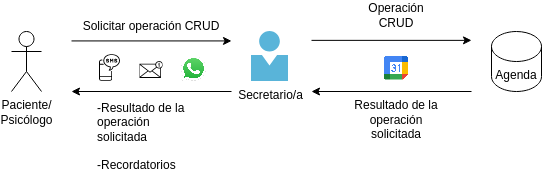
\includegraphics[scale=0.7]{doc/imagenes/flujo-tradicional.png}}
    \caption{Flujo tradicional adaptado a la Clínica Carmen Verdejo para la gestión de citas}
    \label{fig:flujo-tradicional}
\end{figure}

Observamos que un paciente o psicólogo para realizar cualquier gestión sobre sus citas siempre ha de pasar por un intermediario, quien se encarga de interactuar de forma directa con la agenda, en este caso Google Calendar. Es indiscutible que el hecho de que exista un intermediario ralentiza el proceso. Asimismo el canal de comunicación con el paciente puede conllevar a errores. \bigskip

A continuación se analizarán las herramientas utilizadas por la clínica para obtener una valoración de las mismas y determinar su utilidad en Carmen Verdejo.

\subsubsection*{Google Calendar}

\begin{figure}[H]
    \centering{
\includegraphics[scale=0.07]{doc/imagenes/google-calendar-logo.png}}
    \caption{Logo de Google Calendar}
    \label{fig:google-calendar}
\end{figure}

Google Calendar es un calendario online desarrollado por Google para uso personal o empresarial que permite la creación y compartición de eventos y reuniones o la planificación de tareas, así como notificar próximos eventos del calendario con tanta antelación como desee el usuario. \bigskip

Como ya se ha explicado, la clínica Carmen Verdejo utiliza Google Calendar a modo de agenda para gestionar las citas de los pacientes con el equipo de psicólogos. A este calendario sólo tiene acceso Carmen María quien es la única persona del equipo con el poder de crear, modificar, consultar o borrar citas, si alguno de los psicólogos desea realizar alguna de estas operaciones debe de solicitárselo a Carmen María. \bigskip

Tras conocer el uso de Google Calendar en la clínica, es momento de examinar la plataforma. En primer lugar hay que mencionar que un gran punto positivo es que es totalmente gratis, exceptuando su uso a través de SMS. Por supuesto también hay que destacar la experiencia de usuario ofrecida lo cual ya hizo Tanya Feddern-Beckan de la Escuela Miller de la Universidad de Miami en su artículo 'Google Calendar' \cite{FeddernBekcan2008}. Feddern resalta en lo referente a usabilidad, la alta personalización ofrecida: tamaño de fuente, idioma, formato de fecha y hora, zona horaria, colores... Adicionalmente la plataforma es totalmente responsiva adaptándose al tamaño de cualquier dispositivo y pudiendo funcionar en la mayoría de navegadores. Por otro lado, la personalización ya mencionada junto con el uso correcto de contrastes y grandes elementos visuales en los que hacer click la convierten en una aplicación bastante accesible para un gran abanico de tipos de usuario. \bigskip

Sin embargo, es tan profunda la personalización que puede llevarse a cabo en Google Calendar que un usuario con poca o media experiencia en el uso de este tipo de plataformas, desconoce las numerosas posibilidades que ofrece una herramienta tan potente. Un claro ejemplo de ello es el no uso de 'Calendarios Masters' en los que el usuario creador del calendario puede administrar los permisos que poseen los usuarios invitados al calendario. Esto permitiría que el resto del equipo no tuviera la necesidad de acudir a Carmen María para cualquier gestión sobre las citas. \bigskip

Queda claro con esta evaluación que Google Calendar es una muy buena herramienta para usar como agenda online para uso personal, pero no tanto para empresarial si los usuarios no están experimentados en el uso de este tipo de plataformas, por lo que en ese caso no es posible exprimir todo su potencial.

\subsubsection*{WhatsApp, correo electrónico y SMS}

WhatsApp, el correo electrónico y los SMS se tratan de servicios utilizados por la clínica Carmen Verdejo cuya combinación hace posible la comunicación a distancia con la mayoría de sus pacientes. Para los dos primeros se necesita acceso a Internet y ya se vio en el capítulo \ref{intro} que un 93.9\% de la población española entre 16 y 74 años usó Internet en el año 2021, de acuerdo a un estudio del INE. En cuanto a los SMS, un 99.5\% de la población en ese mismo estudio disponía de un teléfono móvil. Por lo cual el servicio de comunicación ofrecido por la clínica a sus pacientes es prácticamente accesible a todo el mundo. \bigskip

Sin embargo, a pesar de la extensión de su uso en España dichos medios de comunicación poseen desventajas, algunas de las cuales han sido destacadas por la clínica. Por ejemplo, el pago de los mensajes por SMS o la desconfianza generada por las alteraciones en la red que evoquen a un no correcto envío de los mensajes. Estas son algunas de las desventajas de las que un usuario medio es conocedor, no obstante un punto muy negativo que se ha de mencionar en este caso de estudio es el tratamiento de los datos por parte de WhatsApp y en el transporte de estos por parte de algunos proveedores de correo electrónico. \bigskip

Por una parte, WhatsApp es una aplicación de mensajería instantánea de la cual es propietaria actualmente Meta, una gran empresa estadounidense que ha sido causa de grandes polémicas en relación a la protección de datos. En lo que concierne a una clínica como Carmen Verdejo, que es un centro sanitario, el Servicio Nacional de Salud de Inglaterra no aconseja su uso en este tipo de centros \cite{Gould2016-ky}, ya que algo tan sensible como los datos de los pacientes han ser protegidos ante cualquier vulnerabilidad. \bigskip

Por otra parte, Carmen Verdejo utiliza Gmail y de acuerdo a la estadísticas de la Figura \ref{fig:cifrado-correo} obtenidas en los Informes de Transparencia de Google \footnote{\url{https://transparencyreport.google.com/safer-email/overview?hl=es}}, el envío constante de mensajes cifrados desde Gmail a otros proveedores no es constante tal y como se ve en la figura. Por tanto, si el paciente receptor de un mensaje utiliza otro proveedor distinto a Gmail, Gmail no se puede encargar del cifrado del correo en el envío.

\begin{figure}[H]
    \centering{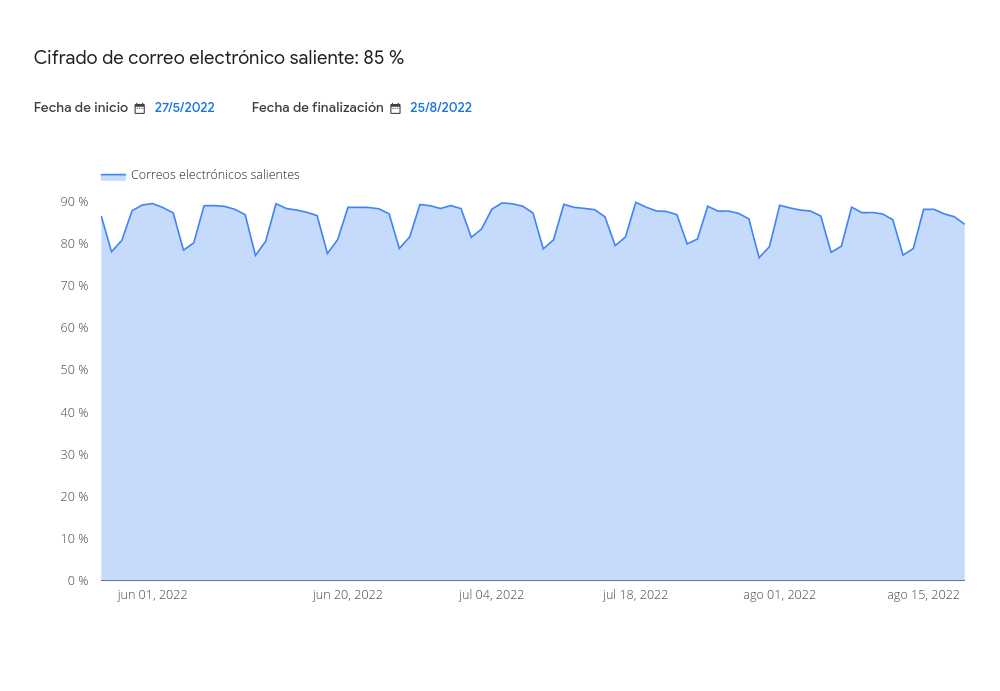
\includegraphics[scale=0.4]{doc/imagenes/cifrado-correo.png}}
    \caption{Cifrado de correo electrónico durante el envío de correo saliente en Google entre mayo y agosto de 2022}
    \label{fig:cifrado-correo}
\end{figure}

En definitiva, WhatsApp, el correo electrónico y los SMS son servicios muy completos, cómodos y útiles para la comunicación clínica-paciente, pero el peso de sus desventajas hace que se deba de considerar seriamente su sustitución por otros servicios de comunicación. 

\section{Soluciones para la gestión de citas online}
Después de haber conocido el día a día de la Clínica Carmen Verdejo en cuanto a la gestión de citas y las herramientas utilizadas para dicha labor, es momento de conocer otras opciones. Seguidamente, al igual que se ha hecho con las herramientas de Carmen Verdejo, se procede a realizar una evaluación de otros medios para la gestión de citas. Para ello se ha decidido analizar herramientas pensadas específicamente para la planificación de citas y herramientas genéricas de planificación cuyo fin no está especificado.

\subsection{Soluciones genéricas}

\subsubsection*{Notion}
\begin{figure}[H]
    \centering{
\includegraphics[scale=0.1]{doc/imagenes/notion-logo.png}}
    \caption{Logo de Notion}
    \label{fig:logo-notion}
\end{figure}

Notion \footnote{\url{https://www.notion.so}} es un software dirigido a la organización y planificación en cualquier marco de trabajo. A finales de 2021 acorde a la revista Forbes \footnote{\url{https://forbes.co/2021/10/11/emprendedores/notion-alcanza-una-valoracion-de-us10-000-millones-impulsada-por-el-trabajo-remoto-y-tiktok/}} ya contaba con más de 20 millones de usuarios, y es que esta plataforma conoce a la perfección qué necesita su público y cómo ofrecérselo. \bigskip

La plataforma hace uso de lo que ellos llaman \textit{Workspaces} \label{notion-workspaces} (espacios de trabajo) que son espacios colaborativos en los cuales un usuario o grupo de usuarios pueden gestionar su trabajo. Para lo cual se dispone de la creación de \textit{Páginas} que permiten al usuario crear una página en blanco o si se prefiere escoger entre una de las plantillas ofrecidas para crear una página como una lista de cosas por hacer, una agenda, un calendario, un tablero o incluso utilizarla como base de datos ya que permite la subida de archivos. Para mayor organización, se ofrece la posibilidad de almacenar páginas dentro de páginas, lo que equivaldría a disponer de carpetas. En adición a esto, con respecto a los espacios de trabajos Notion ofrece una jerarquía de usuarios diferenciando entre dos categorías:

\begin{itemize}
    \item \textbf{Usuarios internos al espacio de trabajo}: En este grupo de usuarios todos tienen acceso a todas las páginas del espacio de trabajo, así como editarlas y borrarlas, pero existe una subcategoría más que agrupa a los usuarios en dos grupos:
        \begin{itemize}
            \item \textbf{Administradores}: Aquellos que además de las funciones nombradas, pueden invitar o eliminar usuarios del espacio de trabajo, gestionar los pagos de éste y cambiar sus ajustes.
            \item \textbf{Miembros}: Sólo tienen permitido añadir, editar o eliminar páginas
        \end{itemize}
    
    \item \textbf{Usuarios externos al espacio de trabajo}: Notion denomina a este tipo de usuarios com o\textit{Guests} (huéspedes). Se tratan de usuarios que no pertencen al espacio de trabajo, pero que han sido invitados por un administrador a una o varias páginas. El administrador tiene la posibilidad de designar los privilegios de los que dispondrá el huesped sobre la página:.
        \begin{itemize}
            \item Compartir, editar y comentar
            \item Editar y comentar
            \item Comentar
            \item Sólo ver
        \end{itemize}
\end{itemize}

Adicionalmente cabe mencionar que cuenta con integraciones con Slack y Google Drive. \bigskip

Como se ha indicado es una herramienta destinada tanto para el uso individual como para el uso colaborativo de equipos y empresas. Sin embargo, la herramienta sólo es gratuita para uso individual con algunas limitaciones, si el usuario desea contar con más funcionalidades deberá de hacer la compra de uno de los planes que se muestran en la Figura \ref{fig:precios-notion}.

\begin{figure}[H]
    \centering{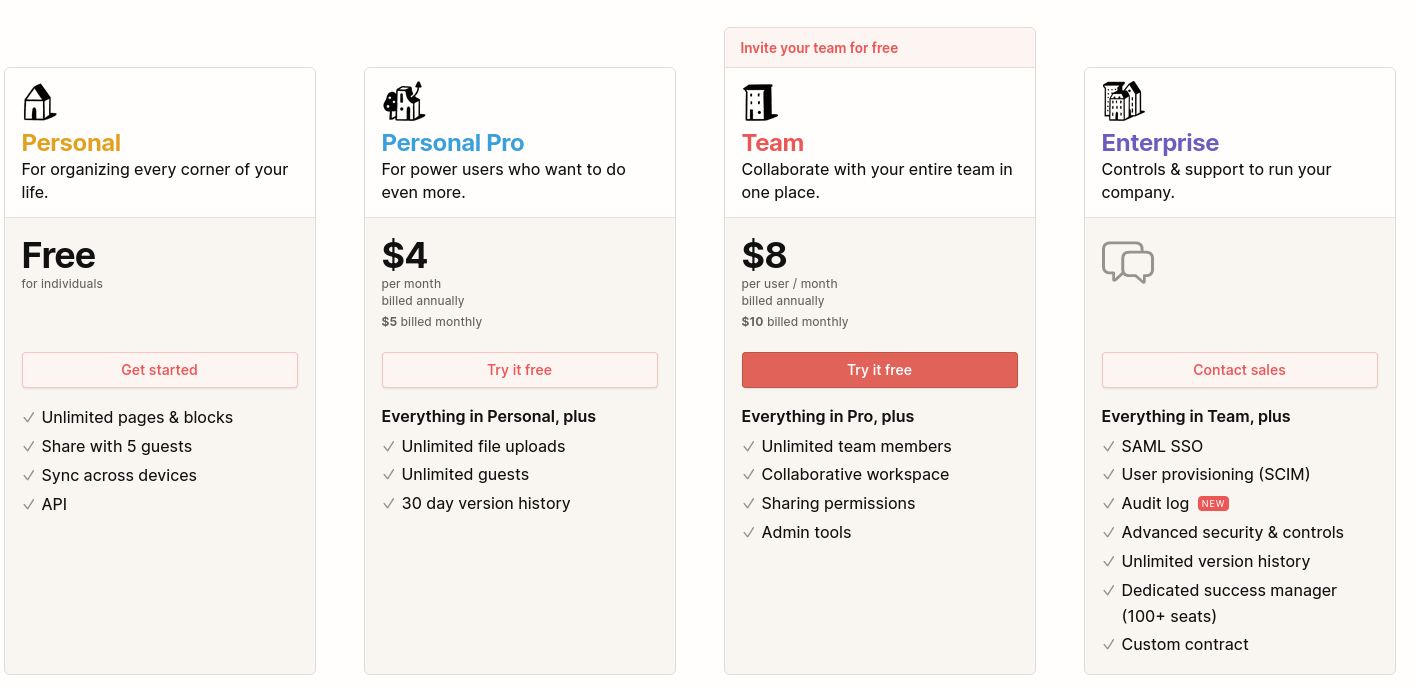
\includegraphics[scale=0.3]{doc/imagenes/precios-notion.png}}
    \caption{Planes de pago de Notion}
    \label{fig:precios-notion}
\end{figure}

En cuanto a lo que a Carmen Verdejo respecta con esta aplicación, la clínica podría hacer uso de la creación de páginas para que cada psicólogo dispusiera de una y dentro de dichas páginas se tuviera un calendario e información de las citas de todos sus pancientes. De esta forma agilizamos la comunicación psicólogo-secretaria de la Figura \ref{fig:flujo-tradicional}. Incluso a parte de la gestión de citas, la herramienta permitiría llevar un registro de pagos y documentación de los pacientes. Por otro lado, para la comunicación paciente-secretaria se tendría la posibilidad de añadir a los pacientes a su página correspondiente como huéspedes para gestionar sus citas, sólo se necesitaría que el paciente dispusiera de un correo electrónico para registrarse en Notion y conocimientos básicos en el uso de aplicaciones de este tipo. No obstante, aunque no dispusiera de esto último Notion tiene una guía \footnote{\url{https://www.notion.so/help/guides}} muy detallada sobre cómo usar la aplicación. \bigskip

Sin embargo, se ha indicado que para un trabajo colaborativo se debe de comprar uno de los dos planes de equipo, lo cual supone una importante cantidad de dinero al año teniendo en cuenta que el equipo está formado por x (PC) personas. Asimismo, otra desventaja de Notion es que sólo está disponible en inglés, francés, coreano y japonés, por lo que se da la posibilidad de que la plataforma no sea accesible para un determinado número de pacientes. \bigskip

En resumidas cuentas, Notion es una herramienta para la gestión de trabajo que ofrece infinitas posibilidades a sus usuarios para adaptar la herramienta a su ámbito de trabajo. Desde la clínica Carmen Verdejo ya se ha explicado cuál podría ser su papel en la gestión de citas, no obstante el alto precio a pagar y el idioma no compensa su uso. 

\subsubsection*{Asana}
\begin{figure}[H]
    \centering{
\includegraphics[scale=0.1]{doc/imagenes/asana-logo.png}}
    \caption{Logo de Asana}
    \label{fig:logo-asana}
\end{figure}

Asana \footnote{\url{https://app.asana.com}} es una plataforma desarrollada con objeto de ofrecer un servicio para gestionar el flujo de trabajo en equipos. A pesar de ello, es posible extender su uso a otros ámbitos como la gestión de citas online. \bigskip

La principal funcionalidad en el servicio brindado por Asana a sus usuarios es la creación de grupos de trabajos en los que los propios miembros del grupo pueden crear proyectos públicos para el resto del grupo o privados los cuales son sólo visibles a miembros del grupo invitados por el creador o por otros miembros que han sido invitados y tienen permisos de edición. Una vez que un proyecto ha sido creado, dentro del mismo los usuarios con permisos de edición pueden crear tareas organizadas por secciones cuya visibilidad puede ser controlada. En un proyecto los usuarios disponen de cuatro opciones para visualizar las tareas: en formato de calendario, como una lista, tablero o una línea temporal. Adicionalmente la plataforma ofrece reportes sobre el progreso de las tareas de un proyecto. \bigskip

Aparentemente Asana puede no parecer práctica para la planificación de citas, pero en realidad sí que se le puede sacar partido para ello, veamos a continuación cómo. La gestión de tareas con una fecha de entrega permite hacer una simulación en la que éstas se traten como citas y las secciones a las que pertenecen dichas ''tareas'' sean los pacientes en cuestión. Es decir, tendríamos tareas/citas asociadas a secciones/pacientes. Así mismo, se puede controlar la visibilidad de las citas para que cada psicólogo sólo tenga permisos de visualización y edición sobre las citas de sus pacientes y las pueda consultar a modo de agenda en el formato calendario de los proyectos. \bigskip

No obstante, Asana presenta algunos inconvenientes para su uso en la planificación de citas. Uno de estos inconvenientes es que a pesar del control de visibilidad que se puede aplicar sobre las tareas, las secciones no disponen de esta funcionalidad y los psicólogos tendrían visibles las secciones asociadas a pacientes que no son suyos. Añadido a esto, al comenzar a usar la herramienta su uso resulta muy poco intuitivo, en ningún momento se le explica al usuario los componentes de los que se forma la plataforma ni cómo usarlos. Por tanto, obligaría a éste a salir de la plataforma para buscar en su navegador tutoriales sobre su uso que son encontrados en la página oficial \footnote{\url{https://academy.asana.com/series/video-tutorials-tips}} , pero que desde dentro de la plataforma no son accesibles. \bigskip

Al igual que Notion, Asana dispone de tres planes a elegir para acceder a más y mejores funcionalidades. Entre ellas y la más importante para este análisis se encuentra la gestión de permisos. En la siguiente figura se muestran los precios junto con las funciones ofrecidas:

\begin{figure}[H]
    \centering{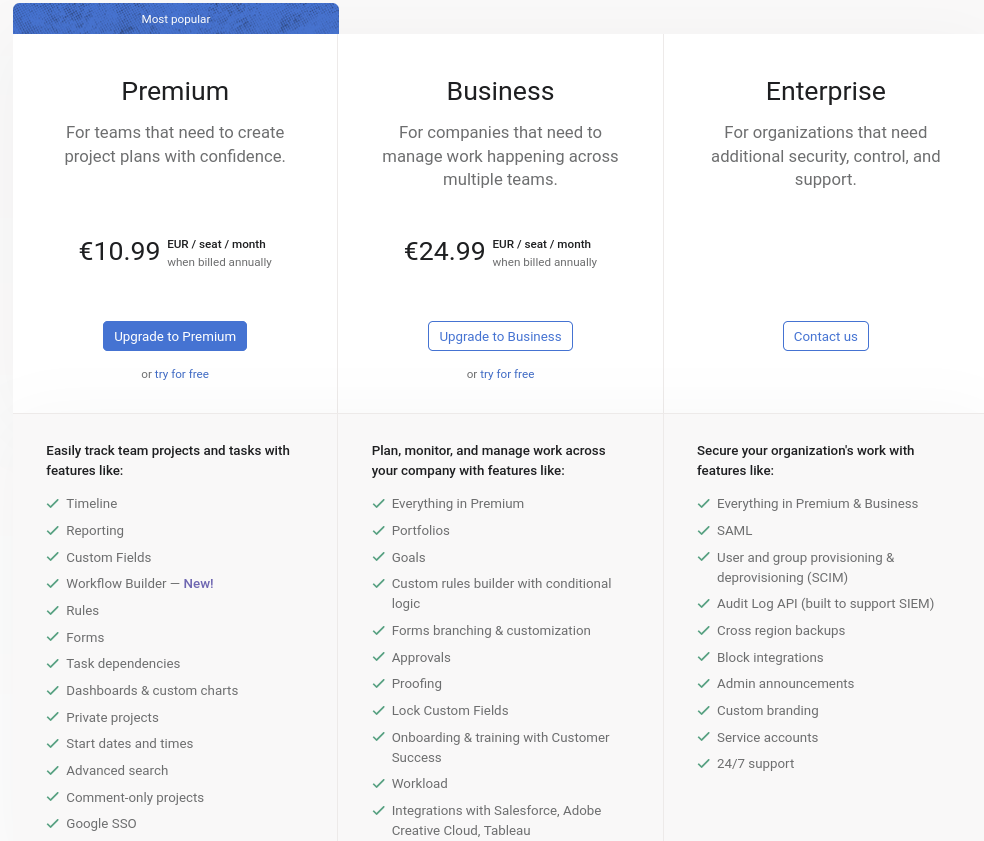
\includegraphics[scale=0.23]{doc/imagenes/asana-precios.png}}
    \caption{Planes de pago de Asana}
    \label{fig:asana-precios}
\end{figure}

Finalmente se ha de mencionar que la vía de comunicación psicólogo-secretario se vería mejorada, no obstante con Asana se hace muy difícil la adaptación para la comunicación paciente-secretario principalmente por la limitada gestión de permisos ofrecida en los packs. \bigskip

Con este análisis se concluye que Asana a pesar de ofrecer un servicio bastante aceptable para la gestión de citas resulta poco viable por su precio, limitaciones en la gestión de permisos y su imposibilidad para mejorar la comunicación paciente-secretario.


\subsubsection*{Trello}

\begin{figure}[H]
    \centering{
\includegraphics[scale=0.3]{doc/imagenes/trello-logo.png}}
    \caption{Logo de Trello}
    \label{fig:trello-logo}
\end{figure}

Trello \footnote{\url{https://trello.com}} es la plataforma por excelencia en la planificación digital de tareas para uso personal o corporativo.  A primera vista puede aparentar ser la herramienta que menos puede ofrecer en la gestión de citas entre todas las analizadas, pero está muy lejos de ello. Esta ''aparente sencillez'' resulta clave para que desde estudiantes hasta grandes multinacionales como Red Hat se decanten por utilizarla. \bigskip

La herramienta al igual que Notion presenta espacios de trabajo en los que el usuario dispone de la funcionalidad de creación y gestión de tableros. La visibilidad de los tableros puede ser restringida, para ello Trello distingue entre los siguientes tres niveles:

\begin{itemize}
    \item \textbf{Privado}: Sólo el creador y aquellos usuarios invitados pueden acceder y editar el tablero 
    \item \textbf{Espacio de trabajo}: El creador y los miembros del espacio de trabajo pueden acceder y editar el tablero
    \item \textbf{Público}: Todo el mundo tiene acceso al tablero, pero sólo los miembros del espacio de trabajo pueden editarlo.
\end{itemize}

Dentro de los tableros los usuarios crean \textbf{tarjetas} que son organizadas en \textbf{listas}. A cada tarjeta se le puede asignar un usuario con acceso al tablero, una fecha, archivos o etiquetas, además de poder personalizar su aspecto. No sólo eso, sino que también se puede decidir si recibir notificaciones cuando una tarjeta cambia su estado. También resulta relevante mencionar que Trello ofrece integraciones gratuitas con otras plataformas entre las que se encuentra Google Calendar. \bigskip

Por una lado, como se ha indicado Trello presenta integraciones entre las que se encuentra Google Calendar, lo cual resulta muy interesante para la clínica Carmen Verdejo que ya utiliza Google Calendar. Por otro lado, los psicólogos dispondrían de su propia ''agenda'' en forma de tablero con las citas de sus pacientes en forma de tarjetas gestionables tanto por la secretaria como por el psicólogo. Por tanto, la combinación del uso de Google Calendar y Trello abriría la posibilidad de que no sólo los psicólogos consultaran sus citas tanto por Trello como por Google Calendar, sino que también los propios pacientes pudieran hacerlo con la gestión de permisos ofrecida por Google Calendar y sus ''Calendarios Master''. \bigskip

Al igual que las otras dos soluciones, Trello cuenta los siguientes planes de pago en la Figura \ref{fig:trello-precios} para una mejora de las funcionalidades ofrecidas. 

\begin{figure}[H]
    \centering{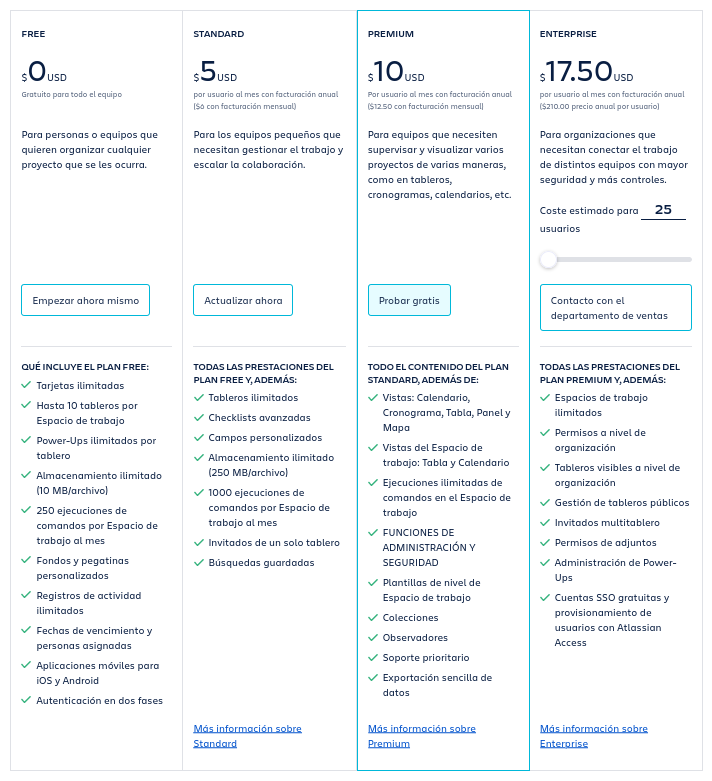
\includegraphics[scale=0.4]{doc/imagenes/precios-trello.png}}
    \caption{Planes de pago en Trello}
    \label{fig:trello-precios}
\end{figure}

Visualizando estos planes es evidente que para planificación de citas, el plan gratuito no es suficiente y en función del número de miembros del equipo de la clínica se tendría que optar por un plan de pago u otro. Seguidamente se explica por qué es conveniente en este caso decidirse por uno de los planes. \bigskip

Para empezar, por el limitado número de tableros ofrecidos en el plan gratuito, diez, ya que lo óptimo para su uso en la gestión de citas sería la creación de un tablero por psicólogo en el que cada tarjeta se asociara a una cita con un paciente. En adición a los planes de pago, si se quieren visualizar las tarjetas con otros formatos, como un calendario, se ha de contratar el plan Premium. Además, a pesar de las mejoras en la jerarquía de permisos, la jerarquía sólo se aplica a nivel de tablero, por lo que los pacientes no tendrían la posibilidad de hacer uso de Trello debido a que en dicha jerarquía aquel usuario invitado a un tablero independientemente de si puede editar o no, se le permite ver todas las tarjetas. Por tanto, un paciente vería las citas de otros pacientes y esto no se debe de permitir. Por tanto, para construir una agenda online con Trello mínimo se deberían de pagar aproximadamente diez euros mensuales por usuario. \bigskip

Definitivamente Trello resulta muy atractiva como solución con la integración gratuita de Google Calendar. No obstante, a pesar de su sencillo uso volveríamos a enfrentarnos con los mismos obstáculos presentados por Google Calendar para usuarios poco experimentados en el uso de estas plataformas y añadido a esto el gasto por un plan de pago para poder llevar a cabo la gestión de citas correctamente. Es por ello que su uso para este cometido no sería viable.


\subsection{Soluciones específicas}

\subsubsection*{ProDocfav}

\begin{figure}[H]
    \centering{
\includegraphics[scale=0.1]{doc/imagenes/logo-docfav.jpg}}
    \caption{Logo de ProDocfav}
    \label{fig:docfav-logo}
\end{figure}

ProDocfav \footnote{\url{https://pro.docfav.com/}} se ha elegido como la primera solución específica a analizar debido a que la clínica Carmen Verdejo se encuentra actualmente valorando su incorporación en su gestión de citas. \bigskip

Se trata de un software para clínicas perteneciente a la empresa vizcaína Docfav. Como la empresa indica en su página web oficial, tiene el propósito de gestionar el ciclo completo del paciente, es decir, no sólo las citas, sino también historial clínico, facturación e incluso la realización de consultas por videollamada. Por lo que Docfav promete ofrecer un servicio 360º en la gestión de pacientes. \bigskip

Para este análisis se va a utilizar su versión Demo gratuita que a pesar de tener una funcionalidad limitada, se puede recopilar más información acerca de su uso gracias a su manual de usuario \footnote{\url{ https://docfav.gitbook.io/docfav/}} que es público para todo el mundo . \bigskip

La plataforma tal y como se presenta resulta muy intuitiva a primera vista, pues en su vista principal el flujo seguido por sus usuarios (tanto profesionales, como pacientes) gira alrededor de la funcionalidad principal, la gestión de citas. Acompañada de una interfaz bastante agradable, el foco se pone en un calendario (Figura \ref{fig:docfav-calendario}) en el que se puede llevar a cabo la planificación de citas de los pacientes, pudiendo filtrar entre las agendas de los miembros de la clínica, los pacientes o los distintos servicios ofrecidos. Presenta un menú lateral que nos ofrece navegar a las secciones de gestión de clientes, facturación, estadísticas y ajustes, así como a la página externa correspondiente al manual del usuario. Cabe también mencionar que el software cuenta con integraciones con los calendarios de Google, Outlook, Apple... \bigskip

\begin{figure}[H]
    \centering{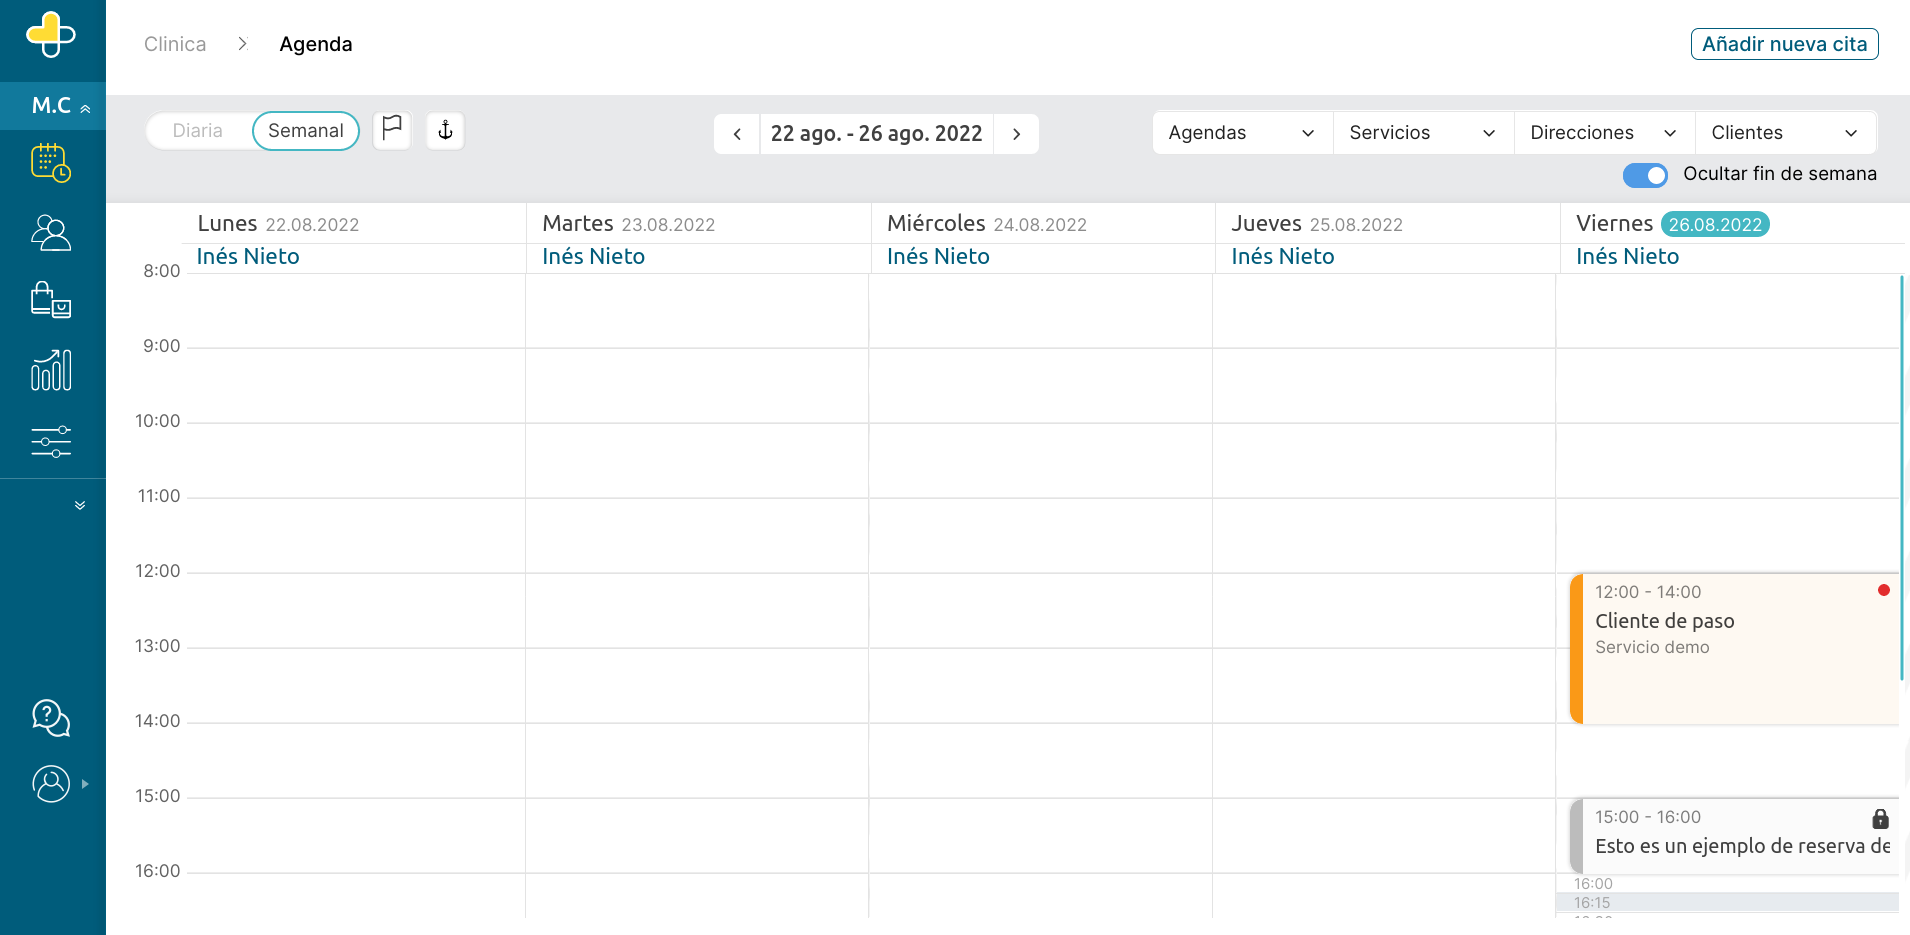
\includegraphics[scale=0.2]{doc/imagenes/docfav-calendario.png}}
    \caption{Sección principal de ProDocfav}
    \label{fig:docfav-calendario}
\end{figure}

Tras hacer una navegación por la plataforma y probar sus distintas funcionalidades, exceptuando la gestión del calendario, el resto de vistas se encuentran saturadas y no se aprecia ningún tipo de jerarquía visual, por ejemplo esto se puede comprobar en la vista de facturación, Figura \ref{fig:facturacion-docfav}:

\begin{figure}[H]
    \centering{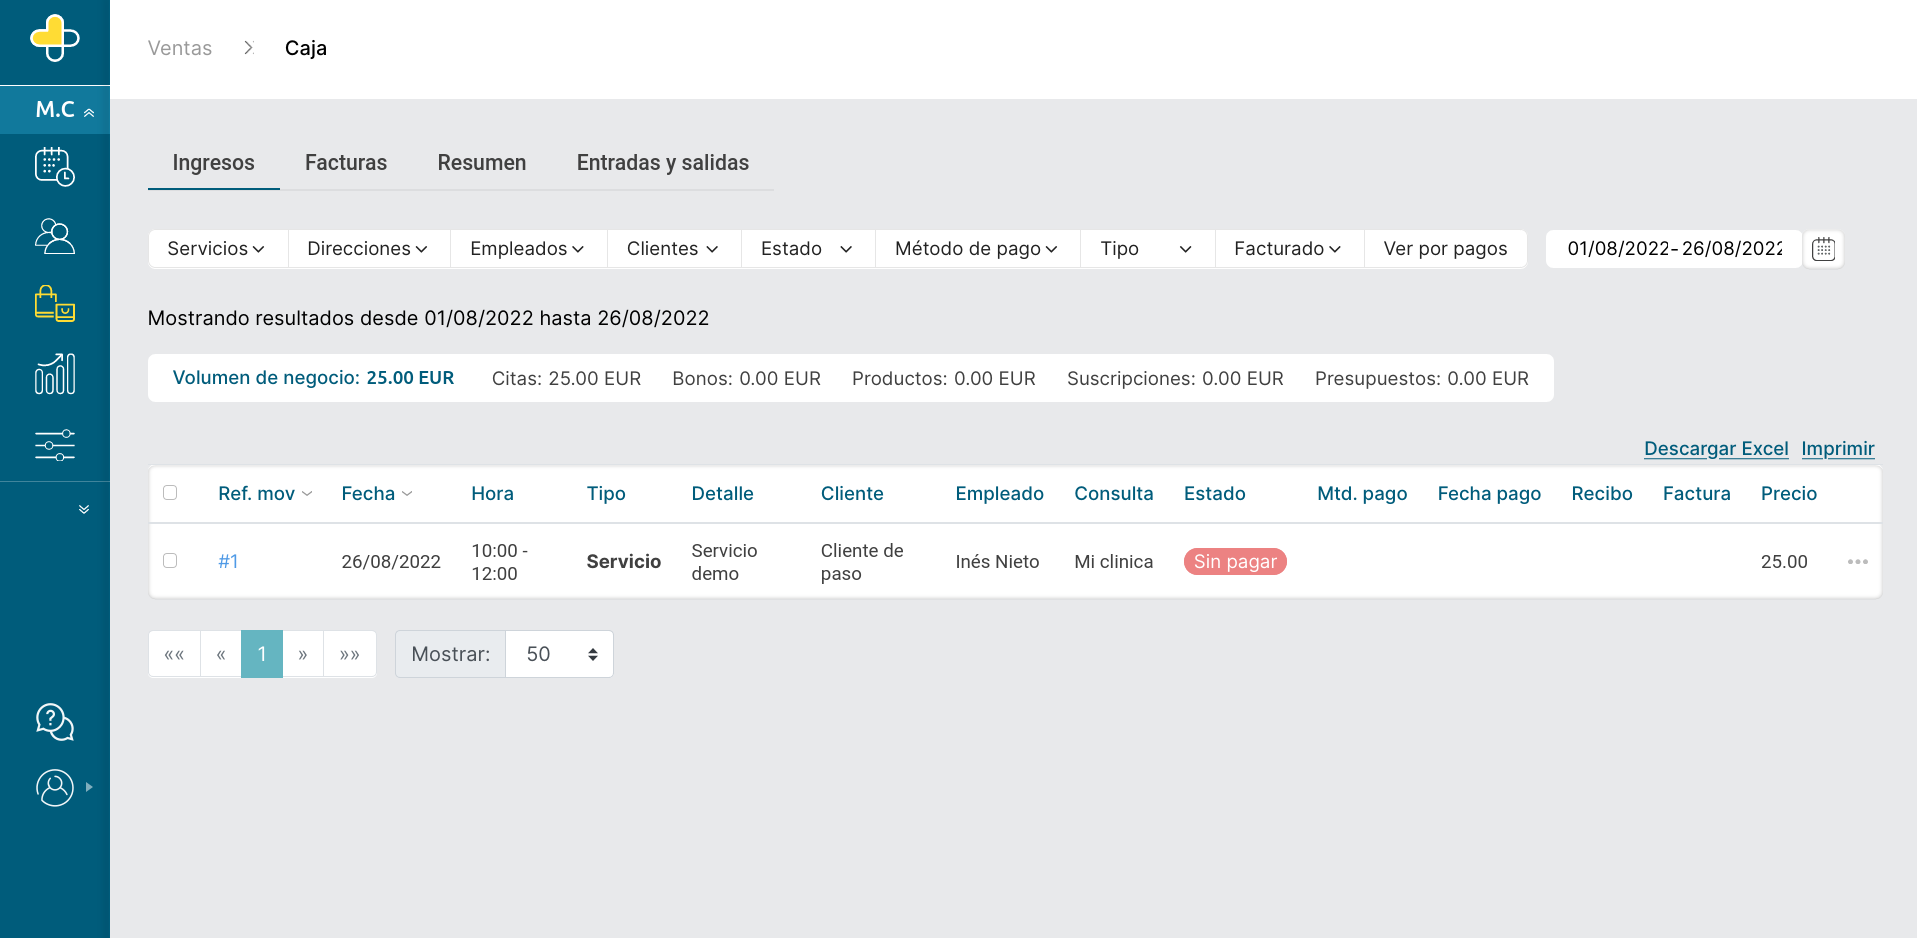
\includegraphics[scale=0.2]{doc/imagenes/facturacion-docfav.png}}
    \caption{Sección de facturación de ProDocfav}
    \label{fig:facturacion-docfav}
\end{figure}

De igual forma ocurre en la vista de los ajustes donde no se organizan las distintas acciones a realizar (Figura \ref{fig:ajustes-docfav}) y tan sólo se muestra un listado. Esto provoca a que el menú presentado resulte realmente incómodo de leer, pues de acuerdo a los principios de experiencia de usuario \cite{Scott2009-dh} para el ojo humano es mucho más fácil leer en vertical que en horizontal. Adicionalmente, debería de ser suficiente con leer el título de una opción del menú y no sobrecargar la vista con demasiado texto explicativo, como ocurre en este caso. 

\begin{figure}[H]
    \centering{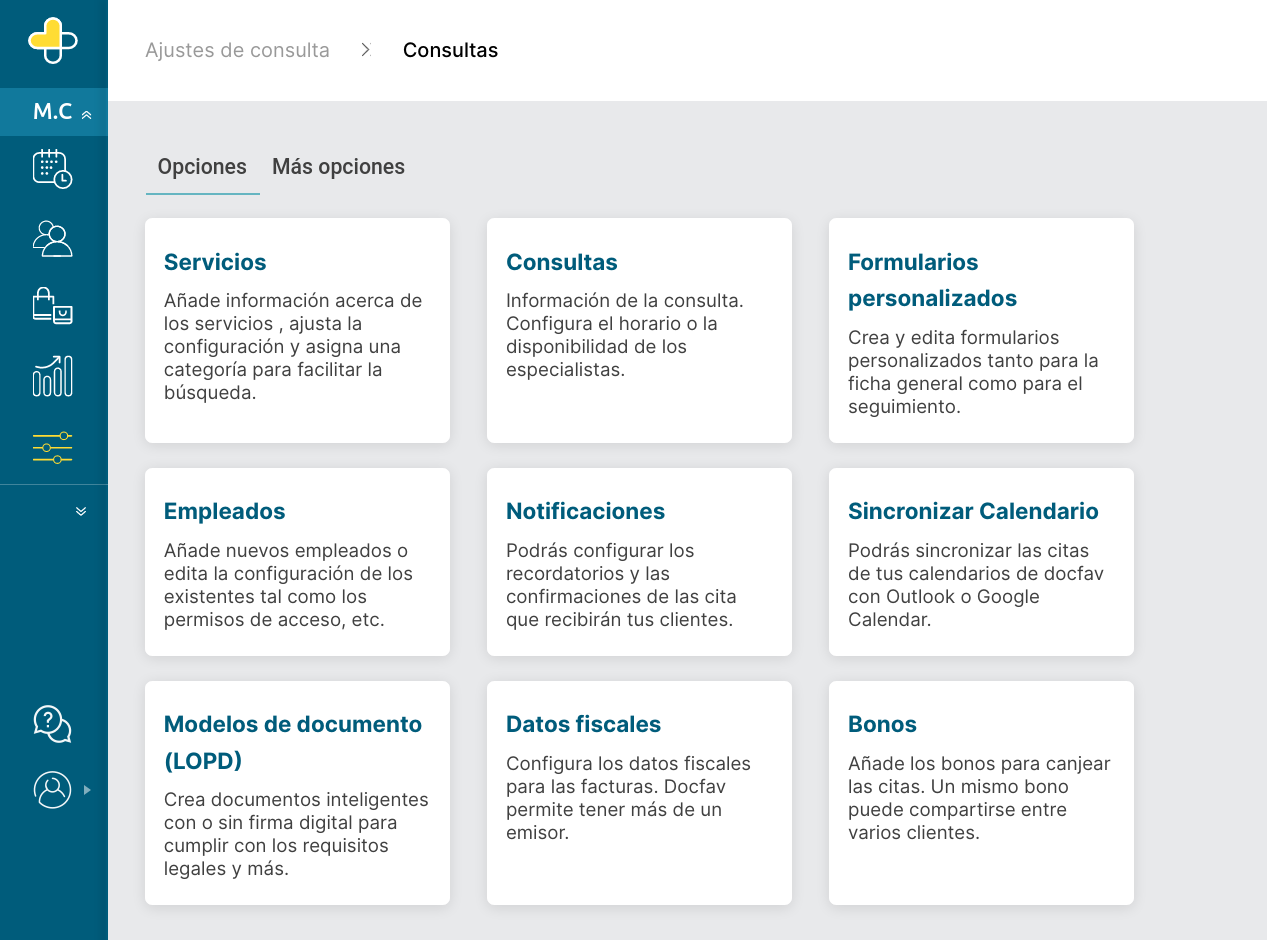
\includegraphics[scale=0.2]{doc/imagenes/docfav-ajustes.png}}
    \caption{Sección de ajustes de ProDocfav}
    \label{fig:ajustes-docfav}
\end{figure}

No obstante, estos defectos en el diseño de la interfaz que evocan a posibles confusiones en el uso de la plataforma se ven ligeramente compensados por la ayuda aportada por DocFav en su detallado manual del usuario. \bigskip

En cuanto al plan de precios, ProDocfav ofrece un sólo plan de pago de precio variante en función del número de trabajadores que utilicen el software. Por ejemplo, para diez trabajadores el precio a pagar de forma anual es de 62.42€ y de forma mensual de 74.90€. Desde luego un precio bastante alto en comparación a los planes de pago de las herramientas no específicas. \bigskip

En resumidas cuentas, ProDocfav a nivel de funcionalidad cubre con todas las necesidades que una clínica requiere para la gestión de sus citas y documentación. Sin embargo, parte de ese potencial se disipa si la experiencia de usuario acaba no siendo la mejor posible y más aún si no cumple con las expectativas de lo que se espera de un software de calidad de más de 60€ para diez usuarios. 

\subsubsection*{DriCloud}

\begin{figure}[H]
    \centering{
\includegraphics[scale=0.4]{doc/imagenes/dricloud-logo.png}}
    \caption{Logo de DriCloud}
    \label{fig:dricloud-logo}
\end{figure}

DriCloud \footnote{\url{https://dricloud.com/}} se define a sí mismo como  el mejor programa médico en la nube líder en 18 países. Sin duda alguna se trata de una contudente presentación que en pocas palabras suscita a cualquier usuario a tener grandes expectivas sobre este software. Es más, estas expectativas crecen aún más al conocer que instituciones de renombre como el Instituto Madrileño de Traumatología o el Instituto Andaluz de Neurología Pediátrica apuestan por su uso. \bigskip

Al igual que en el anterior caso, para el análisis de DriCloud se hará uso de la Demo proporcionada por la plataforma. No obstante, en este caso la demo está formada por una serie de vídeos explicativos sobre su uso. \bigskip

DriCloud ofrece gestión de citas de pacientes, de documentación (presupuestos, facturas, historiales clínicos...), guardado de firma digital, gestión de vacaciones de los trabajadores, creación de formularios de historia clínica,etc. Es decir, no sólo ofrece funcionalidades para la gestión de los pacientes, sino también funcionalidades para la gestión interna de la clínica. \bigskip

Dentro de la plataforma se distinguen una serie de roles para controlar las vistas a las que tiene permitido acceder un usuario. De acuerdo al video explicativo estos roles son los siguientes:

\begin{itemize}
    \item \textbf{Administrador del software}
    \item \textbf{Director}
    \item \textbf{Profesional}
    \item \textbf{Técnico} 
    \item \textbf{Secretaria}
    \item \textbf{Enfermera}
    \item \textbf{Contable}
\end{itemize}

Es importante mencionar que no existe una jerarquía explícitamente en la plataforma. Cada rol tiene asignadas unas vistas a las que puede acceder totalmente diferentes a las que tienen el resto de roles, por lo que si por ejemplo se desea crear un superusuario el usuario debe de tener todos los roles asignados. \bigskip

Centrándonos en el propósito que concierne a este proyecto, la gestión de citas online, DriCloud ofrece a los profesionales una \textit{Agenda}: 

\begin{figure}[H]
    \centering{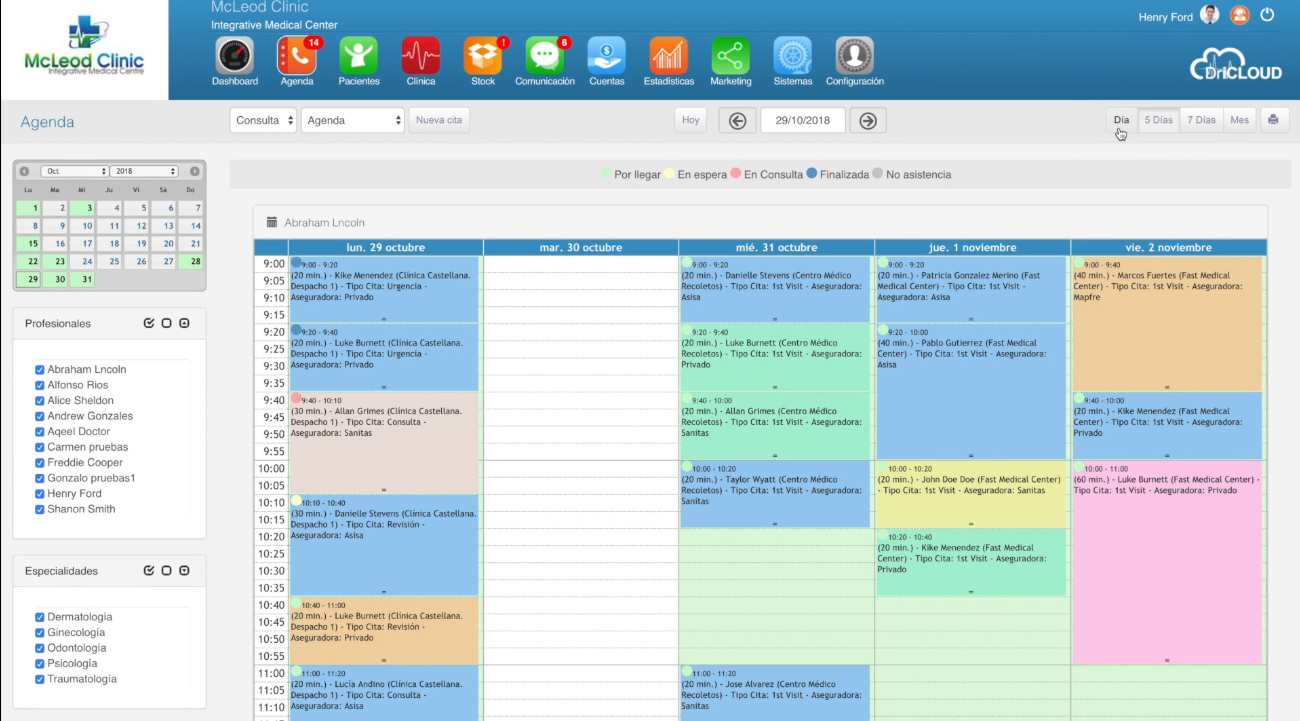
\includegraphics[scale=0.3]{doc/imagenes/dricloud-principal.png}}
    \caption{Vista principal de DriCloud para trabajadores}
    \label{fig:dricloud-principal}
\end{figure}

En esta agenda son destacables las siguientes características:

\begin{itemize}
    \item Las citas tienen asociado un estado (''Por llegar'',''En consulta'',''Finalizada'' y ''No asistencia'').
    \item Se da la opción de visualizar citas del día actual, los próximos cinco días, los próximos siete días o del resto del mes.
    \item Las citas pueden ser filtradas por profesional y/o especialidad.
    \item Dispone de tres modos de visualización:
    \begin{itemize}
        \item El modo \textbf{''Consulta''} que es el de la Figura \ref{fig:dricloud-principal}.
        \item El modo \textbf{''Planning''} en el que las citas se disponen como una línea temporal.
        \item El modo \textbf{''Dietario''} en el cual la información de las citas es mostrada en una tabla.
    \end{itemize}
\end{itemize}

En cuanto a los pacientes, DriCloud ofrece a sus clientes un código HTML para insertar en sus páginas un botón que permita realizar citas online. Este botón abre un formulario implementado por su equipo de desarrollo que el paciente deberá de rellenar para pedir una cita. Una vez el formulario haya sido enviado se le notifica la información de la cita al paciente vía SMS e email y dicha cita se crea en la agenda asociada al profesional que le atenderá. \bigskip

El servicio ofrecido a nivel funcional por DriCloud resulta realmente profundo, no sólo se puede hacer una gestión de citas y documentación de los pacientes, sino también del personal hasta el punto de hacer gestiones de recursos humanos como son la planificación de vacaciones. \bigskip

En lo que refiere a cuánto hay que pagar para acceder a estos servicios, se tienen varios planes de pago (Figura \ref{fig:dricloud-precios}). Si tomamos de referencia el plan de pago de ProDocfav, los precios son justificables ya que la plataforma ofrece más servicios. \bigskip

\begin{figure}[H]
    \centering{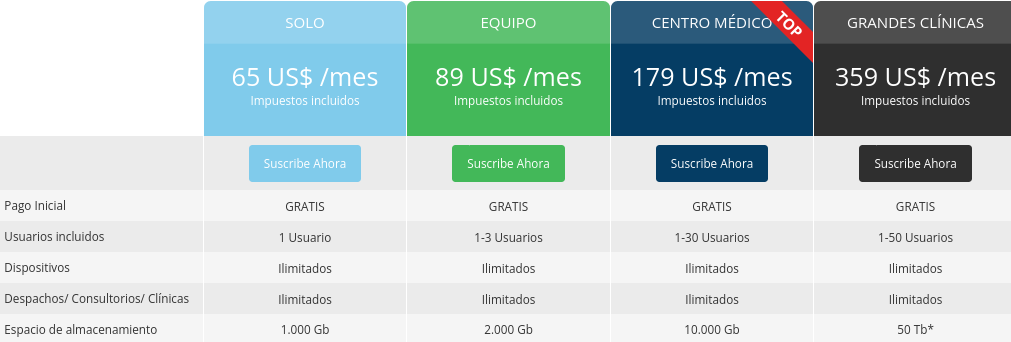
\includegraphics[scale=0.3]{doc/imagenes/dricloud-precios.png}}
    \caption{Planes de pago de DriCloud}
    \label{fig:dricloud-precios}
\end{figure}

Es claro que como usuario primerizo en la plataforma sin la ayuda ofrecida en los videos explicativos, resulta muy complicado entender su funcionamiento debido a las tantas funcionalidades proporcionadas. Se ha hecho durante los análisis anteriores bastante hincapié en el diseño de las interfaces, su usabilidad y accesibilidad ya que por muy buena y completa sea la funcionalidad ofrecida por una plataforma de nada sirve si no se le proporciona de forma correcta al usuario dicha funcionalidad. En esta herramienta encontramos al igual que en ProDocfav una importante saturación de la vista con texto innecesario (como el del menú de iconos o la leyenda de colores), iconos grandes y complejos, la no existencia de una jerarquía visual y el no uso de una paleta de colores. También hay que mencionar el uso del femenino en los roles \textit{Secretaria} y \textit{Enfermera} lo cual denota cierto sexismo. Se trata por tanto de una interfaz muy mejorable. \bigskip

El servicio de 24 horas proporcionado a los pacientes para solicitar una cita y el posterior envío de un SMS e email es un punto muy positivo, pero es incompleto ya que para modificar una cita, o incluso su consulta si se eliminase ese SMS o email, el paciente se debería de poner en contacto con la clínica.\bigskip

Para concluir, es evidente que una clínica como Carmen Verdejo conformada por PC x profesionales no le sacaría partido a esta herramienta. El plan de pago por el que se tendría que optar sería el de 179 euros mensuales para puedan acceder entre 1-30 usuarios y esto obliga a contratar un espacio de almacenamiento de 10 000Gb. Se trata pagar por un servicio que cubre mucho más allá de las necesidades de la clínica para finalmente seguramente no utilizar ni casi la mitad de todo lo ofrecido en dicho servicio. Para empresas y clínicas más grandes con varios establecimientos sí valdría la pena, pero en el caso de estudio de este proyecto definitivamente no.

\subsubsection*{Archivex}

\begin{figure}[H]
    \centering{
\includegraphics[scale=0.7]{doc/imagenes/archivex-logo.jpg
    }}
    \caption{Logo de Archivex}
    \label{fig:archivex-logo}
\end{figure}

 Archivex \footnote{\url{https://archivexclinical.com/}} es un software de gestión de clínicas desarrollado por Xoborg Technologies S.L en Salamanca. En su página oficial prometen que con el uso de Archivex la gestión de las clínicas de sus clientes se convertirá en un proceso sencillo en el que se ahorrará tiempo y dinero. Para evaluar la veracidad de estas palabras se hará uso de la demo ofrecida de siete días, así como de los vídeos explicativos disponibles en su canal de Youtube \footnote{\url{https://www.youtube.com/channel/UCGYoa8th_3iIZk1Zk9OGJTA}}. \bigskip

Archivex puede utilizarse en ordenadores con sistema operativo Windows o macOs, tablets y móviles Android o iOS. La plataforma al igual que el resto de soluciones anteriores, pone el foco de su vista principal en la agenda de sus profesionales, pero con algunas diferencias. En su vista principal llamada ''Hoy'' (Figura \ref{fig:archivex-principal} ) se presenta al usuario el personal de la clínica junto con la hora y paciente de su próxima cita si la hubiera. Si se hace click sobre uno de los profesionales, el usuario navegaría a la agenda semanal del profesional seleccionado (Figura \ref{fig:archivex-agenda-profesional} ). 

\begin{figure}[H]
    \centering{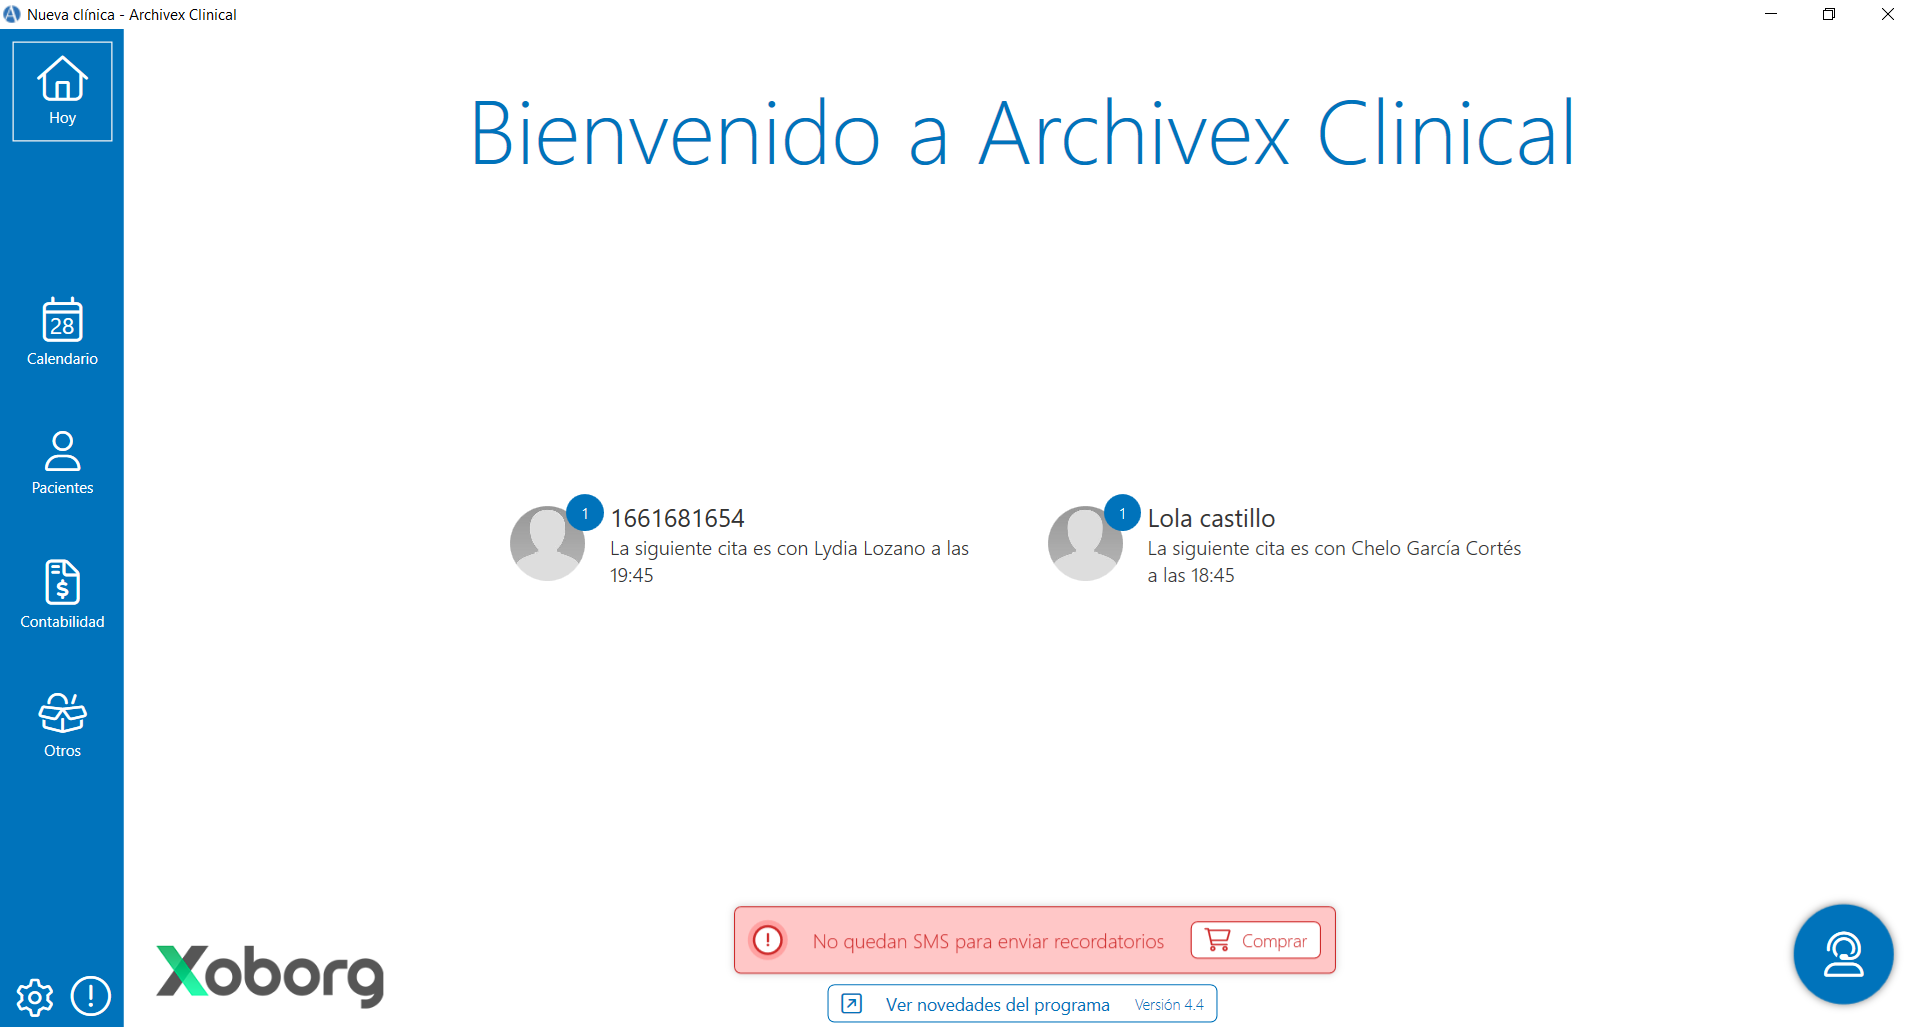
\includegraphics[scale=0.3]{doc/imagenes/archivex-principal.png
    }}
    \caption{Vista principal de Archivex}
    \label{fig:archivex-principal}
\end{figure}

\begin{figure}[H]
    \centering{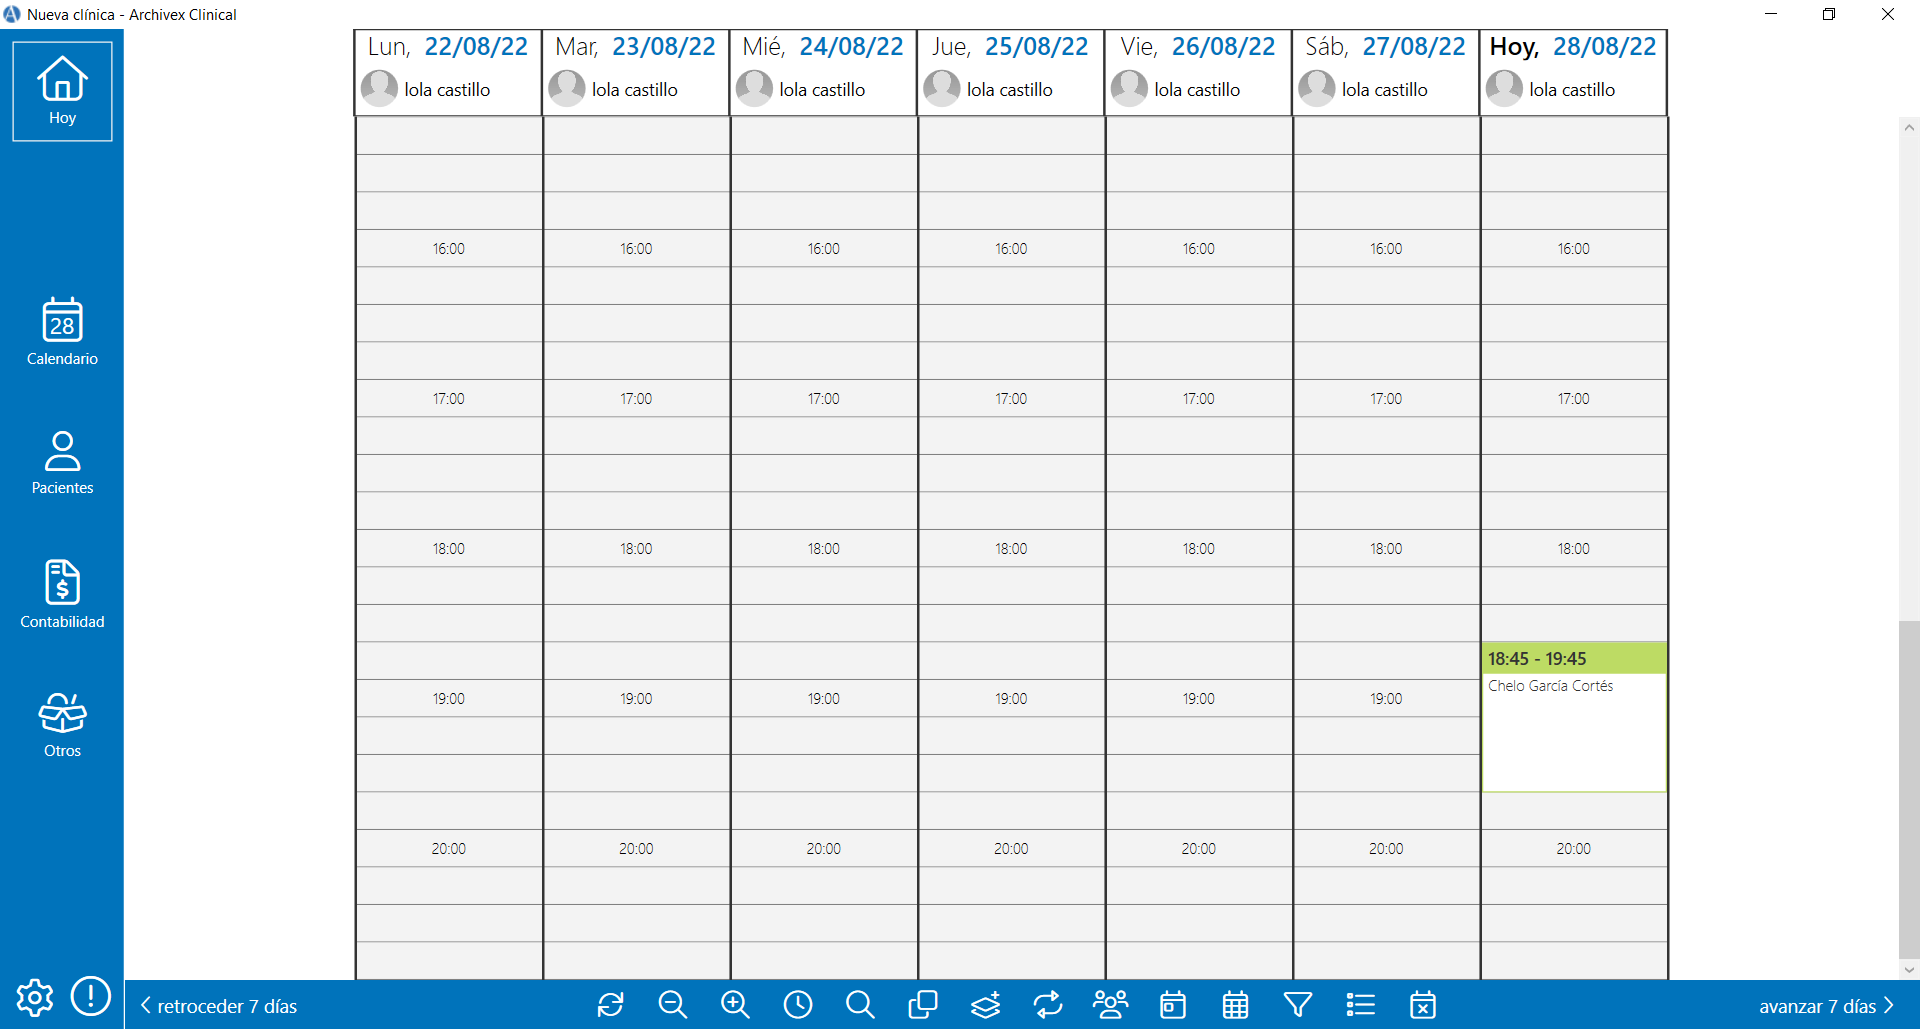
\includegraphics[scale=0.3]{doc/imagenes/archivex-agenda-profesional.png
    }}
    \caption{Vista semanal de la agenda de un profesional Archivex}
    \label{fig:archivex-agenda-profesional}
\end{figure}

En cuanto a la vista del ''Calendario'' (Figura \ref{fig:archivex-calendario}), nuevamente el usuario se toparía con la elección de escoger a uno de los profesionales para navegar a la vista de la Figura \ref{fig:archivex-agenda-profesional}. Además, tiene también la posibilidad de visualizar las citas por día de todos los profesionales (Figura \ref{fig:archivex-agenda-todos}  )

\begin{figure}[H]
    \centering{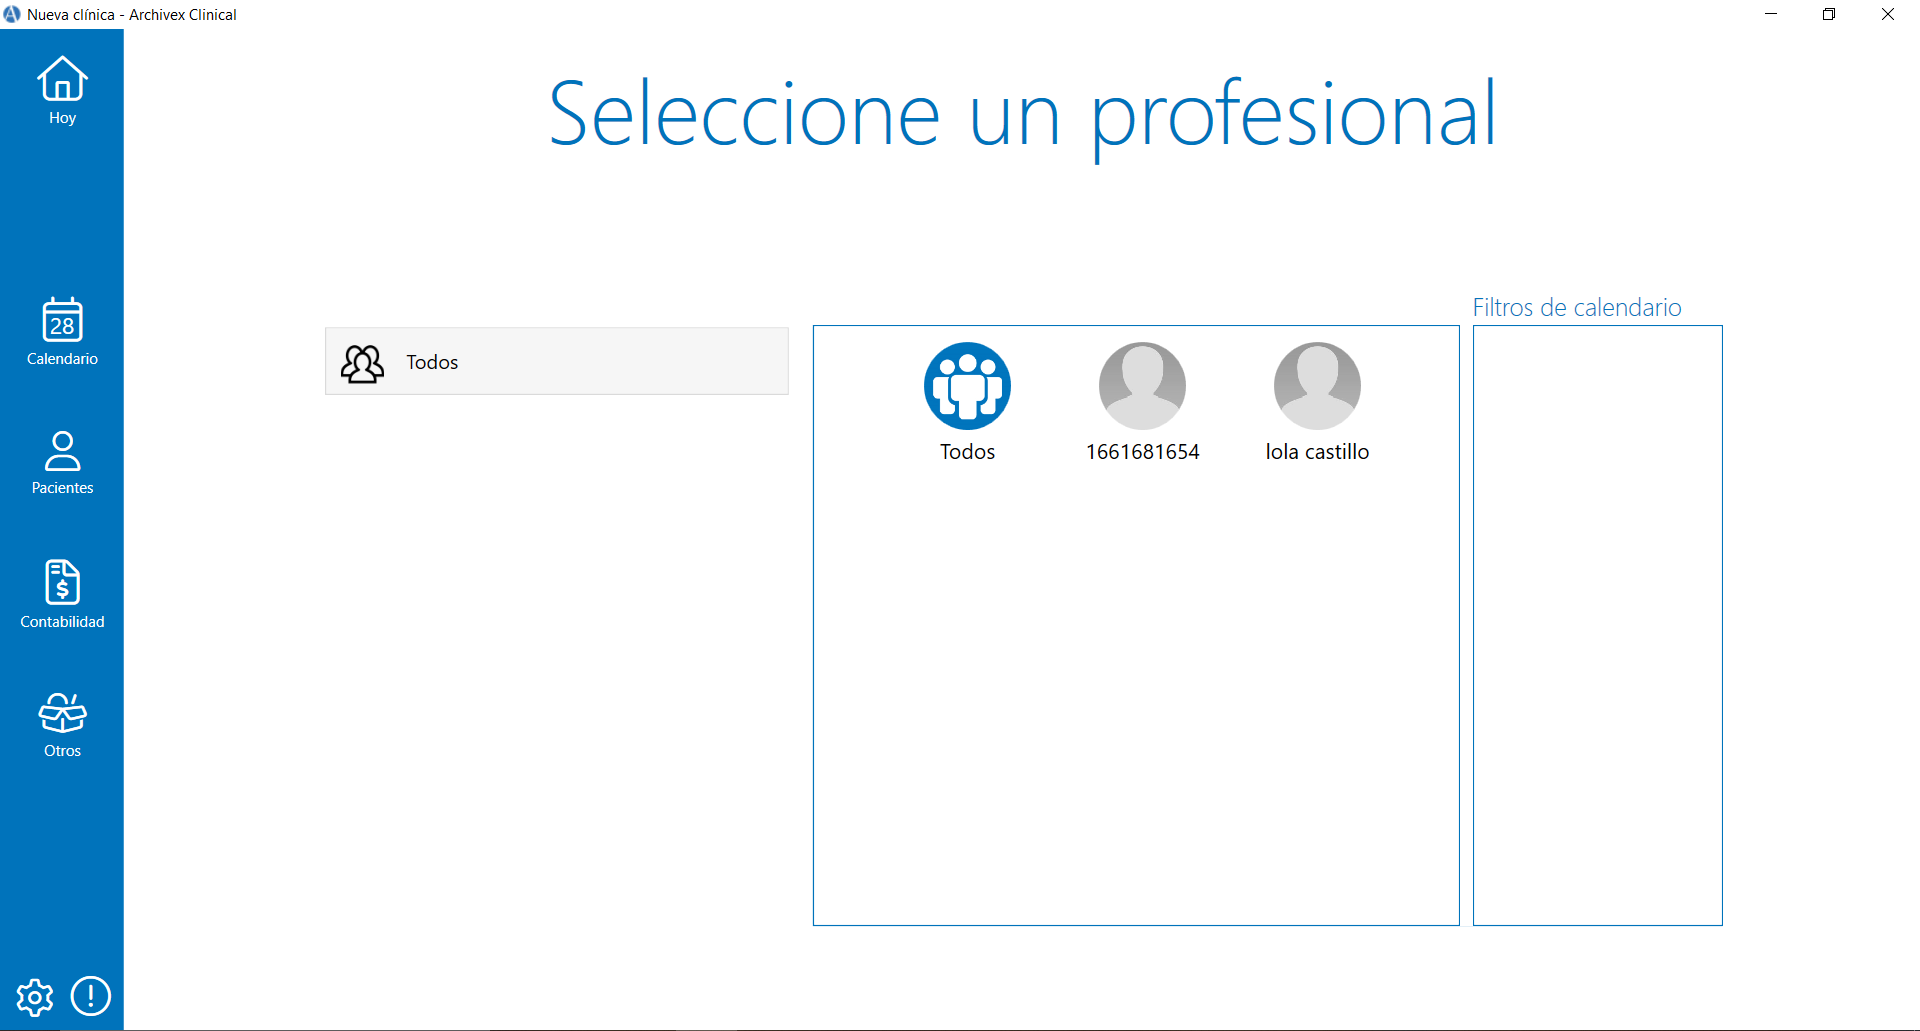
\includegraphics[scale=0.3]{doc/imagenes/archivex-calendario.png
    }}
    \caption{Vista de la sección ''Calendario''}
    \label{fig:archivex-calendario}
\end{figure}

\begin{figure}[H]
    \centering{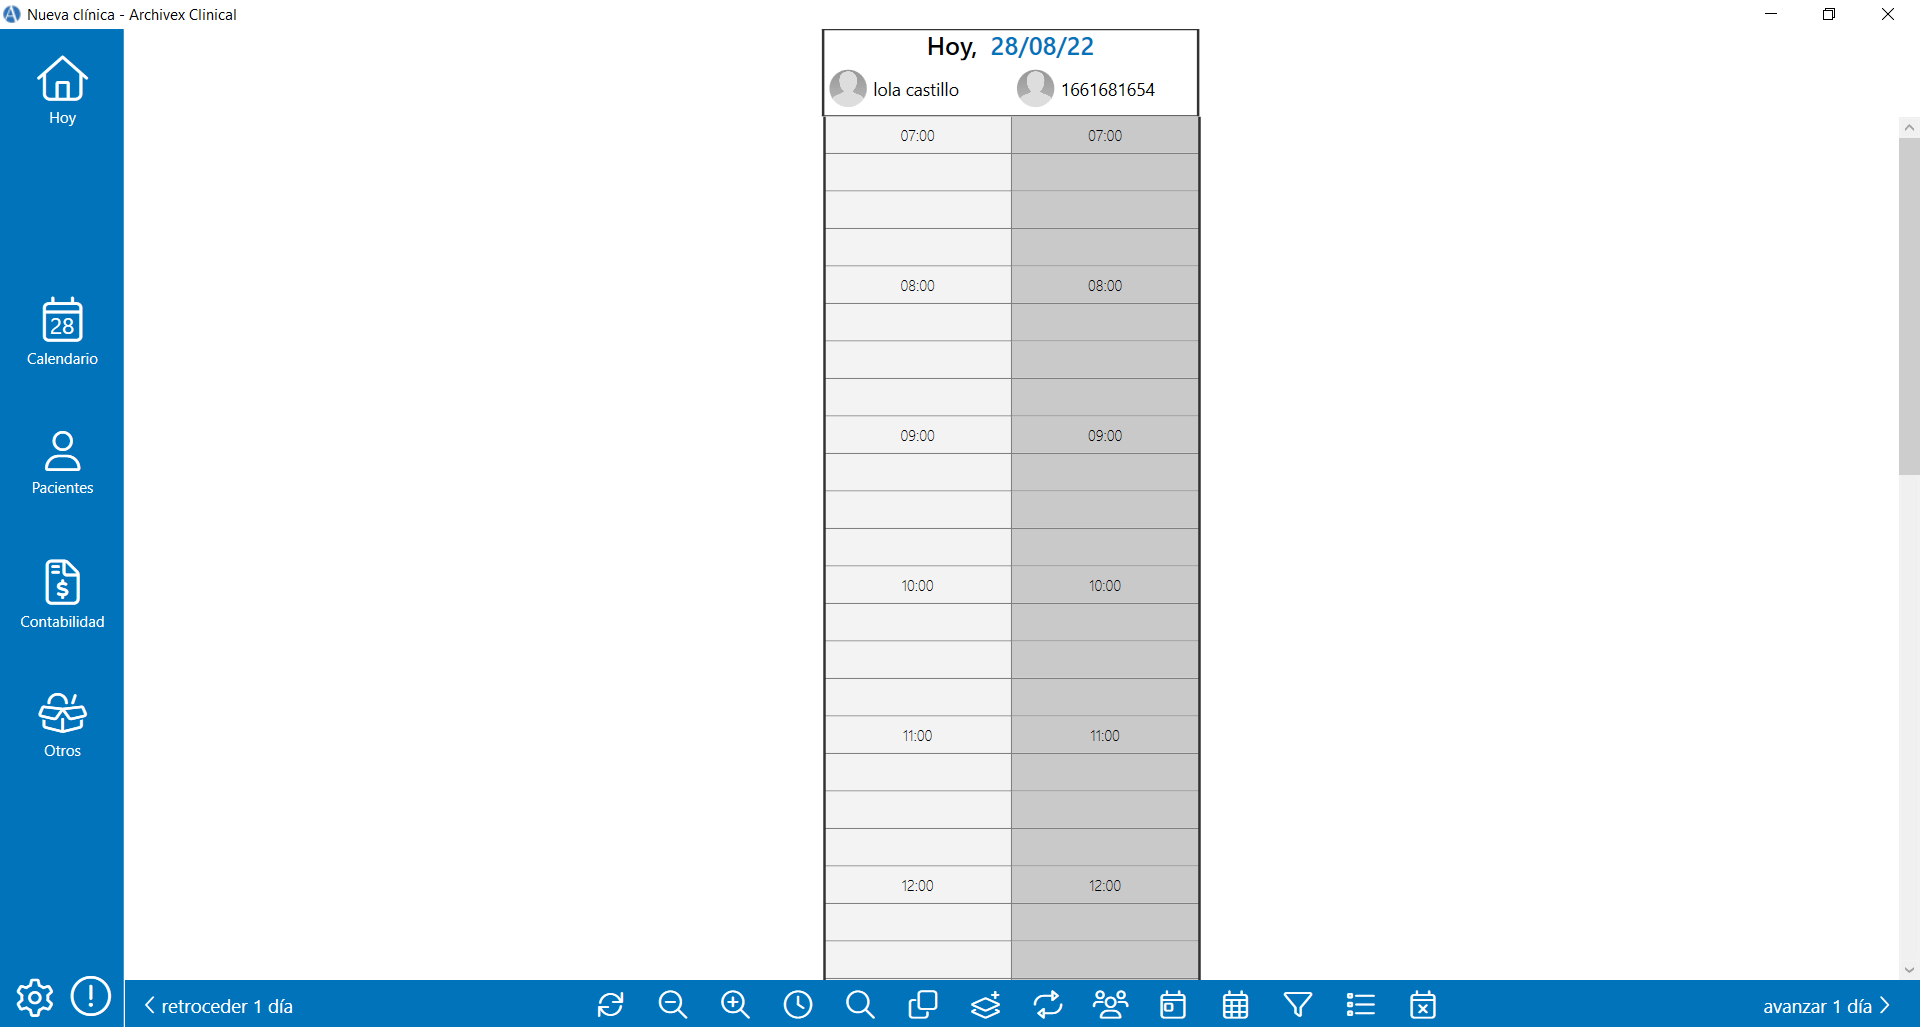
\includegraphics[scale=0.3]{doc/imagenes/archivex-agenda-todos.png
    }}
    \caption{Agenda del día actual de todos los profesionales}
    \label{fig:archivex-agenda-todos}
\end{figure}

En esta vistas en las que se muestra un calendario el usuario puede filtrar las citas por días de la semana y profesionales o avanzar o retroceder siete días (o un día si se trata de la vista de las citas de todos los profesionales). En adición a la gestión de citas, estas pueden ser notificadas a los pacientes vía WhatsApp redirigiendo al usuario al chat de WhatsApp Web asociado al número guardado en la ficha del cliente o vía SMS si se ha pagado por uno de los paquetes de pago de la Figura \ref{fig:archivex-sms} cuyo precio varía en función del número de SMS a pagar. \bigskip

\begin{figure}[H]
    \centering{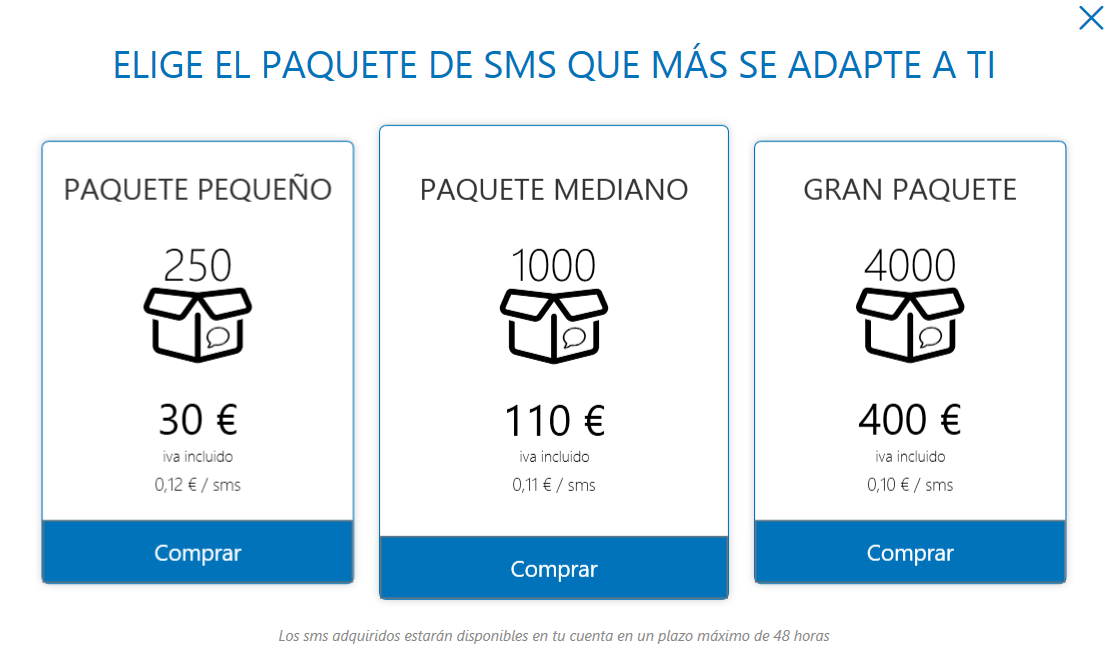
\includegraphics[scale=0.3]{doc/imagenes/archivex-sms.png
    }}
    \caption{Planes de pago de SMS}
    \label{fig:archivex-sms}
\end{figure}

Los clientes disponen con Archivex de un servicio 24 horas para gestionar sus citas. Para ello, tan sólo han de acceder a la página web de la clínica y pulsar sobre el botón de pedir cita que habrá de haber incorporado la propia clínica a su página con anterioridad. El paciente será redirigido a un inicio de sesión en el que deberá de introducir su DNI, una vez realizado esto recibirá un código por SMS o por correo electrónico que le permitirá acceder a la gestión de sus citas. En caso de que fuera su primera vez utilizando la plataforma el usuario se podrá registrar rellenando un formulario. \bigskip

A parte de la gestión de citas, Archivex también ofrece hacer una gestión del historial clínico de los pacientes, así como manejar la facturación de la clínica entre otros servicios secundarios (controlar stock, acceder a estadísticas, gestión de la información de aseguradoras, etc.). El acceso a estos servicios de acuerdo a los videos explicativos está restringido en función del rol del usuario, no obstante no se aporta más información acerca de los roles. \bigskip

En cuanto a precio, en la Figura \ref{fig:archivex-precio} se muestran los planes de pago:

\begin{figure}[H]
    \centering{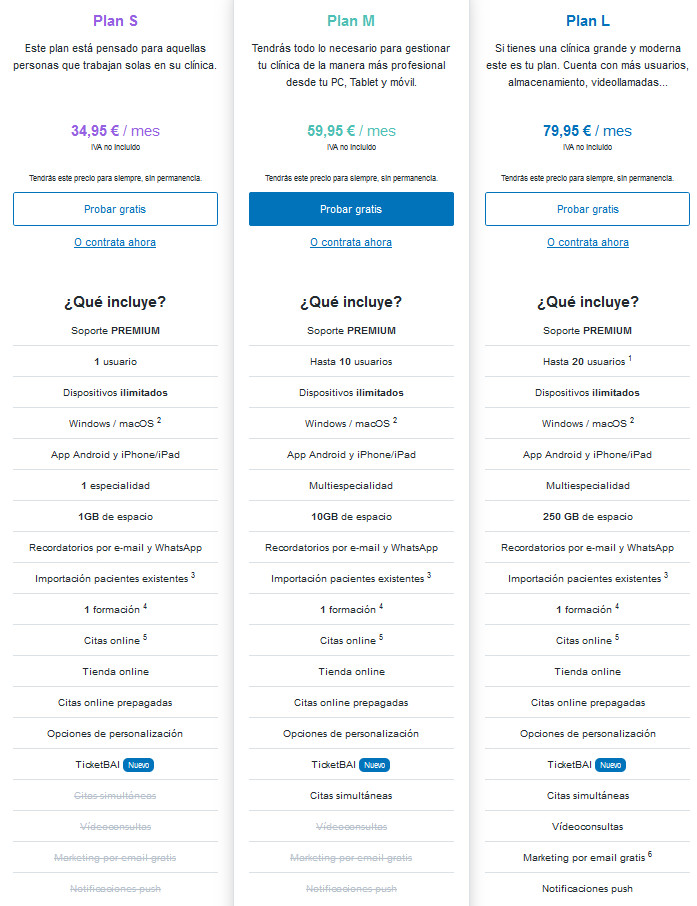
\includegraphics[scale=0.3]{doc/imagenes/archivex-precios.png
    }}
    \caption{Planes de pago de Archivex}
    \label{fig:archivex-precio}
\end{figure}

Tras conocer el servicio ofrecido por Archivex y haber probado su demo, la presentación sobre ahorro de tiempo y dinero aportada por la empresa de la herramienta no es del todo veraz. Veamos a continuación por qué:

\begin{itemize}
    \item \textbf{El tiempo}: Un usuario primerizo en el uso de la herramienta, aún visualizando los vídeos explicativos o leyendo su documentación tendría que gastar bastante de su tiempo aprendiendo a usar la herramienta. Esto se debe a que no se ofrece un tour al iniciar por primera vez sesión en la plataforma, los vídeos explicativos se centran mayormente en la gestión de citas, dejando sin cubrir otras funcionalidades como la gestión de la documentación. A esto se le suma la redundancia que aportan las vistas ''Hoy'' y ''Calendario'', una sóla vista del calendario y funciones de filtrado de citas sería suficiente. De nuevo no existe jerarquía visual, al usuario no se le indica en qué vista se encuentra y los formularios son como el de la Figura \ref{fig:archivex-crear-citas} donde se debe de hacer un recorrido visual en zigzag que aumenta la dificultad para leerlo. Además son tantos los servicios secundarios ofrecidos y la escasa documentación asociada a ellos que el usuario tendría que invertir tiempo en aprender sobre su uso. 
    \item \textbf{El dinero}: Los planes de pago se diferencian sobretodo en el espacio de almacenamiento y el número de usuarios. Aprovechar o no un plan de pago dependería en función del volumen de documentación generada por cada usuario, lo cual estaría vinculado al número de pacientes. Si se tratara de una clínica grande con un gran número de pacientes y en consecuencia con un gran número de personal el Plan L que es el que mayores ventajas aporta al usuario posiblemente no sea suficiente. En cambio en el otro extremo, Plan S, 1Gb de espacio de almacenamiento aún sólo tratándose de un usuario tampoco sería suficiente.
\end{itemize}

\begin{figure}[H]
    \centering{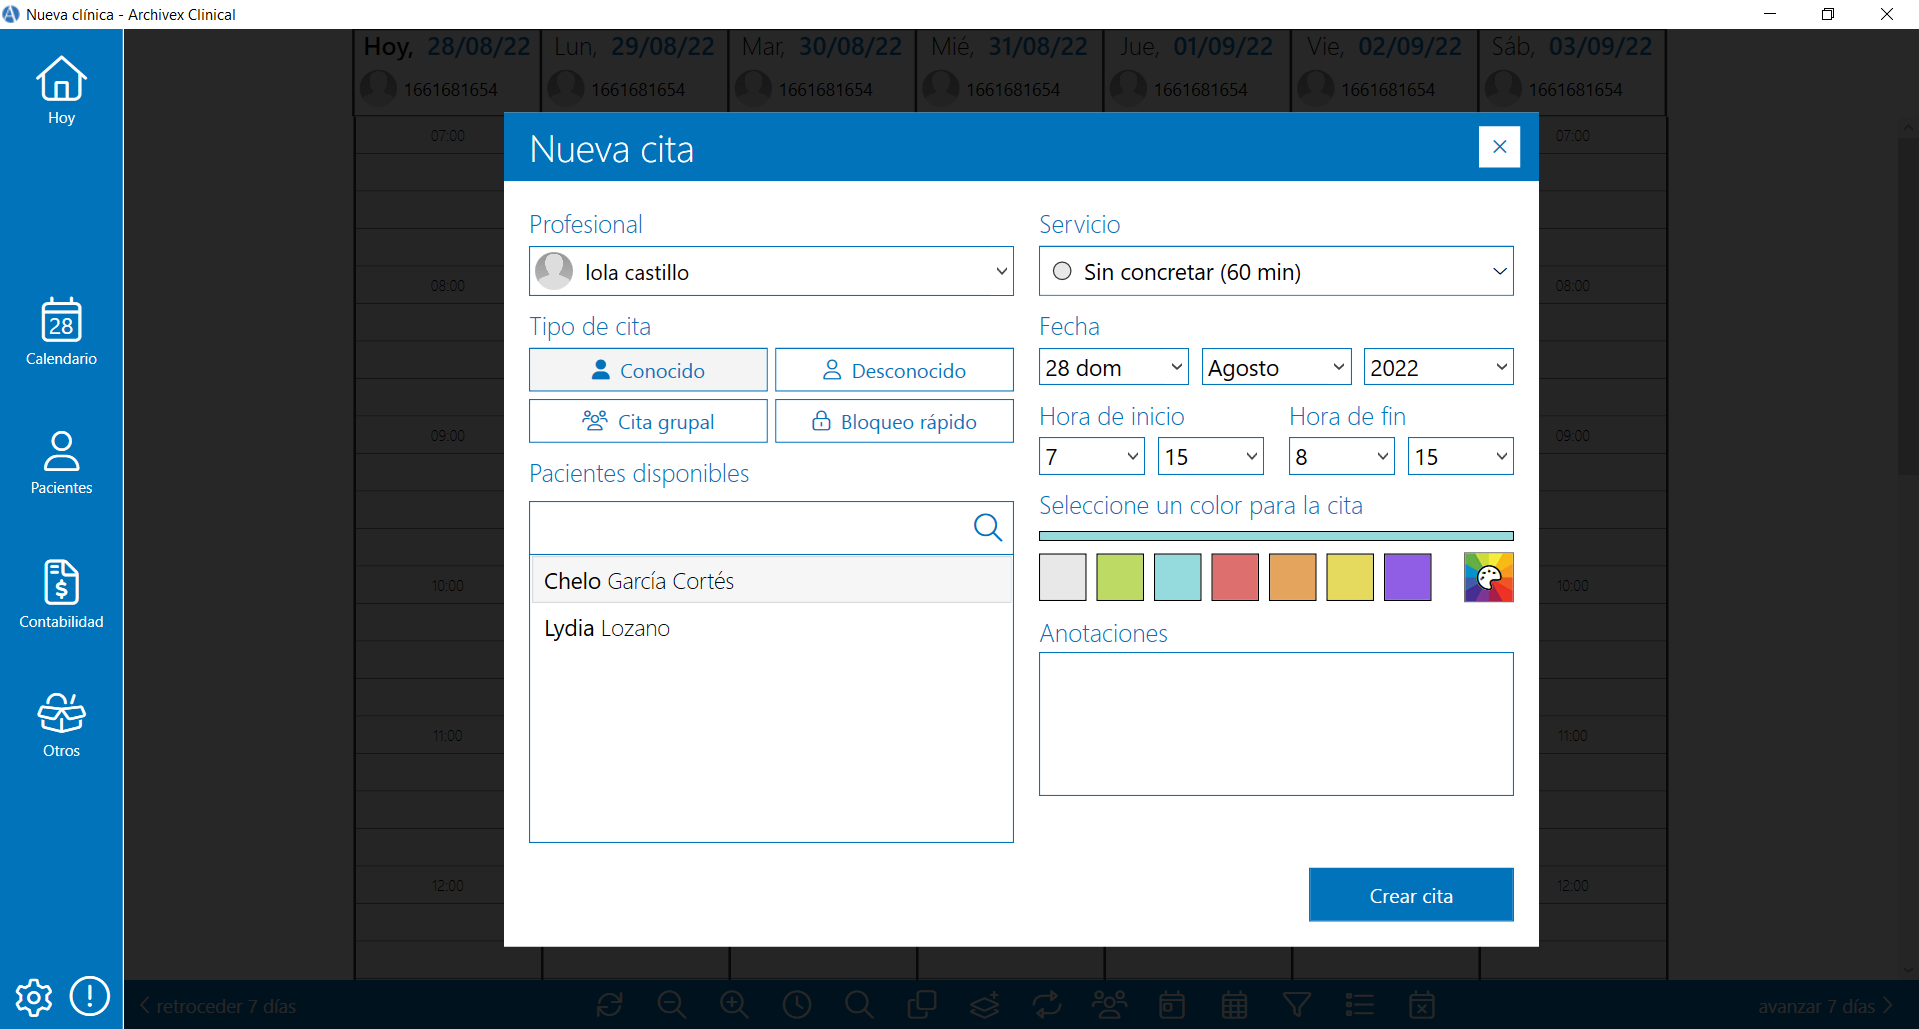
\includegraphics[scale=0.3]{doc/imagenes/archivex-crear-cita.png
    }}
    \caption{Formulario de creación de citas en Archivex}
    \label{fig:archivex-crear-citas}
\end{figure}

En conclusión después de este análisis, Archivex es un software que sería ideal por el precio y servicios ofertados para clínicas de tamaño pequeño/mediano como Carmen Verdejo contratando el Plan M o Plan L y cumpliría con su palabra de ahorro de tiempo a largo plazo cuando sus usuarios se familiarizasen más con la aplicación ya que está claro que dista de ser totalmente intuitiva. \bigskip


	% Estado del arte
	\chapter{Gestión y planificación}

\section{Metodología de desarrollo}
Es bien sabido que en el ámbito del desarrollo software durante décadas se han dado problemas como el no cumplimiento ni de requisitos, ni de estimaciones de tiempo y recursos. Son el surgimiento de estos problemas a lo que evocó a la creación de metodologías de desarrollo con el objetivo de evitar o minimizar dichos problemas. Así que, una \textbf{metodología de desarrollo} se define como un de marco de trabajo utilizado con el fin de estructurar y controlar un proceso de desarrollo. \bigskip

A continuación se muestra una tabla con los dos grupos en los que puede ser una metodología de desarrollo clasificada junto con sus respectivas diferencias:

\begin{table}[H]
\begin{tabular}{|l|l|}
\hline
\rowcolor[HTML]{EFEFEF} 
\multicolumn{1}{|c|}{\cellcolor[HTML]{EFEFEF}Metodologías tradicionales}                                                                              & \multicolumn{1}{c|}{\cellcolor[HTML]{EFEFEF}Metodologías ágiles}                                               \\ \hline
\begin{tabular}[c]{@{}l@{}}La fase de test de la aplicación \\ es realizada sólo una vez tras \\ ser la fase de desarrollo \\ completada\end{tabular} & \begin{tabular}[c]{@{}l@{}}La fase de test de la aplicación\\ es un proceso realizado de \\ forma iterativa\end{tabular} \\ \hline
Sigue una organización lineal                                                                                                                         & Sigue una organización iterativa                                                                               \\ \hline
\begin{tabular}[c]{@{}l@{}}La participación del cliente\\ es menor\end{tabular}                                                                       & La participación del cliente es mayor                                                                          \\ \hline
\begin{tabular}[c]{@{}l@{}}Apoya un modelo de desarrollo\\ fijo\end{tabular}                                                                          & \begin{tabular}[c]{@{}l@{}}Apoya un modelo de desarrollo \\adaptable al cambio\end{tabular}                    \\ \hline
Difícil la adaptación al cambio                                                                                                                       & Fácil adaptación al cambio                                                                                     \\ \hline
Gestión de equipo grandes                                                                                                                             & Gestión de equipos pequeños                                                                                    \\ \hline
\end{tabular}
\label{tabla-metodologias}
\caption{Tabla de diferencias entre metodologías de desarrollo tradicional y ágil}
\end{table}

En lo que respecta a este proyecto, se reunen varios factores para inclinarnos por las metodologías ágiles:
\begin{itemize}
    \item El proyecto va dirigido a un cliente real, el cual puede añadir, modificar o eliminar cualquier requisito de los inicialmente planteados. Por tanto, hay que estar preparado para cualquier tipo de cambio.
    \item Se pretende hacer uso de tecnologías en las que no se tiene ninguna experiencia previa y esto puede conllevar a la ralentización de la planificación y en consecuencia a llevar a cabo modificaciones en ella.
    \item Como se indica en la Tabla \ref{tabla-metodologias} las metodologías ágiles son preferibles en equipos pequeños, estando en este caso el equipo formado por una sóla persona.
\end{itemize}

Una vez escogido el tipo de metodología, dentro de las metodologías ágiles nos encontramos con un amplio abanico de marcos de trabajo: SCRUM, eXtreme Programming, Kanban, Crystal Clear,etc. Se han tenido en consideración las dos primeras ya que de acuerdo al artículo \textit{''Organizational issues in embracing Agile methods: an empirical assessment''} de Alok Mishra et al. \cite{mishra2021organizational} las dos metodologías ágiles más populares actualmente son Scrum y eXtreme Programming y en consecuencia esto significa que han sido mayormente testeadas en distintas empresas y hay una mayor cantidad de documentación sobre ellas. Teniendo en cuenta la comparativa realizada por Juan Camilo Salazar et al. \cite{salazar2018scrum} de SCRUM y XP la poca disponibilidad del cliente, el tiempo de tan sólo 3 meses del que se dispone, la posible aparición de los riesgos expuestos en la Sección \ref{riesgos}  se concluye que XP resulta muy poco viable para este proyecto, no sólo por su poca flexibilidad, sino también porque requiere de trabajo en pareja y en este proyecto sólo participa una persona. Así pues, SCRUM es el marco de trabajo ideal para la naturaleza de este proyecto. \bigskip

En la siguiente Sección \ref{scrum} se explica de forma detallada qué es SCRUM y su adaptación al proyecto.

\subsection{SCRUM} \label{scrum}

\begin{figure}[H]
    \centering{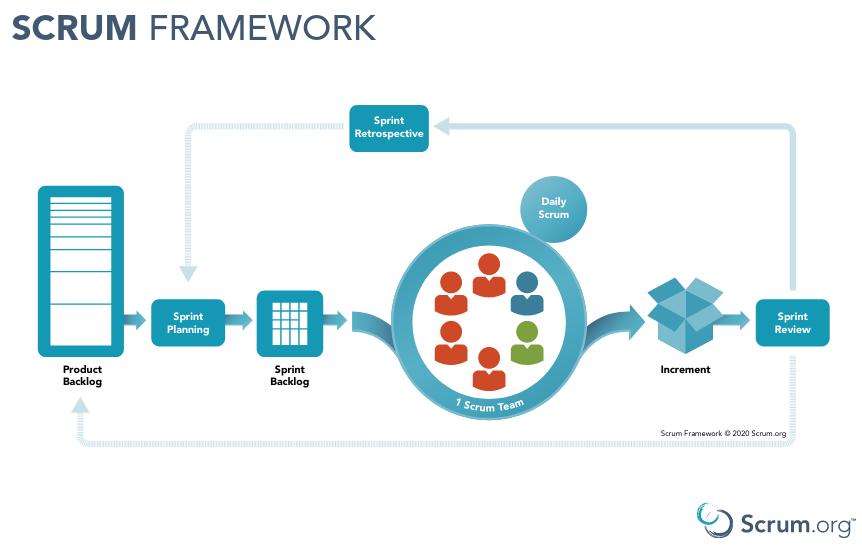
\includegraphics[scale=0.3]{doc/imagenes/scrum-esquema.png}}
    \caption{Esquema del marco de trabajo de SCRUM}
    \label{fig:scrum-esquema}
\end{figure}

La metodología de desarrollo ágil SCRUM (Figura \ref{fig:scrum-esquema}, imagen tomada de scrum.org \footnote{\url{https://www.scrum.org/}}), es de las metodologías de desarrollo más utilizadas en la actualidad, de hecho empresas de gran calibre como Movistar, Google, Vodafone, Electronic Arts... utilizan dicha metodología. \bigskip

Siguiendo el libro de Alonso Álvarez García et al. ''Métodos ágiles y Scrum'' \cite{Gomez2017-id}, ¿qué es SCRUM? Es un marco de trabajo para el desarrollo de proyecto caracterizado por ser iterativo e incremental, así como adaptativo pues no sigue un plan lineal, sino una adaptación continua. Sus principios son la \textbf{transparencia}, la \textbf{inspección} y la \textbf{adaptación} cumpliendo con los valores de mejora continua, compromiso, calidad, simplicidad, respeto, coraje, ritmo y responsabilidad. \bigskip

Sabiendo previamente que un \textbf{Sprint} es un intervalo de tiempo comprendido entre 1 a 4 semanas, durante el que se crea un incremento del producto del proyecto ''terminado'' y utilizable, SCRUM se compone de los siguientes elementos:

\begin{itemize}
    \item \textbf{Artefactos}:
    \begin{itemize}
        \item \textbf{Pila del producto (Product Backlog)}: Es una lista de requisitos que ha sido priorizada de todas las funcionalidades y características que ha de cumplir el producto. 
        \item \textbf{Pila del Sprint (Sprint Backlog)}: Es la selección de requisitos de la Pila del Producto, se compone de tareas de desarrollo que expresan los requisitos en lenguaje técnico.
    \end{itemize}
    \item \textbf{Reuniones}:
    \begin{itemize}
        \item \textbf{Planificación del Sprint}: Es una reunión previa antes del comienzo del Sprint en la que se determina el objetivo de éste y las tareas a desarrollar.
        \item \textbf{Reunión diaria}: Se trata de una reunión realizada diariamente en la que cada miembro del equipo expone las tareas realizadas, así como los obstáculos encontrados.
        \item \textbf{Revisión del Sprint}: Es una reunión que tiene lugar el último día del Sprint cuyo objetivo es el de obtener información sobre el estado del proyecto.
        \item \textbf{Retrospectiva del Sprint}: Al final de cada Sprint se realiza una reunión de retrospectiva en la que se identifican los puntos fuertes a mantener y débiles a mejorar del equipo durante el desarrollo.
    \end{itemize}
    \item \textbf{Roles}:
        \begin{itemize}
        \item \textbf{Propietario}: Es el representante del cliente, debe de conocer los requisitos del cliente y tener cierta experiencia con los métodos utilizados por el equipo. Se encarga de recolectar los requisitos del cliente, resolver dudas del Equipo de Desarrollo y de priorizar la Pila del Producto, así como de aceptar o rechazar el software realizado al final una iteración.
        \item \textbf{Director del proyecto}: Promueve los valores de Scrum, se asegura de que el equipo es totalmente funcional y es su escudo del resto del equipo ante amenazas externas. Se encarga de asegurar que el Propietario conozca cómo ordenar la Pila del Producto para maximizar el valor, de guiar y ayudar al Equipo de Desarrollo y motivar a que se realicen cambios que incrementen la productividad.
        \item \textbf{Equipo de desarrollo}: Se forma por un conjunto de profesionales que se ocupan de entregar un incremento del producto del proyecto ''terminado'' al final de cada Sprint. Normalmente un Equipo de Desarrollo se forma entre 5-9 personas.
    \end{itemize}
\end{itemize}

\subsection{Aplicación de SCRUM a este proyecto}
Debido a que el desarrollo del proyecto se hará de forma individual, se debe de hacer una adaptación de SCRUM a la metodología de trabajo que se va a llevar a lo largo del proyecto.

\begin{itemize}
    \item Como el Equipo de Desarrollo está compuesto por una sóla persona, las reuniones diaras son eliminadas.
    \item Al final de cada Sprint se acordará una reunión con la tutora en la que se hará una retrospectiva de éste. Además, durante todo el desarrollo se mantendrá el contacto para posibles dificultades o dudas.
\end{itemize}

\subsection{Especificación de requisitos}
En todo proyecto de desarrollo de un producto software es crucial una buena definición de los requisitos que deberá de cumplir éste para satisfacer totalmente las necesidades de sus usuarios. Debido a que como se ha explicado con anterioridad se está siguiendo la metodología de desarrollo ágil SCRUM, la definición de requisitos se hará a partir de historias de usuario. \bigskip

A continuación se muestran las historias de usuario identificadas para el desarrollo del proyecto. Cabe mencionar que, debido a su complejidad, las historias de usuario 2 (Tabla \ref{HU2}) y 3 (Tabla \ref{HU3}) han sido desglosadas en ''sub-historias de usuario''. 

\begin{table}[H]
\begin{tabular}{|
>{\columncolor[HTML]{CCCCCC}}l |l|}
\hline
\textbf{Identificación} & HU.1 - Sistema de inicio de sesión\\ \hline
\textbf{Descripción}    & Como usuario quiero poder iniciar y cerrar sesión de la plataforma. \\ \hline
\textbf{Aceptación}     & \begin{tabular}[c]{@{}l@{}}- El usuario intenta iniciar sesión, pero no está registrado \\ o las credenciales introducidas son erróneas y el sistema informa \\ de dicho error por la interfaz.\\ - Un usuario registrado introduce correctamente sus crendenciales y \\ es redirigido a la vista principal de la plataforma \\ obteniendo un JWT con fecha de expiración.\end{tabular}
\\ \hline
\textbf{Prioridad}     & \begin{tabular}[c]{@{}l@{}}Alta\end{tabular} \\ \hline
\textbf{Estimación}     & \begin{tabular}[c]{@{}l@{}}2 semanas\end{tabular} \\ 
\\ \hline\textbf{Tareas} & \begin{tabular}[c]{@{}l@{}}- Investigación sobre cómo implementar un sistema de login.\\ - Definir y crear el modelo de la base de datos de los usuarios.\\ - Definir un sistema jerárquico de roles.\\ - Implementar en Backend un sistema de login.\\ - Diseñar la interfaz del login.\\ - Implementar el diseño realizado en Frontend e implementar \\ las llamadas necesarias al Backend.\end{tabular} \\ \hline
\end{tabular}
\caption{HU.1 - Sistema de inicio de sesión}
\end{table}
\clearpage
\begin{table}[H]
\begin{tabular}{|
>{\columncolor[HTML]{CCCCCC}}l |l|}
\hline
\textbf{Identificación} & HU.2- Gestionar citas de un usuario \\ \hline
\textbf{Descripción}    & Como usuario quiero visualizar, crear, editar y borrar citas.  \\ \hline
\textbf{Aceptación}     & \begin{tabular}[c]{@{}l@{}}- Un usuario accede a la vista del ''Calendario'' y \\ visualiza las citas en las que éste dispone de permisos \\ para realizar cualquier operación CRUD.\end{tabular}         \\ \hline
\textbf{Prioridad}     & \begin{tabular}[c]{@{}l@{}}Alta\end{tabular} \\ \hline
\textbf{Estimación}     & \begin{tabular}[c]{@{}l@{}}2 semanas\end{tabular} \\ \hline 
\textbf{Tareas}         & \begin{tabular}[c]{@{}l@{}}- Investigación de Angular Schedule.\\ - Definir y crear el modelo de la base de datos de las citas.\\ - Diseñar la interfaz de la vista principal.\\ - Implementar los endpoints para operaciones CRUD sobre \\ citas en Backend utilizando el modelo de datos de Angular Schedule.\\ - Implementar el diseño realizado e implementar las llamadas a Backend.\end{tabular} \\ \hline
\end{tabular}
\caption{HU.2 - Gestionar citas de un usuario}
\label{HU2}
\end{table}

\begin{table}[H]
\begin{tabular}{|
>{\columncolor[HTML]{CCCCCC}}l |l|}
\hline
\textbf{Identificación} & HU.2.1- Visualización de las citas en el calendario  \\ \hline
\textbf{Descripción}    & \begin{tabular}[c]{@{}l@{}}Como usuario quiero visualizar en un calendario las \\ próximas citas y las pasadas.\end{tabular}  \\ \hline
\textbf{Prioridad}     & \begin{tabular}[c]{@{}l@{}}Alta\end{tabular} \\ \hline
\textbf{Estimación}     & \begin{tabular}[c]{@{}l@{}}1 semana\end{tabular} \\ \hline 
\textbf{Aceptación}     & \begin{tabular}[c]{@{}l@{}}- Un usuario paciente entra a la vista de ''Calendario'' y \\ visualiza todas sus citas en \\ un calendario.\\ - Un usuario psicólogo entra a la vista de ''Calendario'' y \\ visualiza todas las citas\\ de sus pacientes en un calendario.\\ - Un usuario administrador entra a la vista ''Calendario'' y \\ visualiza todas las citas de todos los usuarios en un calendario.\\ - Un usuario pulsa sobre una cita y el diálogo aparece \\ con todos los campos rellenos asociados a esa cita.\end{tabular} \\ \hline
\textbf{Tareas} & \begin{tabular}[c]{@{}l@{}}- Investigación de Angular Schedule\\ - Definir y crear el modelo de la base de datos de las citas\\ - Diseñar la interfaz de la vista del calendario\\ - Implementar el diseño realizado\end{tabular}  \\ \hline
\end{tabular}
\caption{HU.2.1 - Visualización de las citas en el calendario}
\end{table}

\begin{table}[H]
\begin{tabular}{|
>{\columncolor[HTML]{CCCCCC}}l |l|}
\hline
\textbf{Identificación} & HU.2.2- Crear y editar una cita \\ \hline
\textbf{Descripción}    & Como usuario quiero crear y modificar una cita en el calendario \\ \hline
\textbf{Prioridad}     & \begin{tabular}[c]{@{}l@{}}Alta\end{tabular} \\ \hline
\textbf{Estimación}     & \begin{tabular}[c]{@{}l@{}}1 semana\end{tabular} \\ \hline 
\textbf{Aceptación}     & \begin{tabular}[c]{@{}l@{}}- Un usuario pulsa sobre la franja de un día del calendario \\ y se abre un diálogo con un formulario con los campos: paciente, \\ psicólogo, hora de inicio de la cita, hora de fin de la cita y observaciones.\\ - Un usuario paciente intenta editar los campos de paciente con \\ su nombre y psicólogo con el nombre de su psicólogo, pero no puede \\ porque está deshabilitado.\\ - Un usuario psicólogo intenta editar el campo de psicólogo con su \\ nombre, pero no puede porque está deshabilitado.\\ - Un usuario administrador intenta modificar todos los campos y estos \\ son modificados con éxito.\\ - Un usuario intenta modificar el día y/u hora mostrados de la cita con un \\ especialista a una cita que no se encuentra libre, se muestra un \\ mensaje informado de ello.\\ - Se pulsa sobre el botón de guardado, el diálogo se cierra y una nueva cita \\ aparece en el calendario.\\ - Se pulsa sobre el botón de ''Cancelar'' y el diálogo se cierra.\end{tabular} \\ \hline
\textbf{Tareas}         & \begin{tabular}[c]{@{}l@{}}- Implementar los endpoints crear y editar citas en Backend \\ utilizando el modelo de datos de Angular Schedule.\\ - Implementar las llamadas a Backend en Frontend.\\ - Implementar el diálogo de creación/edición de citas en Frontend.\end{tabular}      \\ \hline
\end{tabular}
\caption{HU.2.2 - Crear y editar una cita }
\end{table}

\begin{table}[h]
\begin{tabular}{|
>{\columncolor[HTML]{CCCCCC}}l |l|}
\hline
\textbf{Identificación} & HU.2.3- Eliminar las citas de un usuario \\ \hline
\textbf{Descripción}    & Como usuario quiero eliminar una cita  \\ \hline
\textbf{Prioridad}     & \begin{tabular}[c]{@{}l@{}}Alta\end{tabular} \\ \hline
\textbf{Estimación}     & \begin{tabular}[c]{@{}l@{}}1 día\end{tabular} \\ \hline 
\textbf{Aceptación}     & \begin{tabular}[c]{@{}l@{}}- Se pulsa el botón de borrado de una cita existente, \\ se abre un diálogo preguntando si el usuario está seguro de la \\ acción, pulsa sí, el diálogo se cierra y ésta es eliminada del calendario.\\ - Se pulsa el botón de borrado de una cita existente, se abre un\\ diálogo preguntando si el usuario está seguro de la acción, pulsa no \\ y el diálogo se cierra sin tener efecto alguno.\end{tabular} \\ \hline
\textbf{Tareas}         & \begin{tabular}[c]{@{}l@{}}- Implementar el endpoint para eliminar citas en Backend.\\ - Implementar las llamadas a Backend en Frontend.\\ - Implementar el diálogo para confirmar el borrado de una cita en Frontend.\end{tabular} \\ \hline
\end{tabular}
\caption{HU.2.3 - Eliminar las citas de un usuario }
\end{table}

\begin{table}[H]
\begin{tabular}{|
>{\columncolor[HTML]{CCCCCC}}l |l|}
\hline
\textbf{Identificación} & HU.3- Gestión de los usuarios de la plataforma  \\ \hline
\textbf{Descripción}    & \begin{tabular}[c]{@{}l@{}}Como administrador quiero poder consultar, añadir, \\ modifcar y borrar usuarios de la plataforma.\end{tabular}                \\ 
\hline
\textbf{Prioridad}     & \begin{tabular}[c]{@{}l@{}}Alta\end{tabular} \\ \hline
\textbf{Estimación}     & \begin{tabular}[c]{@{}l@{}}2 semanas\end{tabular} \\ \hline 
\textbf{Aceptación}     & \begin{tabular}[c]{@{}l@{}}· Al pulsar sobre la sección de ''Pacientes'' del menú lateral, se navegará a una \\ nueva vista en la que se mostrará un listado de los pacientes de la clínica.\\ · Al pulsar sobre la sección de "Psicólogos" del menú lateral, \\ se navegará a una nueva vista en la que se mostrará un listado \\ de los psicólogos de la clínica.\\ ·Al pulsar sobre el botón de editar se mostrará un diálogo \\ con los campos del usuario a editar.\\ · Un campo del diálogo de editar un usuario se deja en \\ blanco y se informa del error.\\ · Todos los campos están rellenados y se pulsa sobre el botón \\ de guardado, el diálogo se cierra y la información del usuario \\ queda actualizada.\\ · Se pulsa sobre el botón de cancelar del diálogo y éste se cierra \\ sin haberse producido ningún efecto en la información del usuario.\\ · Se pulsa sobre el botón de eliminar, un diálogo es mostrado \\ preguntando si el usuario está seguro de dicha acción, se pulsa sí, el diálogo\\  se cierra y el usuario seleccionado es eliminado del listado, así como sus citas.\\ · Se pulsa sobre el botón de eliminar, un diálogo es mostrado\\  preguntando si el usuario está seguro de dicha acción, se pulsa ''Cancelar'' \\ y el diálogo se cierra sin tener ningún efecto.\end{tabular} \\ \hline
\textbf{Tareas}         & \begin{tabular}[c]{@{}l@{}}· Implementación de endpoints CRUD para los usuarios de la plataforma.\\ · Diseñar la vista del listado del personal\\ · Diseñar la vista del listado de pacientes.\\ · Implementar los diseños de las vistas anteriores.\end{tabular}            \\ \hline
\end{tabular}
\caption{HU.3- Gestión de los usuarios de la plataforma }
\label{HU3}
\end{table}

\begin{table}[H]
\begin{tabular}{|
>{\columncolor[HTML]{CCCCCC}}l |l|}
\hline
\textbf{Identificación} & HU.3.1- Crear y editar usuarios en la plataforma               \\ \hline
\textbf{Descripción}    & \begin{tabular}[c]{@{}l@{}}Como administrador quiero poder consultar, añadir, \\ modifcar y borrar usuarios de la \\ plataforma.\end{tabular}      \\ \hline
\textbf{Prioridad}     & \begin{tabular}[c]{@{}l@{}}Alta\end{tabular} \\ \hline
\textbf{Estimación}     & \begin{tabular}[c]{@{}l@{}}1 semana\end{tabular} \\ \hline 
\textbf{Aceptación}     & \begin{tabular}[c]{@{}l@{}}- Al pulsar sobre el botón de crear usuario se mostrará \\ un diálogo con todos los campos asociados a un usuario.\\ - Al pulsar sobre el botón de editar se mostrará un diálogo \\ con los campos del usuario a editar.\\ - Un campo del diálogo de editar un usuario se deja en blanco \\ y se informa del error.\\ - Todos los campos están rellenados y se pulsa sobre el botón de \\ guardado, el diálogo se cierra y la información del usuario \\ queda actualizada.\\ - Se pulsa sobre el botón de cancelar del diálogo y éste se cierra \\ sin haberse producido ningún efecto en la información del usuario.\end{tabular} \\ \hline
\textbf{Tareas}         & \begin{tabular}[c]{@{}l@{}}- Implementación de endpoints para crear y \\ editar usuarios en la plataforma.\\ - Implementar las llamadas en Front al Backend \\ para crear y editar usuarios.\end{tabular}    \\ \hline
\end{tabular}
\caption{HU.3.1 - Crear y editar usuarios en la plataforma  }
\end{table}

\begin{table}[H]
\begin{tabular}{|
>{\columncolor[HTML]{CCCCCC}}l |l|}
\hline
\textbf{Identificación} & HU.3.2- Borrar usuarios de la plataforma \\ \hline
\textbf{Descripción}    & \begin{tabular}[c]{@{}l@{}}Como administrador quiero poder borrar usuarios de la \\ plataforma.\end{tabular}  \\ \hline
\textbf{Prioridad}     & \begin{tabular}[c]{@{}l@{}}Alta\end{tabular} \\ \hline
\textbf{Estimación}     & \begin{tabular}[c]{@{}l@{}}1 semana\end{tabular} \\ \hline 
\textbf{Aceptación}     & \begin{tabular}[c]{@{}l@{}}- Se pulsa sobre el botón de eliminar, un diálogo es \\ mostrado preguntando si el usuario está seguro de \\ dicha acción, se pulsa sí, el diálogo se cierra y el \\ usuario seleccionado es eliminado del listado. \\ - Se pulsa sobre el botón de eliminar, un diálogo es \\ mostrado preguntando si el usuario está seguro de dicha \\ acción, se pulsa ''Cancelar'' y el diálogo se cierra sin \\ tener ningún efecto.\end{tabular} \\ \hline
\textbf{Tareas}         & \begin{tabular}[c]{@{}l@{}}- Implementación del endpoint encargado de borrar \\ usuarios de la plataforma.\\ - Implementar la llamada al endpoint para eliminar \\ usuarios en Frontend\end{tabular}    \\ \hline
\end{tabular}
\caption{HU.3.2 - Borrar usuarios de la plataforma }
\end{table}

\begin{table}[H]
\begin{tabular}{|
>{\columncolor[HTML]{CCCCCC}}l |l|}
\hline
\textbf{Identificación} & HU.4- Gestionar el perfil de un usuario \\ \hline
\textbf{Descripción}    & Como usuario quiero gestionar mi perfil de la plataforma \\ 
\hline
\textbf{Prioridad}     & \begin{tabular}[c]{@{}l@{}}Media\end{tabular} \\ \hline
\textbf{Estimación}     & \begin{tabular}[c]{@{}l@{}}2 semanas\end{tabular} \\ \hline 
\textbf{Aceptación}     & \begin{tabular}[c]{@{}l@{}}- Al pulsar sobre la opción de ''Perfil'' del menú lateral \\ se abre un diálogo en el que se muestran el email, nombre \\, rol del usuario es mostrado y un formulario para cambiar la contraseña actual.\\ - El usuario intenta pulsar sobre rol pero no puede editarlo.\\ - El usuario intenta pulsar sobre email o nombre y el campo es editable.\\. El usuario introduce la nueva contraseña, pulsa \\ sobre el botón de guardardado y la contraseña es actualizada.\\ - El usuario pulsa sobre cambiar contraseña y un diálogo es mostrado \\ con un formulario para introducir su contraseña actual y la nueva. \end{tabular} \\ \hline
\textbf{Tareas}         & \begin{tabular}[c]{@{}l@{}}- Diseñar la vista de
perfil\\ -  Añadir endpoint para cambiar
la contraseña de un usuario en
backend\\ - Implementar en Frontend el diseño realizado\end{tabular}  \\ \hline
\end{tabular}
\caption{HU.4 - Gestionar el perfil de un usuario  }
\end{table}


\subsection{Requisitos adicionales}
\begin{itemize}
    \item \textbf{Usabilidad}: La plataforma deberá de ser intuitiva, con flujos de usuario sencillos.
    \item \textbf{Seguridad}: La plataforma deberá de garantizar la privacidad de los datos proporcionados por los usuarios.
    \item \textbf{Compatibilidad}: El código podrá ser portable y funcionar correctamente en cualquier sistema operativo.
    \item \textbf{Costo}: Se procurará que el coste del proyecto sea el más bajo posible
    \item \textbf{Mantenimiento}: Para su posterior mantenimiento las partes de código más complejas deberán de haber sido comentadas.
\end{itemize}{}


\section{Gestión de la configuración}
En esta sección se indicará cómo se procederá para la gestión de la configuración de todos los elementos pertenecientes a este proyecto. Debido a que los elementos de trabajo que conforman el proyecto son el código y la documentación, a continuación se explicará la gestión de cada uno por separado.

\subsection{Gestión del código}
Para la gestión del código, control de versines del mismo y para evitar cualquier posible pérdida se hará uso de Github y de Git. Para ello, se procederá a crear un repositorio en local vinculado al repositorio en remoto de Github que previamente habrá sido creado con el nombre \textbf{TFG}\footnote{\url{https://github.com/ins426/TFG}}. En el \textit{README} \footnote{\url{https://github.com/ins426/TFG#bachelors-thesis-dayday-appointment-scheduling-for-clinics}} de dicho repositorio se encontrarán los enlaces a los dos repositorios que contendrán el código de la plataforma, uno para el backend llamado \textbf{TFG-backend} \footnote{\url{https://github.com/ins426/TFG-backend}} y otro para el frontend llamado \textbf{TFG-frontend}\footnote{\url{https://github.com/ins426/TFG-frontend}}. Al igual que con el repositorio global, también se tendrá un repositorio en local para cada uno. \bigskip

En cuanto a las herramientas utilizadas en cada repositorio, el backend será implementado en el lenguaje de programación JavaScript haciendo uso de Node.js y Express para construir la API. Por otro lado, el frontend será implementado en el lenguaje TypeScript haciendo uso de Angular y se utilizarán HTML, SCSS, Angular Material, Angular Flex-Layout y RxJS para construir la interfaz. \bigskip

Todas las herramientas mencionadas anteriormente son más adelante explicadas en la Sección \ref{recursos-software}.

\subsection{Gestión de la documentación}
En lo que respecta a la gestión de la documentación, ésta será redactada en la plataforma Overleaf en LaTeX y cada entrega realizada a la tutora será alojada en el repositorio \textit{TFG} de Github del proyecto. Debido a que Overleaf requiere de un plan de pago para llevar a cabo la sincronización con Github, se ha utilizado el repositorio en local creado para llevar a cabo dicha sincronización con el repositorio en remoto.

\section{Gestión del tiempo} \label{gestion-tiempo}
Para alcanzar con los objetivos propuestos del proyecto se han definido una serie de épicas y tareas asociadas a ellas:
\begin{itemize}
    \item \textbf{E.1} Estado del arte de la gestión de citas online:
    \begin{itemize}
        \item \textbf{T.1.1}: Entrevista con la clínica Carmen Verdejo para conocer su gestión actual de citas.
        \item \textbf{T.1.2}: Investigación sobre las herramientas utilizadas en la clínica Carmen Verdejo.
        \item \textbf{T.1.3}: Buscar y leer literatura sobre gestión de citas online.
        \item \textbf{T.1.4}: Investigación de soluciones genéricas dedicadas a planificación.
        \item \textbf{T.1.5}: Investigación de soluciones específicas para la gestión de citas en centros sanitarios.
    \end{itemize}
    
    \item \textbf{E.2}: Implementación de un login para personal y pacientes:
    \begin{itemize}
        \item \textbf{T.2.1}: Investigación sobre cómo implementar un sistema de login.
        \item \textbf{T.2.2}: Definir y crear el modelo de la base de datos de los usuarios.
        \item \textbf{T.2.3}: Definir un sistema jerárquico de roles.
        \item \textbf{T.2.4}: Implementar en Backend un sistema de login.
        \item \textbf{T.2.5}: Diseñar la interfaz del login.
        \item \textbf{T.2.6}: Implementar el diseño realizado en T.2.3 en Frontend e implementar las llamadas al Backend.
    \end{itemize}
    
    \item \textbf{E.3}: Implementación de la vista principal:
    \begin{itemize}
        \item \textbf{T.3.1}: Investigar Angular Schedule de Syncfusion.
        \item \textbf{T.3.2}: Definir y crear el modelo de la base de datos de las citas.
        \item \textbf{T.3.3}: Diseñar la interfaz de la vista del calendario.
        \item \textbf{T.3.4}: Implementar el diseño realizado.
        \item \textbf{T.3.5}:  Implementar los endpoints crear y editar citas en Backend utilizando el modelo de datos de Angular Schedule de Syncfusion.
        \item \textbf{T.3.6}: Implementar las llamadas de creación y edición de citas a Backend en Frontend.
        \item \textbf{T.3.7}:  Implementar el diálogo de creación/edición de citas en Frontend.
        \item \textbf{T.3.8}: Implementar el endpoint para eliminar citas en Backend.
        \item \textbf{T.3.9}: Implementar el diálogo para confirmar el borrado de una cita en Frontend.
    \end{itemize}
    \item \textbf{E.4}: Implementación de las vistas del listado de personal y pacientes:
    \begin{itemize}
        \item \textbf{T.4.1}:  Implementación de endpoints para creación y edición de usuarios de la plataforma.
        \item \textbf{T.4.2}: Diseñar la vista del listado del personal y pacientes.
        \item \textbf{T.4.3}: Implementar las llamadas en frontend al backend para crear y editar usuarios.
        \item \textbf{T.4.4}: Implementar las vistas de los diseños de T.4.2.
        \item \textbf{T.4.5}: Implementar el endpoint encargado de borrar usuarios de la plataforma.
        \item \textbf{T.4.6}: Implementar la llamada al endpoint para eliminar usuario en Frontend.
    \end{itemize}
    \item \textbf{E.5}: Implementación de la vista de perfil:
    \begin{itemize}
        \item \textbf{T.5.1}: Diseñar la vista de perfil.
        \item \textbf{T.5.2}: Añadir endpoint de cambiar contraseña en el Backend.
        \item \textbf{T.5.3}: Implementar en Frontend el diseño de T.5.1. y conectarlo con el Backend
    \end{itemize}

    \item \textbf{E.6}: Implementación de pruebas:
    \begin{itemize}
        \item \textbf{T.6.1}: Hacer estudio de tecnologías para realizar las pruebas.
        \item \textbf{T.6.2}: Definición e implementación de las pruebas.
    \end{itemize}   

\end{itemize}

\subsection{Planificación temporal}
En el siguiente Diagrama de Gantt (Figura \ref{fig:gantt}) se recoge la temporización estimada del proyecto:

\begin{figure}[H]
    \centering{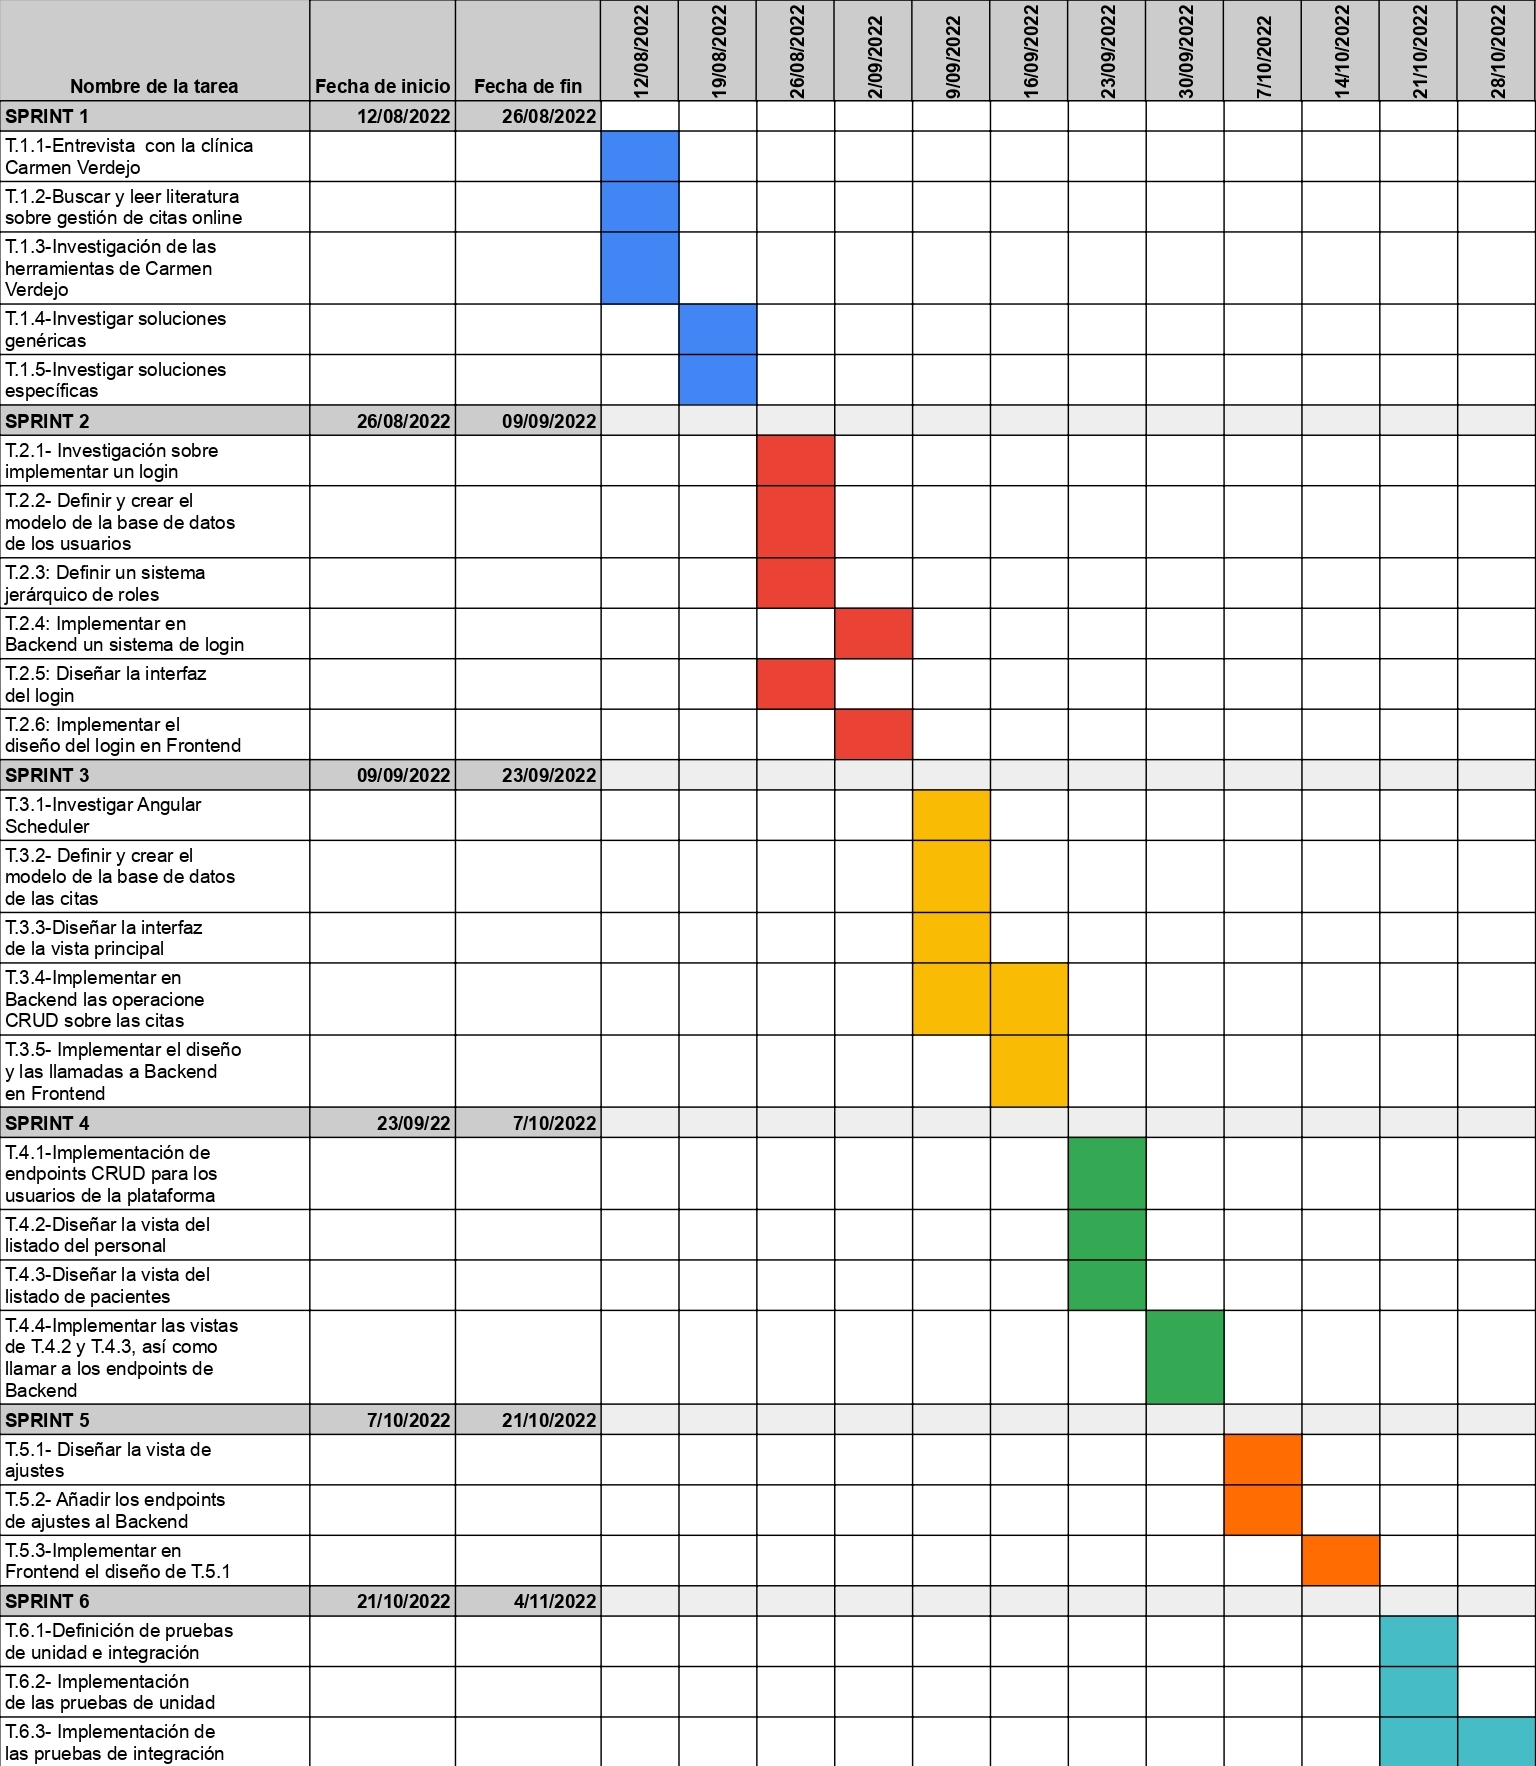
\includegraphics[scale=0.47]{doc/imagenes/gantt.jpg
    }}
    \caption{Diagrama de Gantt de la planificación temporal}
    \label{fig:gantt}
\end{figure}

Además de estas tareas, durante el desarrollo del proyecto se redactará toda la documentación correspondiente a éste.

\section{Gestión de recursos} \label{recursos}
\subsection{Recursos humanos}
\begin{itemize}
    \item \textbf{Dña. Rocío Celeste Romero Zaliz}, profesora del Departamento de Ciencias de la Computación e Inteligencia Artificial de la Universidad de Granada como tutora del proyecto.
    \item \textbf{Inés Nieto Sánchez}, estudiante del grado en Ingeniería Informática en la Escuela Técnica Superior de Ingenierías Informática y Telecomunicación.
\end{itemize}

\subsection{Recursos materiales} \label{materiales}
Los recursos utilizados para este Trabajo de Fin de Grado han sido muy pocos, en concreto sólo se ha utilizado el portátil personal:
\begin{itemize}
    \item \textbf{MSI Modern 14 A10M}: Se trata de un portatil de la marca MSI con un procesador Comet Lake i7-10510U con una memoria RAM de 16GB y una arquitectura de 64 bits. Todo el desarrollo del proyecto, así como la documentación correspondientes serán realizados haciendo uso de este portátil.
\end{itemize}
\subsection{Recursos software} \label{recursos-software}
En cuanto a los recursos software se ha optado por la utilización de software de código abierto y recurrido a las licencias gratuitas ofrecidas al estudiantado para disminuir lo máximo posible el coste del proyecto. A continuación se expone el listado de los recursos software utilizados:

\begin{itemize}
    \item \textbf{Elementary OS}: Se trata de una distribución de código abierto del sistema operativo Linux.
    \item \textbf{WebStorm}: Es una IDE dedicada sobretodo al desarrollo web en JavaScript y Typesrcipt. Pertenece a la empresa de desarrollo software JetBrains y a pesar de que todas las IDEs desarrolladas por JetBrains son de pago, se hará uso de la licencia gratuita ofrecida a estudiantes.
    \item \textbf{Git}: Se trata de un software de código abierto para el control de versiones de un proyecto.
    \item \textbf{Github}: Es una plataforma cuyo servicio es el de alojar el sistema de control de versión Git.
    \item \textbf{Docker}: Es una herramienta de código abierto diseñada con objeto de automatizar el despliegue de aplicaciones en contenedores software.
    \item \textbf{Docker Compose}: Es una herramienta dedicada a la orquestación de contenedores Docker.
    \item \textbf{Node.js}: Es un entorno de código abierto utilizado para hacer uso de JavaScript ejecutar JavaScript fuera del navegador.
    \item \textbf{Express.js}: Se trata de un framework de código abierto de backend para aplicaciones web de Node.js para construir APIs RESTful.
    \item \textbf{Angular}: Es un framework de código abierto desarrollado por Google utilizado para crear aplicaciones web y móviles.
    \item \textbf{MongoDB Atlas}: Es un servicio sobre gestión de base de datos MongoDB basado en la nube. Se hará uso de su prueba gratis en la que se permite la creación de una base de datos gratuita. 
    \item \textbf{Postman}: Se trata de una plataforma API para construir y crear APIs. Será utilizada para probar la funcionalidad de los endpoints de la aplicación.
    \item \textbf{AWS}: Es un conjunto de servicios de computación en la nube. Se hará uso del servicio EC2 y Route 53 para hacer el despliegue. Estos servicios tienen un coste en un función de sus horas de uso. El tipo de instancia escogida que se explicará en el Capítulo \ref{despliegue} tiene un precio de 0,047€/hora. Se prevee un uso máximo de la instancia de unas 10 horas por lo que aproximadamente su coste máximo será de 0.47€.
    \item \textbf{Cloudfare}: Como la anterior herramienta, formará parte del despliegue y será utilizada para comprar un dominio para la plataforma. En este caso el dominio escogido tuvo un precio de 4€.
    \item \textbf{Let's Encrypt}: Es una autoridad de certificación que ofrece de manera gratis certificados SSL.
\end{itemize}

\subsection{Recursos  de comunicación y documentación}
Para la correcta evolución del proyecto se han de hacer uso de recursos para la comunicación entre sus participantes, así como el uso de herramientas utilizadas para la documentación del mismo.

\begin{itemize}
    \item \textbf{Overleaf}: Es un editor gratuito de LaTeX en la nube, utilizado para la documentación del proyecto.
    \item \textbf{Jira}: Software dedicado a la gestión de proyectos, se utilizará su plan grautito para la gestión del proyecto siguiendo una metodología SCRUM.
    \item \textbf{Visual Paradigm}: Es una aplicación software cuyo objetivo es el de modelado de sistemas de información y procesos de gestión de desarrollo. Se trata de una herramienta de pago, pero la Universidad de Granada ofrece a su estudiantado licencias gratuitas.
    \item \textbf{Draw.io}: Es un software online gratuito desarrollado por Google utilizado para la creación de diagramas y esquemas.
    \item \textbf{Figma}: Herramienta de diseño para crear aplicaciones, webs, logos...Su paquete gratis será utilizado para la creación de los wireframes y mockups de la plataforma.
    \item \textbf{Milanote}: Es un software gratis en la nube diseñado para organizar ideas y proyectos en tableros visuales.
    \item \textbf{Google slides}: Es una herramienta desarrollada por Google para la creación y edición de presentaciones. Será utilizada para la elaboración de la presentación del proyecto.
    \item \textbf{Google meet}: Es un servicio de videoconferencia desarrollado por Google.
    \item \textbf{Correo UGR}: Es un servicio de correo electrónico de la UGR.
    \item \textbf{Clockify}: Es una herramienta para dejar registro de las horas trabajadas en un proyecto.
\end{itemize}

\section{Gestión de costes}
En esta sección se elaborará un presupuesto de acuerdo a los recursos explicados en la Sección \ref{recursos} junto con los costes adicionales que supone el desarrollo del proyecto.

\subsection{Costes de recursos humanos}
Para los costes de recursos humanos, hemos de tener en cuenta que el equipo de desarrollo está formado por una persona que tomará el rol de Ingeniera Informática. Para estimar el coste del trabajo de dicho rol a continuación se hará un desglose del número de horas totales a trabajar y su coste. \bigskip

El proyecto se encuentra planteado para ser realizado en un período de 3 meses, es decir, 12 semanas. 

\begin{center}
$Dias\ naturales\ =\ 3\ meses\ *\ 30\ dias / mes\ =\ 90\ dias$
\end{center}

A este número de días naturales habrá que descontarle fines de semana:

\begin{center}
$Dias\ no \ laborales\ =\ 3\ meses\ *\ 8\ dias / mes\ =\ 24\ dias$
\end{center}

Resultando ser los días laborales invertidos en el desarrollo del proyecto los siguientes:

\begin{center}
$Dias\ laborales\ =\ 90\ dias\ -\ 24\ dias =\ 66 \ dias$
\end{center}

En cuanto a las horas trabajadas, una jornada laboral completa se constituye de 40 horas semanales. Sin embargo, debido a que la estudiante trabaja en paralelo con una jornada parcial durante la realización del proyecto, las horas semanales dedicadas son reducidas a 30 horas distribuidas en 6 horas diarias. Por tanto, el total de horas trabajadas es el siguiente:

\begin{center}
$Horas\ laborales\ =\ 66\ dias\ *\ 6 \ horas\ día = \ 396 \ horas$
\end{center}

Después de haber obtenido las horas laborales totales, el salario como ingeniero informático se ha obtenido en base al salario anual indicado por la Universidad Alfonso X El Sabio \footnote{\url{https://www.uax.com/blog/ingenieria/cuanto-cobra-un-ingeniero-informatico}}. Según la universidad madrileña el salario de un ingeniero informático con menos de 3 años de experiencia gana aproximadamente 20.450 euros anuales, en otras palabras, 1.704 euros mensuales brutos que son 9,68 euros/hora. Así pues los costes de recursos humanos totales son:

\begin{center}
$Costes\ de \ recursos \ humanos \ =\ 396\ horas\ *\ 9.68 \ euros\ hora = \ 3.833,28 \ euros$
\end{center}

Sin embargo, se utilizó la herramienta Clockify para hacer un registro de las horas invertidas en el proyecto (Figura \ref{fig:clockify}), que como se ve finalmente fueron 413 horas. Por ello los costes de recursos humanos reales han sido:

\begin{center}
$Costes\ de \ recursos \ humanos \ reales \ =\ 413\ horas\ *\ 9.68 \ euros\ hora = \ 3997,84 \ euros$
\end{center}

\begin{figure}[H]
    \centering{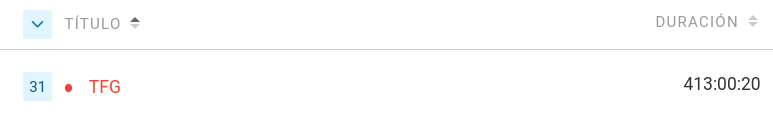
\includegraphics[scale=0.4]{doc/imagenes/clockfy.png}}
    \caption{Registro de horas trabajas en el proyecto en Clockify}
    \label{fig:clockify}
\end{figure}

\subsection{Costes de recursos materiales}
Una vez hemos calculado los costes de recursos humanos, es momento de calcular los costes de recursos materiales. Para su cálculo se deberá de tener en cuenta que los recursos sufren de un fenómeno llamado \textit{depreciación} el cual hace que estos sean devaluados con el paso del tiempo. \bigskip

Como se ha expuesto en la sección \ref{materiales} sólo se utilizará una sóla herramienta, el portátil personal de la estudiente. Para calcular su actual precio se aplicará el método de depreciación lineal usado para conocer la reducción del valor de un bien. 

\begin{table}[]
\begin{tabular}{|l|l|l|l|l|}
\hline
\rowcolor[HTML]{CCCCCC} 
\cellcolor[HTML]{CCCCCC}\textbf{Recurso} & \textbf{\begin{tabular}[c]{@{}l@{}}Valor\\ inicial(€)\end{tabular}} & \textbf{\begin{tabular}[c]{@{}l@{}}Valor\\ residual(€)\end{tabular}} & \textbf{\begin{tabular}[c]{@{}l@{}}Antigüedad\\ (años)\end{tabular}} & \textbf{\begin{tabular}[c]{@{}l@{}}Valor\\ actual\\ (€)\end{tabular}} \\ \hline
\rowcolor[HTML]{FFFFFF} 
\textbf{Portátil personal}& 899 & 179,8 & 4 & 323,64  \\ \hline
\rowcolor[HTML]{FFFFFF} 
\textbf{TOTAL} & & & & 323,64  \\ \hline
\end{tabular}
\caption{Tabla de los costes materiales}
\end{table}

Para calcular la depreciación se deberá antes calcular el valor residual del dispositivo el cual es el valor que poseerá al final de la vida útil del mismo. Suponemos para ello, que la vida útil de un portátil es de 5 años: 

\begin{equation}
    Valor\ residual = \frac{Coste\ inicial}{Vida\ util\ (a\tilde{n}os)} = \frac{899 \ \EUR}{5 \ a\tilde{n}os} = 179,8\ \EUR{}
\end{equation}

 Una vez conocido el valor residual, la depreciación se calcula de la siguiente forma:
\begin{equation}
    Depreciacion = \frac{Coste \ inicial - Valor\ residual}{Vida\ util\ ( a\tilde{n}os)} = \frac{899\EUR \ - \ 179,8\EUR }{5 \ a\tilde{n}os} = 143,84\ \EUR{}
\end{equation}

\subsection{Costes de recursos software, comunicación y documentación}
Los costes referentes a los recursos software son de 4.47€, debido a los costes ya explicados de la instancia de 0.47€ de AWS y 4€ por el dominio de Cloudfare. El resto del coste de los recursos software es nulo puesto que todos son de código abierto, a excepción de WebStorm que no es gratutito, puesto que se hace uso de la licencia gratuita para estudiantes de JetBrains. Por otro lado, en lo que respecta a los recursos utilizados para la documentación y comunicación son totalmente gratuitos salvo Visual Paradigm el cual es utilizado por una licencia gratuita ofrecida por la UGR.


\subsection{Costes adicionales}
Dentro de los costes adicionales se encuentran aquellos costes que no se han nombrado en los apartados anteriores, pero han sido necesarios para el desarrollo del proyecto. Estos costes son correspondientes a la factura de la luz e Internet:


\begin{table}[H]
\centering
\begin{tabular}{cc}
\hline
\multicolumn{1}{l}{\textbf{Recurso}} & \multicolumn{1}{l}{\textbf{Importe (€/mes)}} \\ \hline
Luz                                  & 25                                           \\
Internet                             & 70                                           \\ \hline
\end{tabular}
\caption{Tabla de los costes adicionales}
\end{table}

\subsection{Presupuesto total}
En la siguiente tabla se presenta la visión global de los costes de este proyecto:

\begin{table}[H]
\centering
\begin{tabular}{lc}
\hline
\textbf{Recurso}                                                                                      & \multicolumn{1}{l}{  \textbf{Importe}} \\ \hline
\textbf{Costes de recursos humanos}                                                                   & \multicolumn{1}{l}{}                 \\
Trabajo autónomo                                                                                      & 3997,84€                            \\ \hline
\textbf{Costes de recursos materiales}                                                                & \multicolumn{1}{l}{}                 \\
Portátil personal                                                                                     & 323,64€                              \\ \hline
\textbf{Costes de recursos software}                                                                  & \multicolumn{1}{l}{}                 \\
Elementary OS                                                                                         & 0,0€                                 \\
WebStorm                                                                                              & 0,0€                                 \\
Git                                                                                                   & 0,0€                                 \\
Github                                                                                                & 0,0€                                 \\
Docker                                                                                                & 0,0€                                 \\
Docker Compose                                                                                        & 0,0€                                 \\
Node.js                                                                                                & 0,0€                                 \\
Angular                                                                                               & 0,0€

\\
MongoDBAtlas                                                                                               & 0,0€

\\
Postman                                                                                               & 0,0€  

\\
AWS                                                                                               & 0,47€ 

\\
Cloudfare                                                                                               & 4,0€  

\\
Let's Encrypt                                                                                               & 0,0€  

\\ \hline
\textbf{\begin{tabular}[c]{@{}l@{}}Costes de recursos de\\ comunicación y documentación\end{tabular}} & \multicolumn{1}{l}{}                 \\
Draw.io                                                                                               & 0,0€   
             \\
Figma                                                                                                & 0,0€  
\\
Milanote                                                                                              & 0,0€                                 \\
Overleaf                                                                                              & 0,0€                                 \\
Visual Paradigm                                                                                       & 0,0€                                 \\
Google Meet                                                                                           & 0,0€                                 \\
Correo UGR                                                                                            & 0,0€                                 \\
Clockify                                                                                                & 0,0€                                 \\ \hline
\textbf{Costes adicionales}                                                                           & \multicolumn{1}{l}{}                 \\
Factura de la luz                                                                                     & 25€ x 3 meses = 75€                                 \\
Factura de Internet                                                                                   & 70€  x 3 meses = 225€                                \\ \hline
\textbf{TOTAL}                                                                                        & \multicolumn{1}{l}{4.625,95€}       
\end{tabular}
\caption{Tabla del presupuesto total del proyecto}
\end{table}

\section{Gestión de riesgos} \label{riesgos}
Durante el desarrollo de todo proyecto se tiene siempre la posibilidad de que puedan manifestarse ciertas situaciones que supongan un obstáculo o incluso amenaza para su correcta evolución. Es por ello que por mínima que sea la posibilidad de que ocurran hay que estar preparado y para ello se debe de precisar un plan de actuación.

En esta sección se identificarán los posibles riesgos a correr durante el proyecto, sus causas y el plan de actuación en caso de ser materializados para solventar o reducir lo máximo posible su impacto. Posteriormente se hará una estimación de la probabilidad de aparición y del impacto que supone cada uno de ellos.

\subsection{Identificación de riesgos}
Los posibles riesgos para el desarrollo del proyecto identificados son mostrados en la siguiente tabla (Figura \ref{fig:riesgos}):

\begin{figure}[H]
    \centering{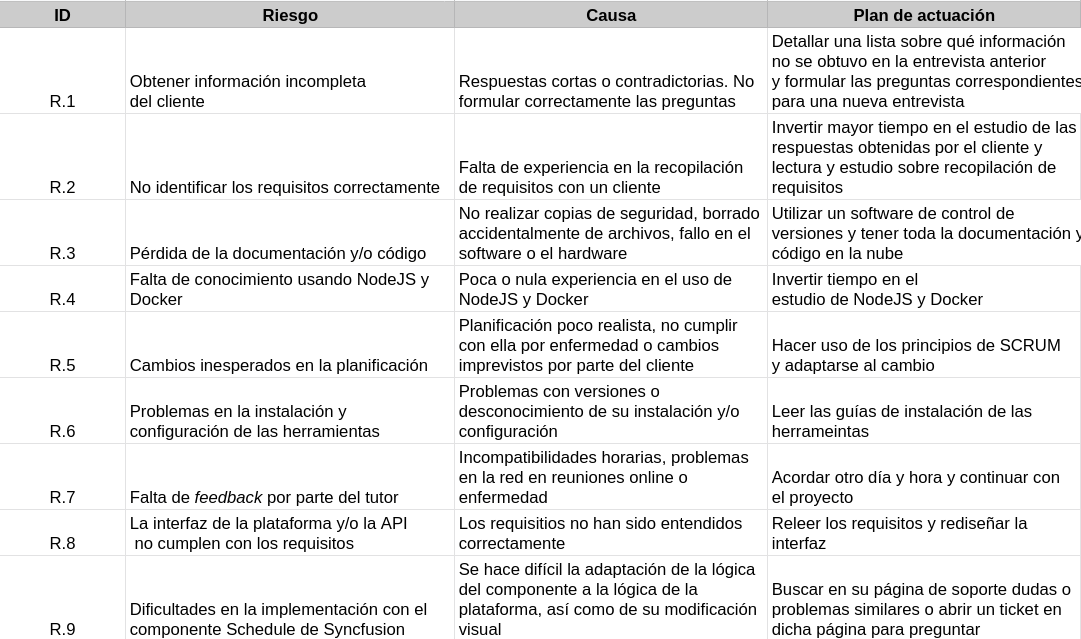
\includegraphics[scale=0.35]{doc/imagenes/riesgos.png}}
    \caption{Tabla de riesgos del proyecto}
    \label{fig:riesgos}
\end{figure}
\subsection{Análisis de riesgos}
Para analizar los riesgos expuestos anteriormente, se ha hecho uso de una matriz de probabilidad-impacto:

\begin{figure}[H]
    \centering{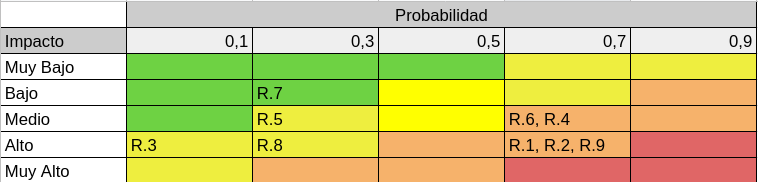
\includegraphics[scale=0.4]{doc/imagenes/analisis-riesgos.png}}
    \caption{Matriz de probabilidad-impacto de riesgos}
    \label{fig:analisis-riesgos}
\end{figure}

\subsection{Riesgos materializados} \label{riesgos-materializados}
Los riesgos surgidos durante el transcurro del desarrollo del proyecto han sido precisamanete los marcados con mayor probabilidad en la matriz de probabilidad-impacto \ref{fig:analisis-riesgos} (R.1, R.2, R.4 y R.6) . La falta de experiencia ante el reto que supone recoger información de un cliente ha provocado que surgieran numerosas dudas acerca de los requisitos del proyecto. A su vez la utilización de Docker y Node.js por primera vez ha evocado a invertir gran parte del tiempo del primer sprint en su instalación y estudio. Por último, el riesgo R.9 ha sido materializado, el cual ha resultado ser bastante crítico durante la realización del proyecto. Esto se debe a que supuso la alteración de la planificación debido a la caótica y escasa documentación presentada por Syncfusion para el componente del calendario y las largas esperas en su plataforma de soporte ante dudas planteadas. \bigskip

A pesar de la manifestación de los riesgos nombrados se ha sabido aplicar correctamente el plan de actuación previamente establecido para cada uno.

    % Diseño
	\chapter{Diseño} \label{disenio}
En este cuarto capítulo se establecerá la estructura de la plataforma, no sólo a nivel técnico, sino también a nivel visual. Primeramente se definirá la arquitectura que presentará la plataforma, explicando cada uno de los elementos que la conforman, base de datos, servidor y cliente. Para ello, tanto en el servidor, como en el cliente se expondrán dos diagramas UML de paquetes diseñados siguiendo las indicaciones del artículo \textit{''An Overview of Structural
UML Diagrams''}\cite{bhatt2021overview}.

\section{Arquitectura MEAN}
\begin{figure}[H]
    \centering{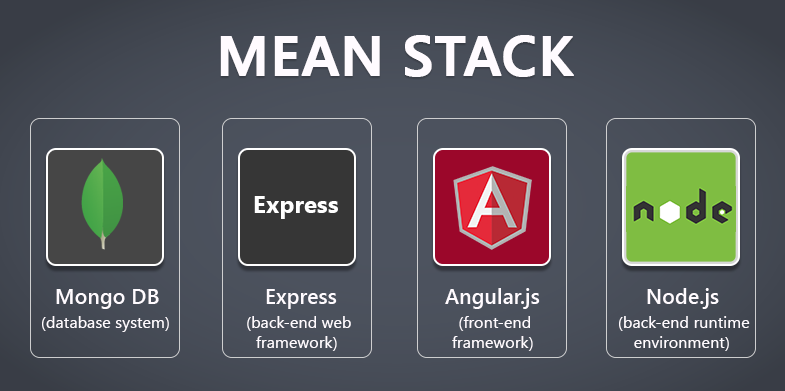
\includegraphics[scale=0.4]{doc/imagenes/mean.png}}
    \caption{Stack MEAN (Mongo, Express, Angular y Node)}
    \label{mean}
\end{figure}

Para la arquitectura del proyecto se ha optado por hacer uso del stack software MEAN \cite{nirgudkar2017mean} (Figura \ref{mean}), acrónimo que hace referencia a las tecnologías que lo conforman: MongoDB, Express.js, Angular y Node.js. 

\begin{figure}[H]
    \centering{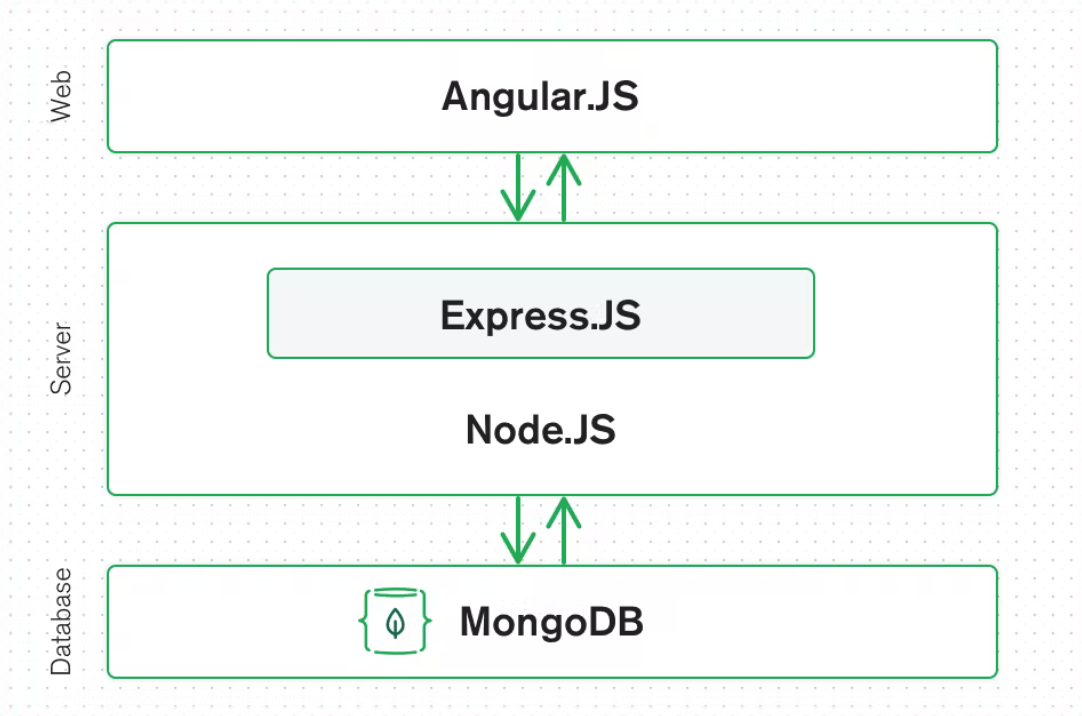
\includegraphics[scale=0.25]{doc/imagenes/mean-architecture.png}}
    \caption{Arquitectura en capas de MEAN}
    \label{mean-architecture}
\end{figure}

Se trata de un stack software basado en JavaScript para el desarrollo de aplicaciones web, cuyo diseño hace una división en capas de la parte del cliente, el servidor y la base de datos (Figura \ref{mean-architecture}). \bigskip

Se ha decidido aplicar este stack en concreto a la arquitectura del proyecto por varios motivos. El primero es que, a pesar de que la desarrolladora no había trabajado anteriormente con las tecnologías Express.js y Node.js, sí que lo había hecho con Angular y MongoDB, por lo que esa falta de experiencia en el desarrollo de la parte del servidor es compensada. Otro de los motivos a mencionar es que MEAN es de código abierto, y en consecuencia no sólo abarata el coste del proyecto, sino que también significa que la documentación de la que se dispone sea considerablemente extensa debido su gran comunidad de soporte. Por supuesto, un punto muy positivo que presenta MEAN, tal y como afirma Bakwa D. Dunka et al. \cite{dunka2018simplifying}, es el uso de JavaScript en la capa del servidor y del cliente, lo cual conlleva mayor simplicidad en la implementación y no se necesita aprender un nuevo lenguaje. Asimismo, otra característica realmente positiva a mencionar es la complicidad que existe entre sus tecnologías, pues, como se comentará más adelante, en la parte del cliente se va a utilizar el componente Angular Schedule de Syncfusion \footnote{\url{https://ej2.syncfusion.com/angular/documentation/schedule/getting-started/}}, el cual se trata de un componente de Angular que trabaja con datos de tipo JSON para las citas. En cuanto al uso de la base de datos no relacional con MongoDB, resulta perfecto ya que las citas vendrán acompañadas de descripciones potencialmente largas y sin formato. Por último, resaltar una característica mencionada en el artículo escrito por Sanchit Aggarwal et al. \cite{aggarwal2018comparative}: el buen rendimiento presentado por Angular para manejar un gran número de datos, ya que en cuanto a lo que concierne a este proyecto un calendario en cierto momento llegará a contener cientos de citas.

\subsection{Diseño de la base de datos} \label{bd}

Para el diseño de la base de datos se han planteado las siguientes dos colecciones (Figura \ref{bd}):

\begin{figure}[H]
    \centering{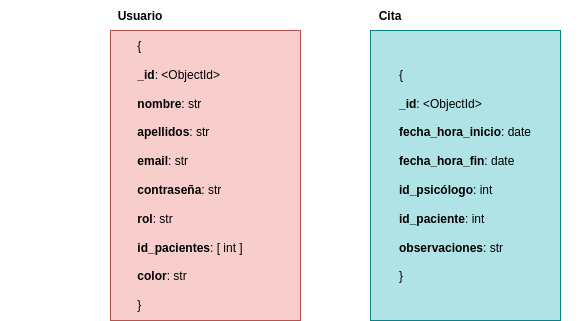
\includegraphics[scale=0.5]{doc/imagenes/bd.png}}
    \caption{Diagrama de la base de datos}
    \label{bd}
\end{figure}

La base de datos consta de dos colecciones: \textbf{Usuario} y \textbf{Cita}. La primera contiene el id del usuario, nombre, apellido, email, contraseña encriptada y rol del éste en la plataforma (administrador, paciente o psicólogo). Además de estos campos el rol de psicólogo posee un array de ids de pacientes y un color asignado para las citas, si no se poseyera este rol ambos campos serian nulos en el documento. Por otro lado, la colección de Cita contiene el id de la cita, la fecha y hora de inicio y fin de ésta, un campo para posibles observaciones y los ids del paciente y psicólogo de este.

\subsection{Diseño del servidor}

\subsubsection*{Diagrama de paquetes }
En el diseño del servidor de Node.js Express, se ha divido su funcionamiento en 3 componentes (Figura \ref{fig:paquetes-back}) para modularizar y desacoplar funcionalidades: los controladores, los modelos y las rutas. Los controladores serán los encargados de manejar toda la lógica de la aplicación, los modelos represetarán las estructuras de datos de la plataforma y las rutas contendrán los endpoints a los que los usuarios accederan para hacer peticiones a los controladores:

\begin{figure}[H]
    \centering{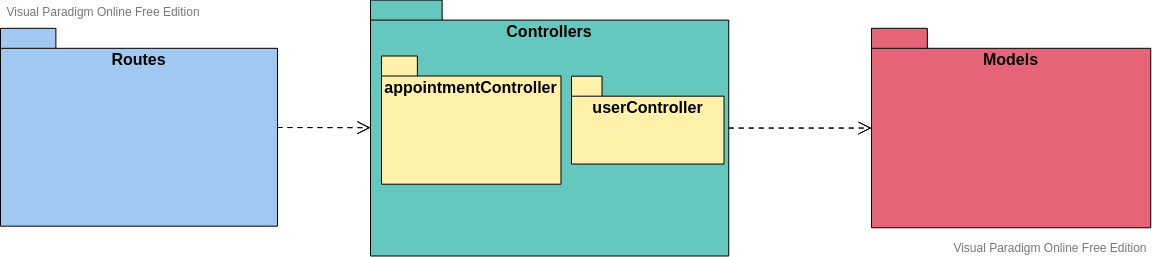
\includegraphics[scale=0.2]{doc/imagenes/package-back.png}}
    \caption{Diagrama de paquetes del backend}
    \label{fig:paquetes-back}
\end{figure}

\subsection{Diseño del cliente}

\subsubsection*{Diagrama de paquetes}
Para el diseño del cliente se ha planteado el siguiente diagrama de paquetes (Figura \ref{fig:paquetes-frontend}) en el que se expone la agrupación de cada componente de Angular en el frontend, donde el componente protagonista es el componente ''main'', el cual en función de la ruta en la que se encuentre el usuario cambiará el componente mostrado.:

\begin{figure}[H]
    \centering{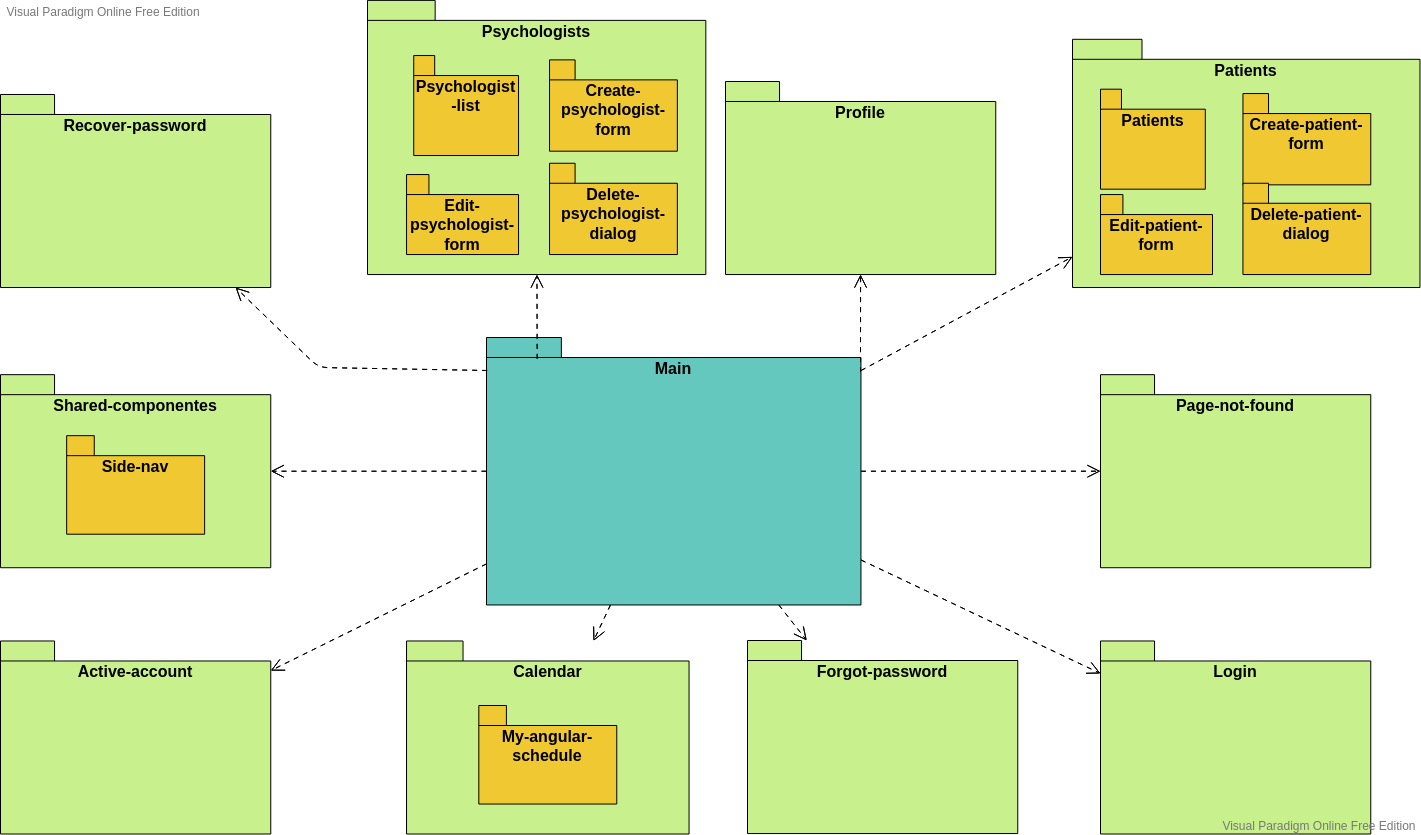
\includegraphics[scale=0.2]{doc/imagenes/diagrama-paquetes-front.png}}
    \caption{Diagrama de paquetes del frontend}
    \label{fig:paquetes-frontend}
\end{figure}

\subsubsection*{Usabilidad y Accesibilidad}
En el diseño de la interfaz de la plataforma se hará uso de Angular Material, siguiendo las guías de diseño proporcionadas por Google Material \footnote{\url{https://material.io/design/guidelines-overview}} para conseguir un diseño, no sólo visualmente estético, sino también usable y accesible proporcionando una experiencia de usuario personalizada. Así lo manifiesta en su libro Venkata Keerti Kotaru \cite{kotaru2020material}, pues la combinación de dicha librería junto con Angular y Typescript generan una poderosa combinación para generar atrativas interfaces de usuario\bigskip

Para el diseño de la interfaz de la plataforma se pretende poner al usuario ante todo, estructurando una web sencilla e intuitiva y evitando todos los puntos negativos comentados en el Capítulo \ref{estado-arte} del Estado del Arte donde se encontraban plataformas con flujos de usuario complejos, poco funcionales. Para ello se ha consultado el libro \textit{''Design Principles in the Development of Dashboards for Business Management''} \cite{martins2022design}. Además, se pretende obtener una interfaz responsiva tanto para tablets como para móviles, siguiendo los consejos de diseño para este tipo de interfaces de Wenjie Li et al. \cite{li2022design}.  \bigskip

Primeramente se debe de definir a qué usuarios se dirige la web. En este caso, los perfiles de usuario a abarcar son numerosos, pues por un lado el personal de la clínica está compuesto por personas con un rango de edad entre 29 y 54 años con conocimientos básicos en la informática y por otro lado el rango de edad de los pacientes es mucho más extenso comprendiéndose, desde jóvenes adolescentes hasta ancianos, por lo que perfectamente habrá casos en los que los conocimientos en informática sean prácticamente nulos. Es por ello que el flujo de usuario debe de ser el más sencillo y directo posible. Siguiendo esta premisa, a continuación se han diseñado los sitemaps que seguirá la plataforma para usuarios identificados y no identificados (Figuras \ref{sitemap-no-identificado} y \ref{sitemap-identificado}), cuyo diseño cumple con las guías que ofrece Google Material para navegación \footnote{\url{https://material.io/design/navigation/understanding-navigation.html}} donde se distinguen tres tipos: navegación hacia adelante, reversa y lateral.

\begin{figure}[H]
    \centering{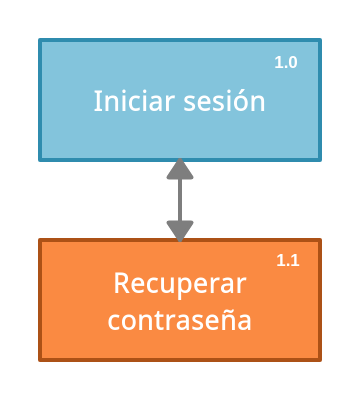
\includegraphics[scale=0.15]{doc/imagenes/sitemap-user-no-registered.png}}
    \caption{Sitemap para un usuario no identificado}
    \label{sitemap-no-identificado}
\end{figure}

\begin{figure}[H]
    \centering{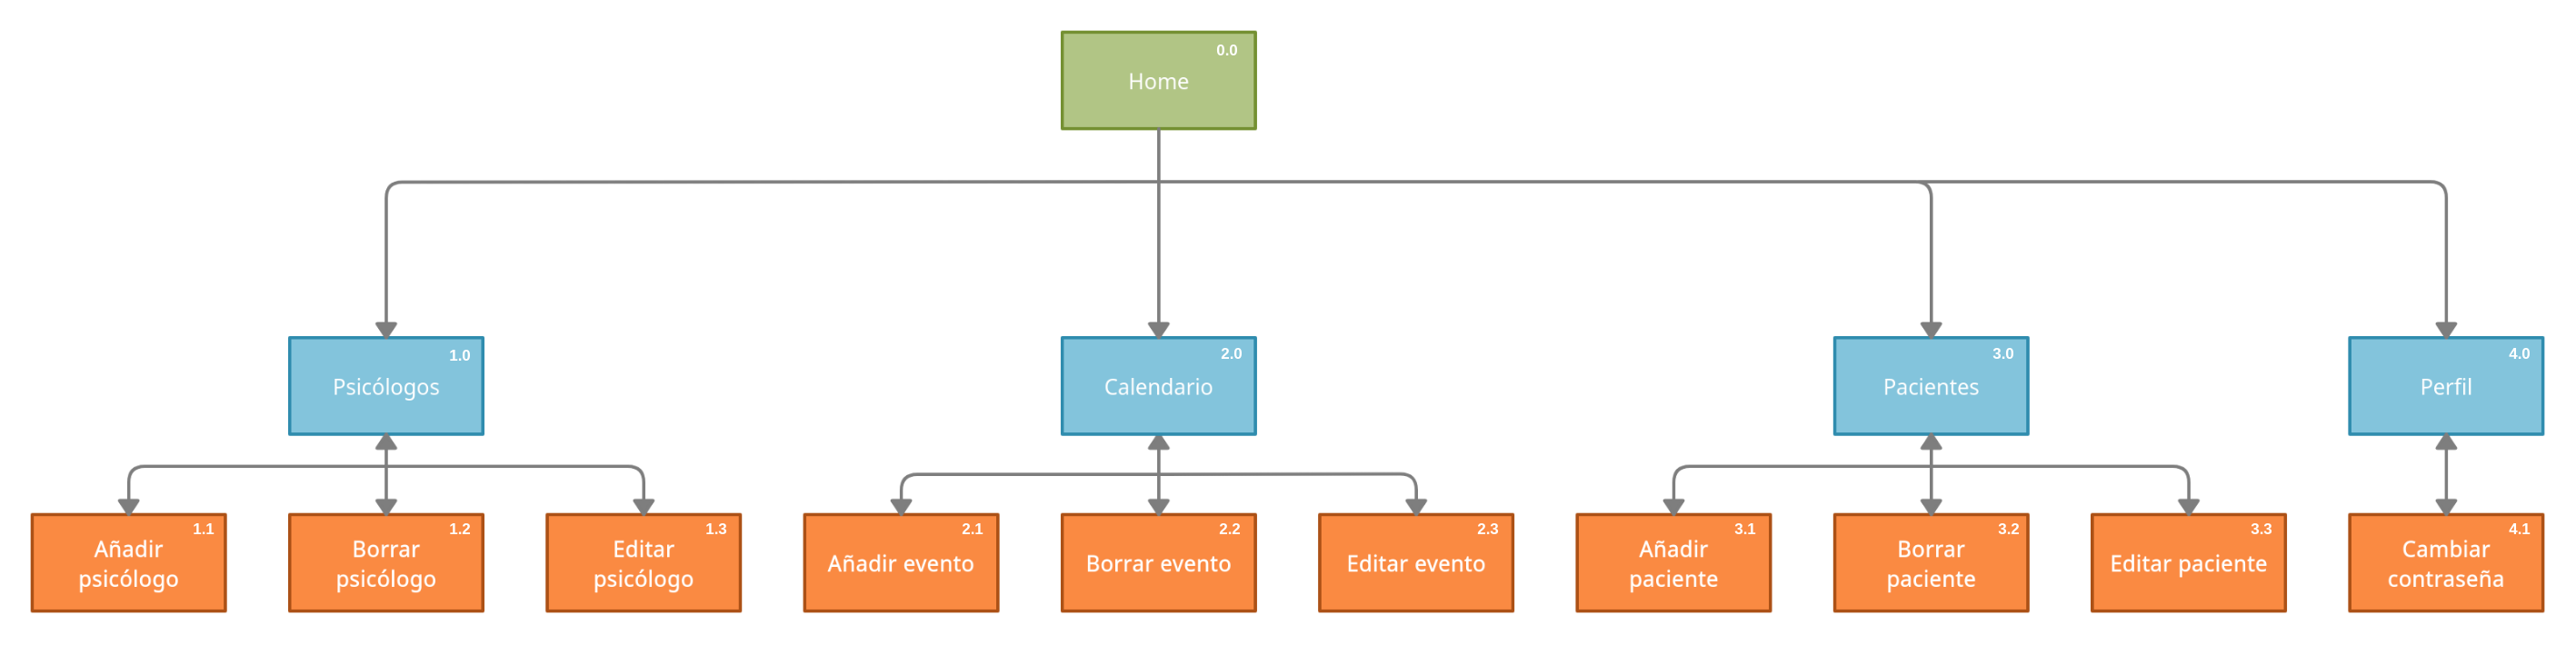
\includegraphics[scale=0.15]{doc/imagenes/sitemap-user-registrado.png}}
    \caption{Sitemap para un usuario identificado}
    \label{sitemap-identificado}
\end{figure}

Ahora que se ha definido la estructura de la página se puede definir el flujo que seguirán sus usuarios. En la definición de dichos flujos se ha pretendido que el usuario no encuentre dificultad alguna en la interacción con la plataforma. Para ello, el flujo seguido para las operaciones CRUD de citas, psicólogos y pacientes es, en esencia, el mismo (Figuras \ref{flow-calendario}, \ref{flow-pacientes} y \ref{flow-psicologos}). La diferencia es la entidad con la que se esta trabajando y el campo ''color'' de los psicólogos que no tienen los pacientes y el campo ''psicólogo'' que no tienen los psicólogos.

\begin{figure}[H]
    \centering{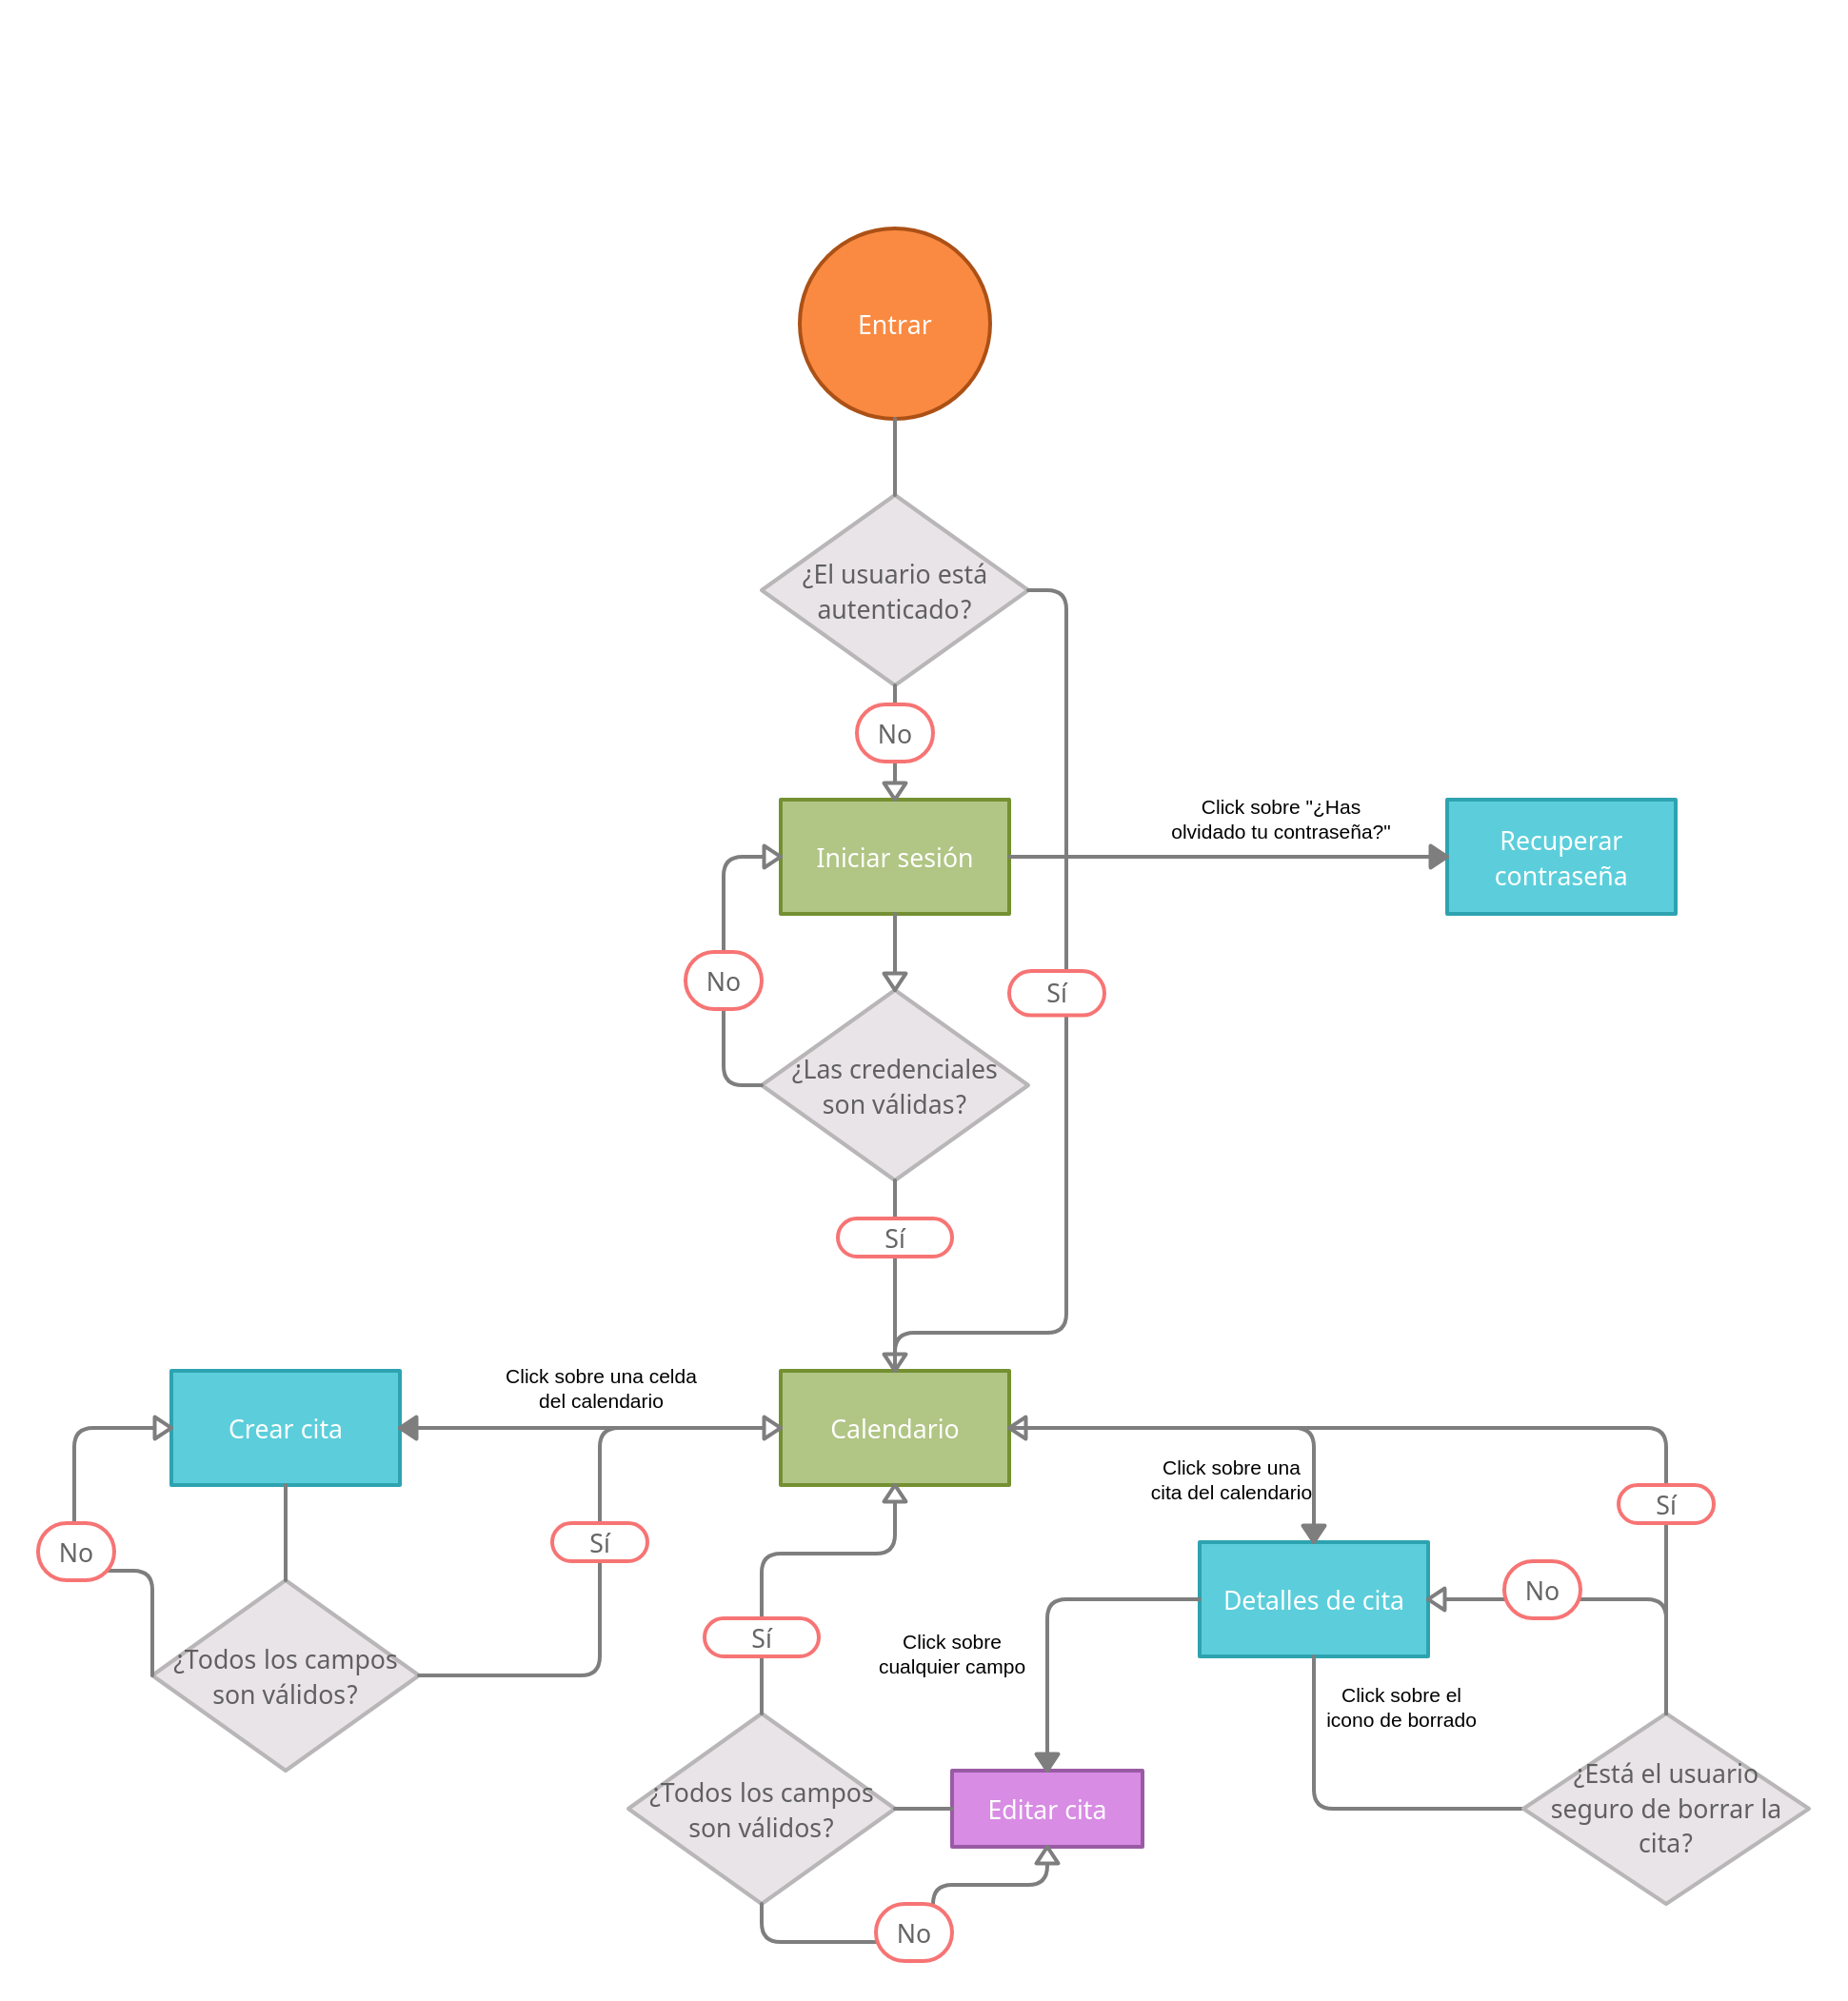
\includegraphics[scale=0.1]{doc/imagenes/flow-calendario.png}}
    \caption{Flujo de usuario para la sección de Calendario}
    \label{flow-calendario}
\end{figure}

\begin{figure}[H]
    \centering{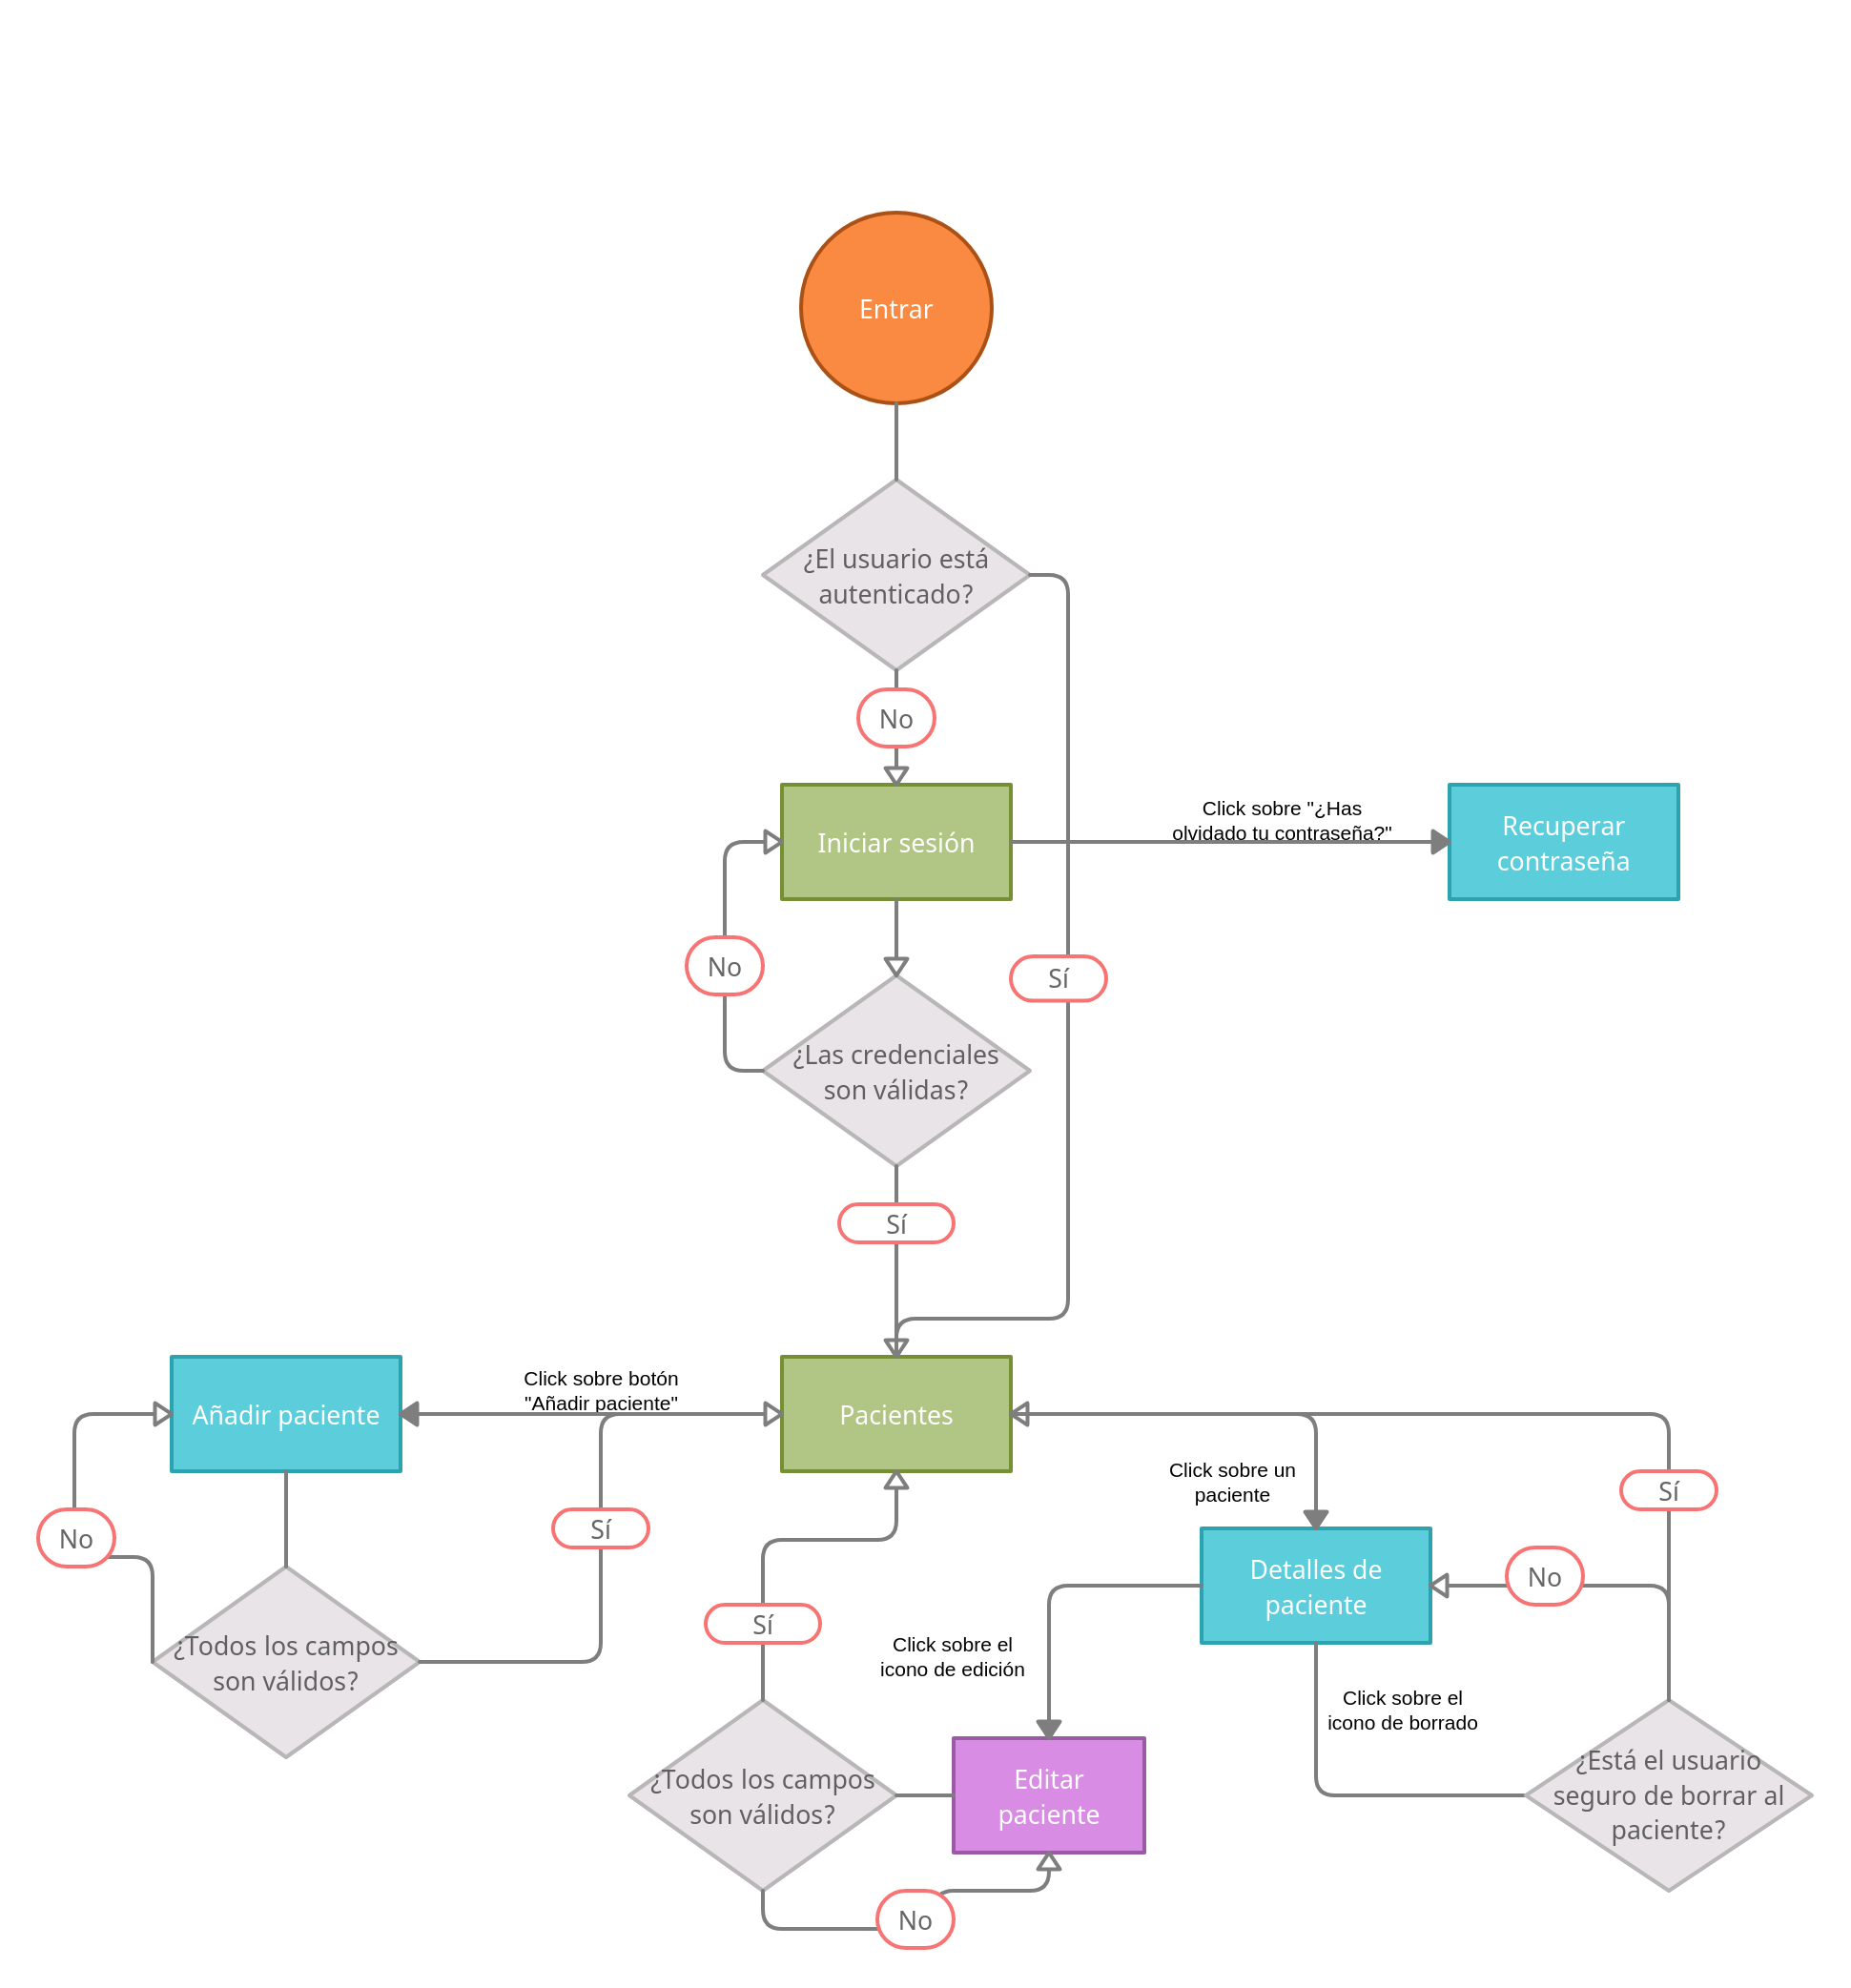
\includegraphics[scale=0.1]{doc/imagenes/flow-pacientes.png}}
    \caption{Flujo de usuario para la sección de Pacientes}
    \label{flow-pacientes}
\end{figure}

\begin{figure}[H]
    \centering{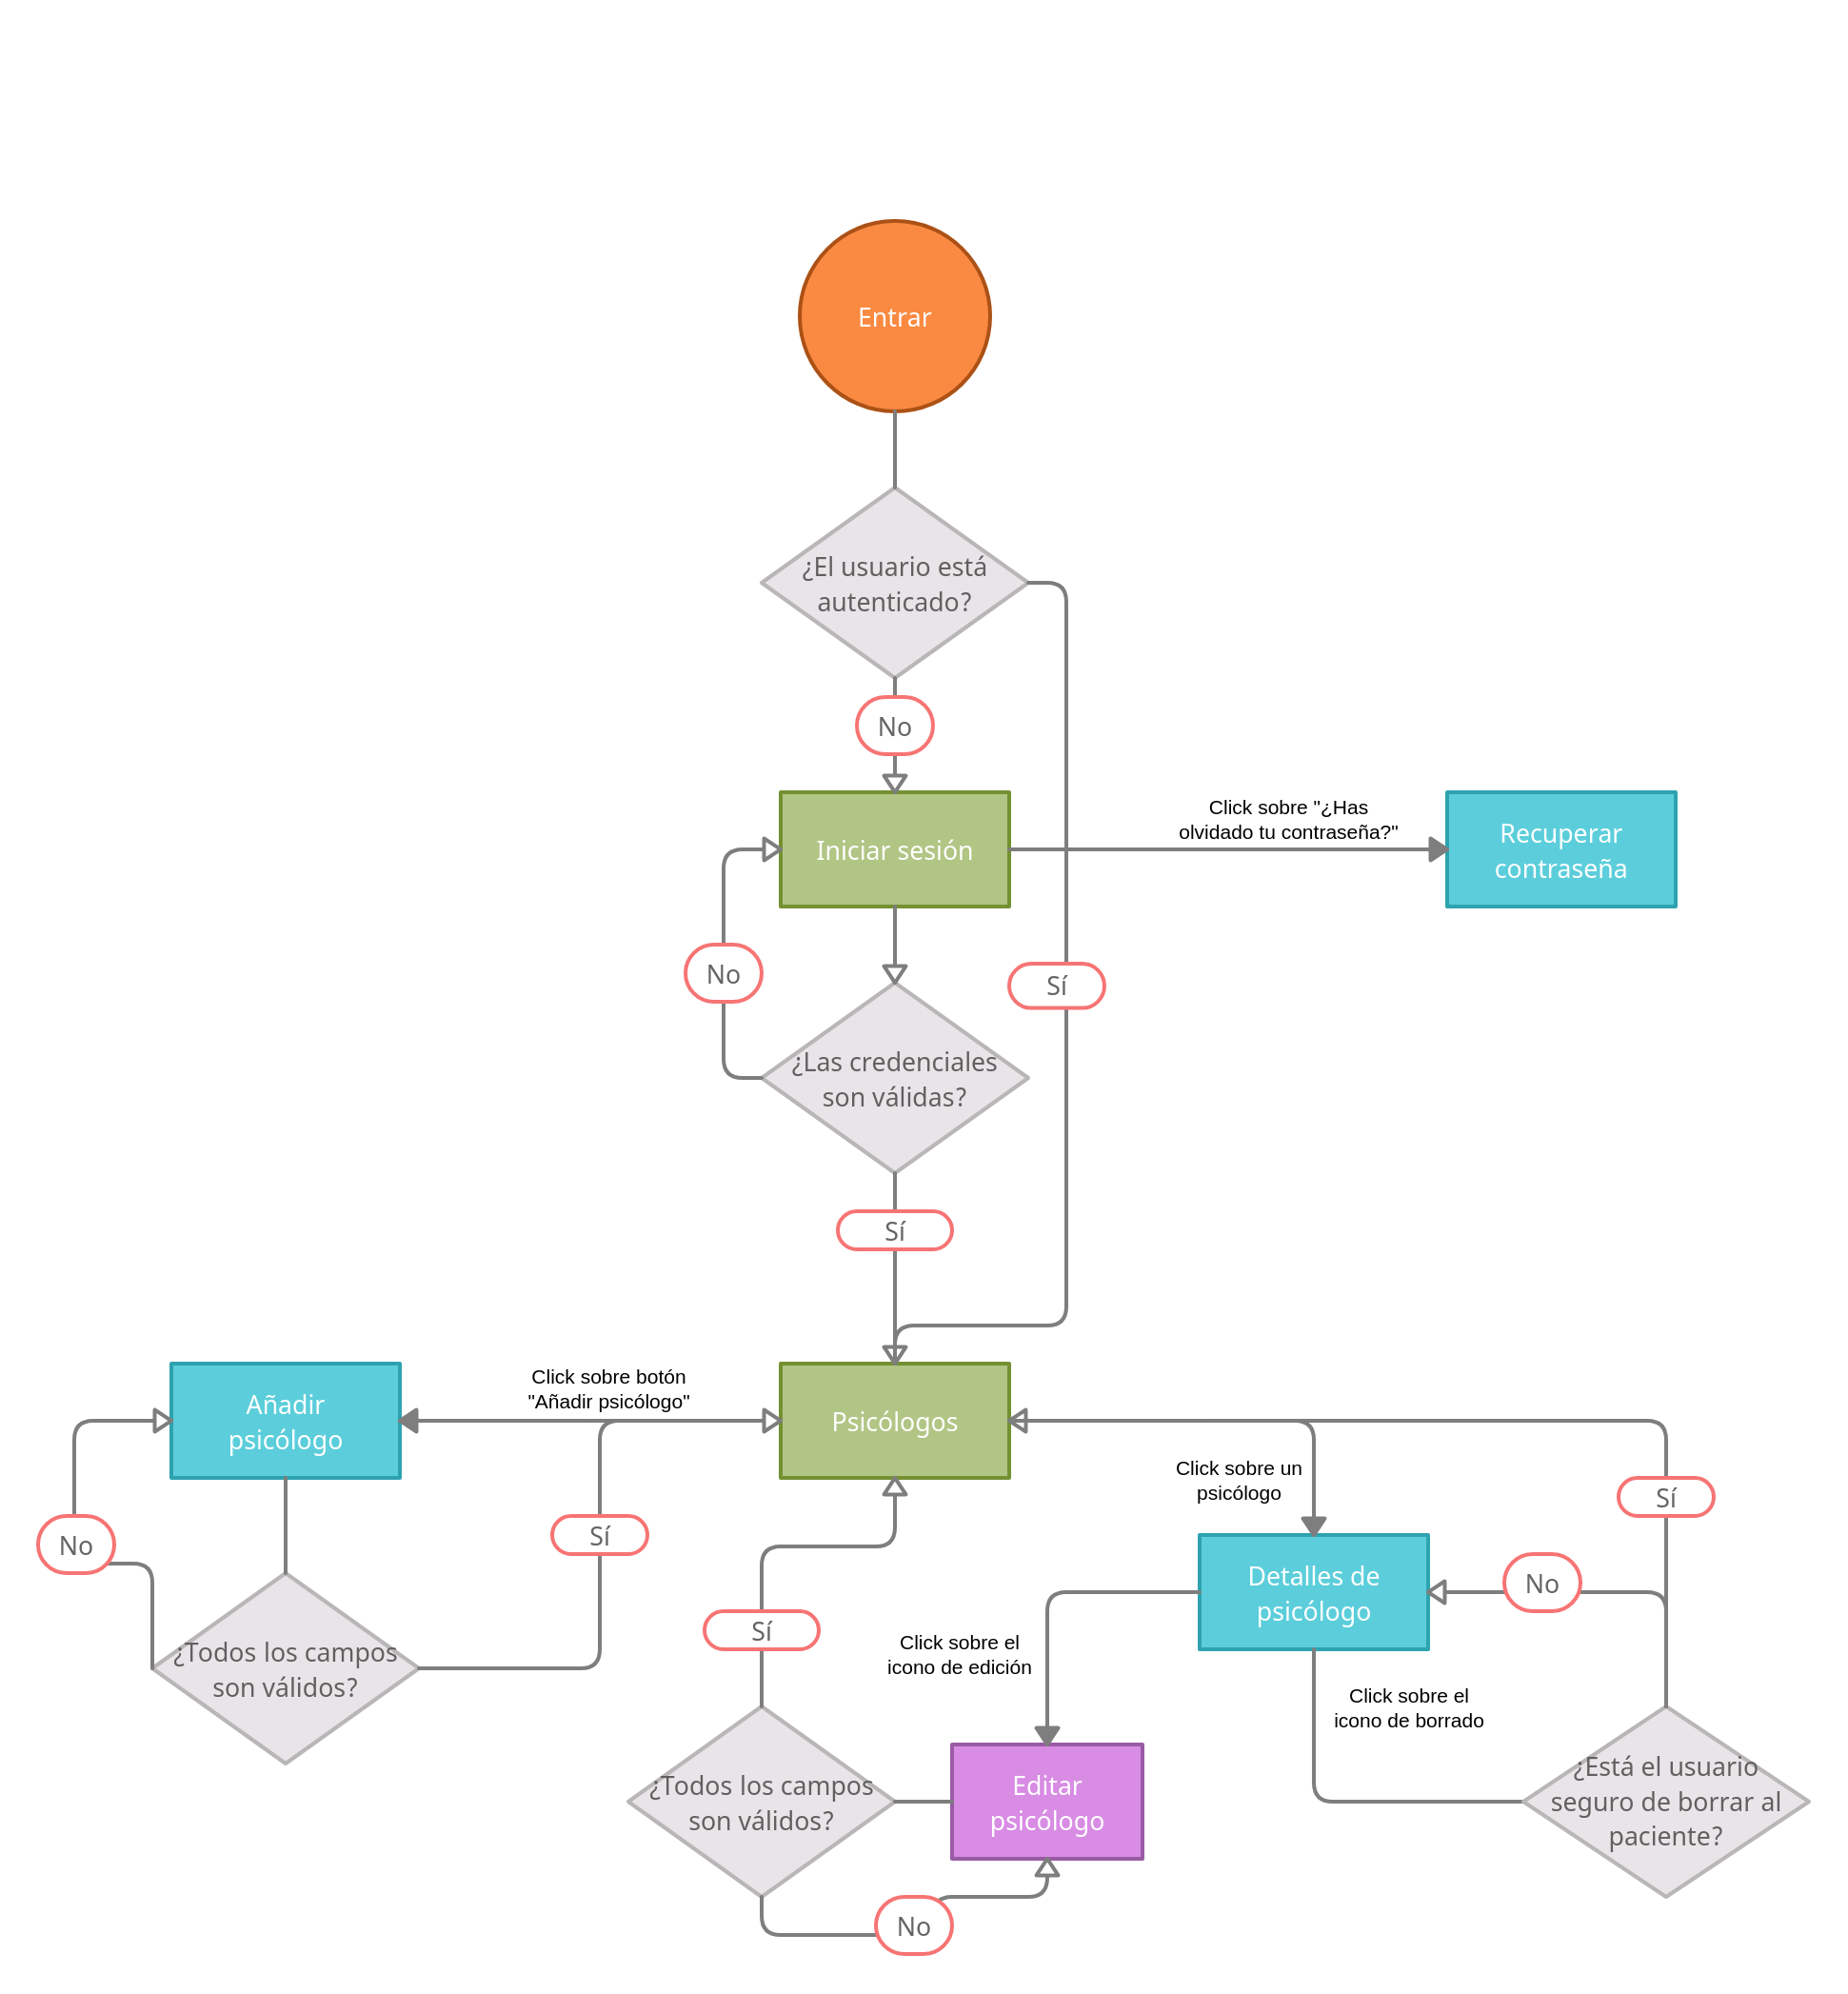
\includegraphics[scale=0.1]{doc/imagenes/flow-psicologos.png}}
    \caption{Flujo de usuario para la sección de Psicólogos}
    \label{flow-psicologos}
\end{figure}

Finalmente a estos flujos de usuario se añade el flujo de usuario de la sección de Perfil (Figura \ref{flow-perfil}).

\begin{figure}[H]
    \centering{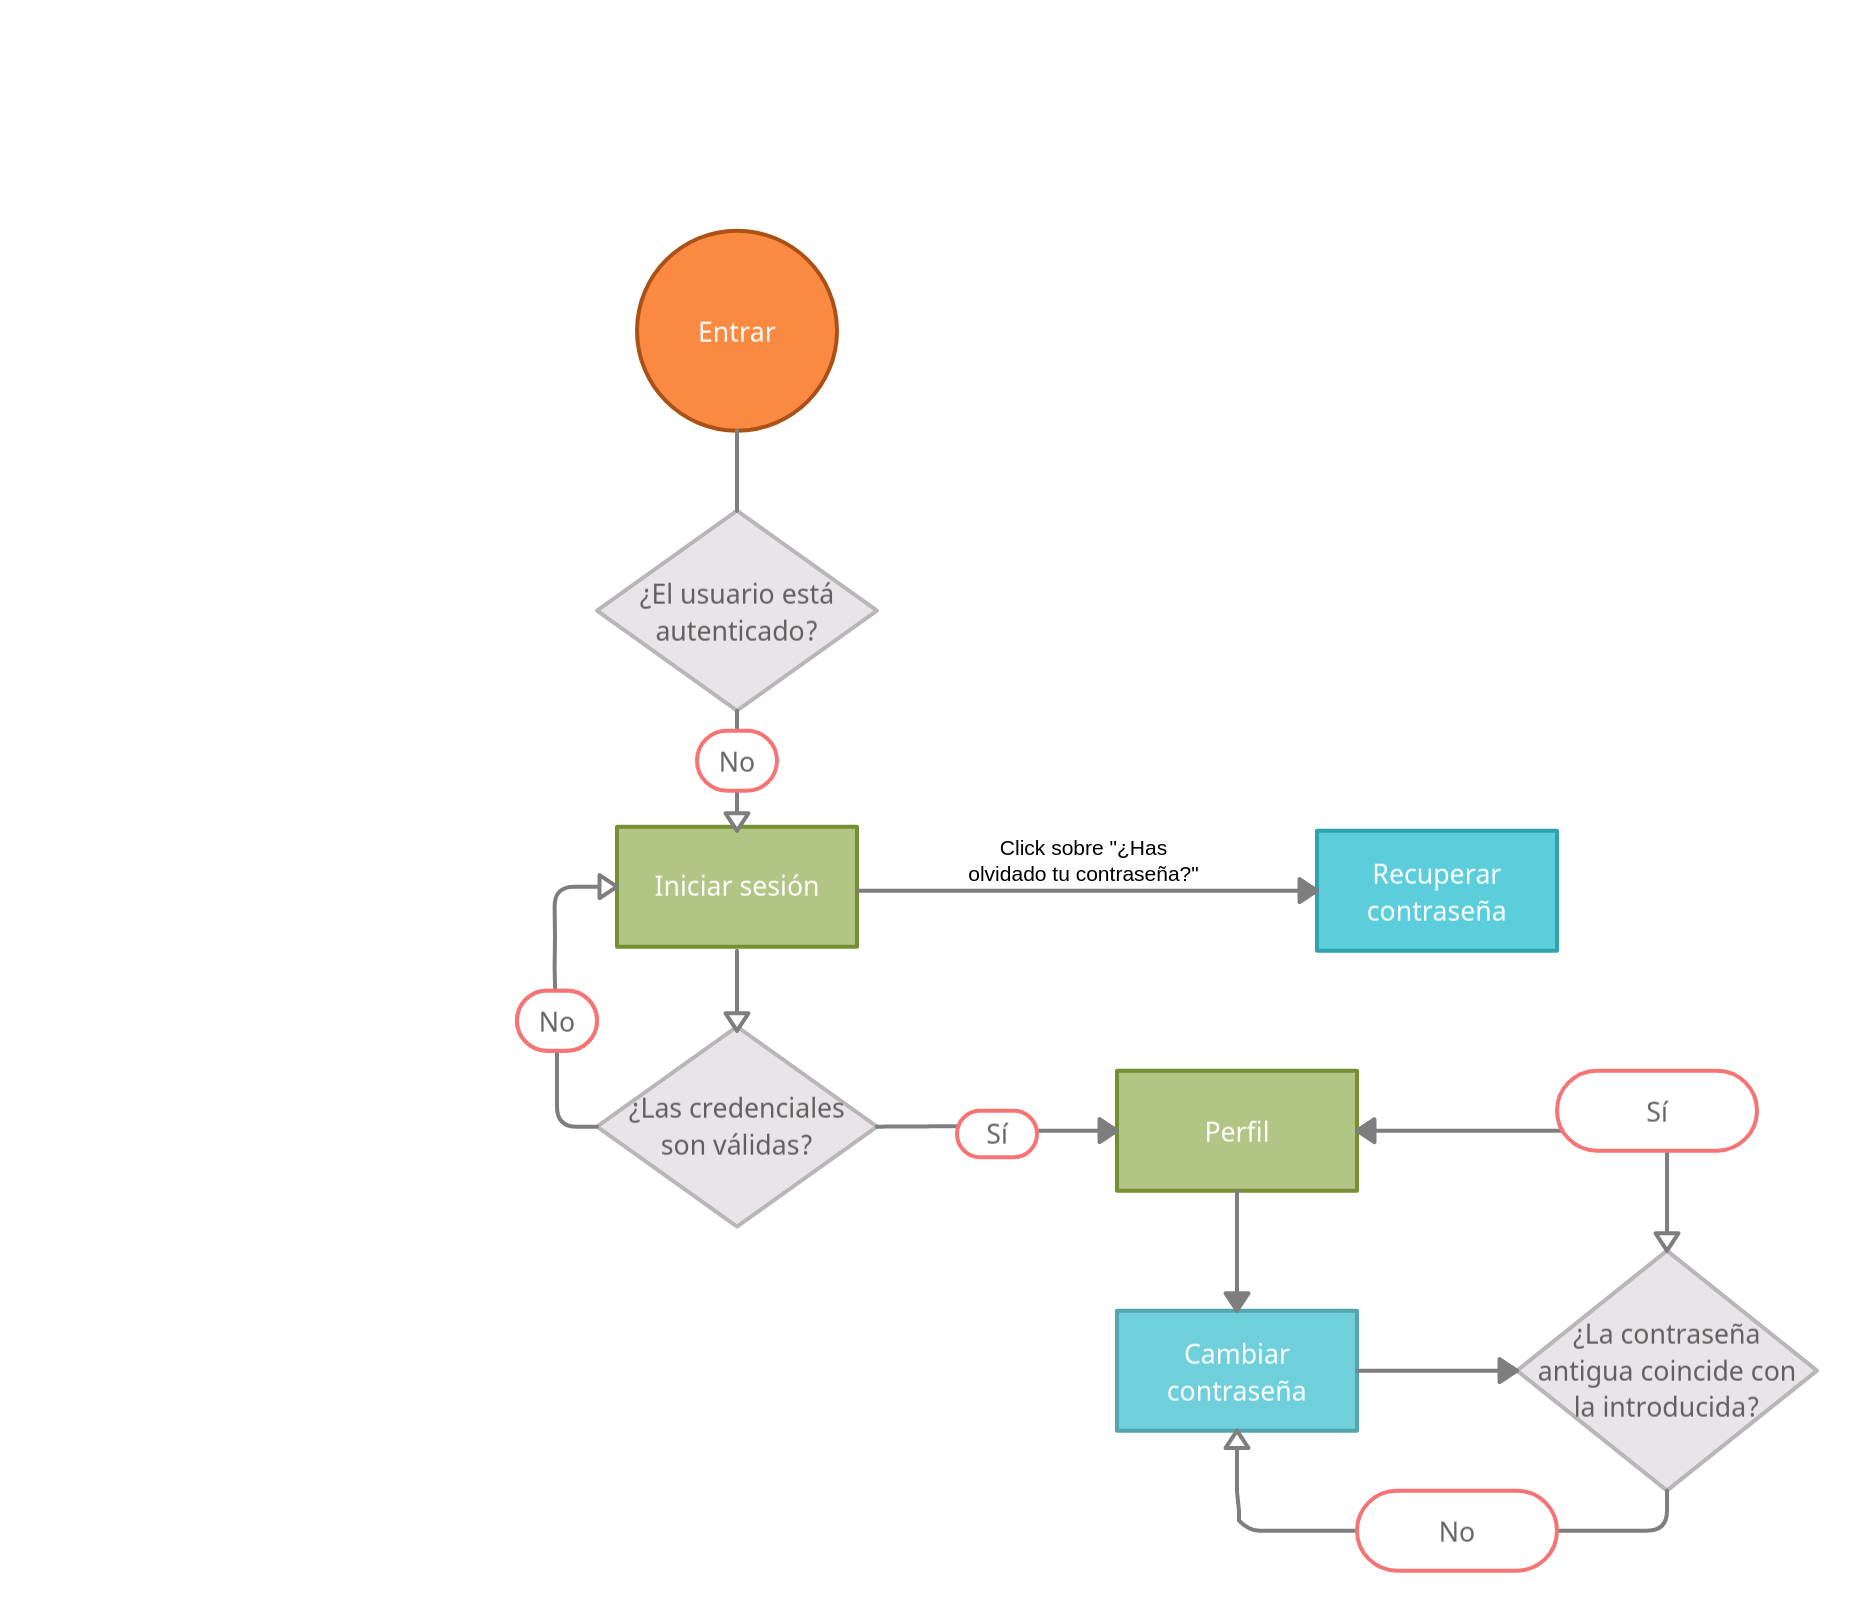
\includegraphics[scale=0.1]{doc/imagenes/flow-perfil.png}}
    \caption{Flujo de usuario para la sección de Perfil}
    \label{flow-perfil}
\end{figure}


Una vez ha sido definido el flujo de usuario en la plataforma, es momento de la parte más creativa del diseño en la que se definirá la actitud que se pretende transmitir a los usuarios y con ello se escogerá un nombre para la web, una paleta de colores, la elección de una fuente apropiada, un eslogan y la creación de un logo. \bigskip

Para establecer el tono y voz utilizado en la web se ha de tener en cuenta el contexto en el que se encuentra, el cual es el de un centro sanitario. Por tanto, el contenido que se va a ofrecer a los usuarios debe de ser profesional y serio. En consecuencia, la plataforma será lo más directa posible mostrando de forma clara las acciones a realizar en ella, así como los errores que se puedan dar. A su vez, se buscará transmitir una actitud calmada evitando el uso de palabras en mayúsculas o signos de exclamación. Ahora bien, a pesar de este tono profesional naturalmente no se ha de olvidar la cercanía que en todo momento se procura tener con los pacientes en el ámbito de la salud.\bigskip

Teniendo claro lo anterior, es hora de elegir un nombre para la plataforma. Para su elección se han tenido numerosas ideas combinando los conceptos de tiempo y cita médica como ''HTime'', ''Mediatrics'', ''HeyPlannect'',''iAppointment'', ''Dation'', etc. Sin embargo, finalmente la opción elegida ha sido \textbf{''DayDay''} por su sencillez y facilidad para recordar. De igual forma para el eslogan se barajaron múltiples opciones, pero finalmente se escogió ''365 días en una página'' por las mismas razones. \bigskip

En cuanto a la elección de la paleta de colores, teniendo presente la actitud a transmitir a los usuarios que se ha definido anteriormente, se va a seguir para su elección el artículo escrito por Jicheng Yang y Xiaoying Shen ''The Application of Color Psychology in Community Health
Environment Design'' \cite{Yang2022} en el que se exponen los resultados obtenidos a través de una investigación llevada a cabo sobre la psicología del color en el ámbito de la salud. Yang y Shen afirman que cada color tiene su propia personalidad. Seguidamente se muestra en la Figura \ref{psicologia-color} los rasgos que representan a cada color:

\begin{figure}[H]
    \centering{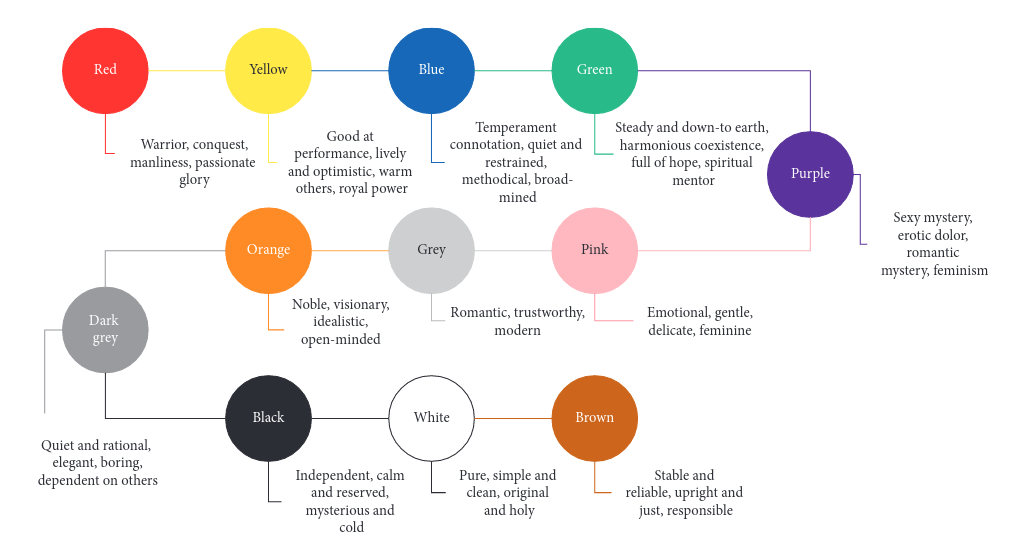
\includegraphics[scale=0.4]{doc/imagenes/psicologia-color.png}}
    \caption{Rasgos de personalidad del color \cite{Yang2022}}
    \label{psicologia-color}
\end{figure}

A través de dicha figura se observan ciertos rasgos con los que DayDay se identifica: la sencillez y pureza del blanco, la harmonía del verde, la paz del azul, la fiabilidad del marrón, la confianza del gris o la nobleza del naranja. Tomando en consideración esto y buscando un diseño lo más accesible posible, se ha elegido la siguiente paleta (Figura \ref{paleta}) por sus contrastres:

\begin{figure}[H]
    \centering{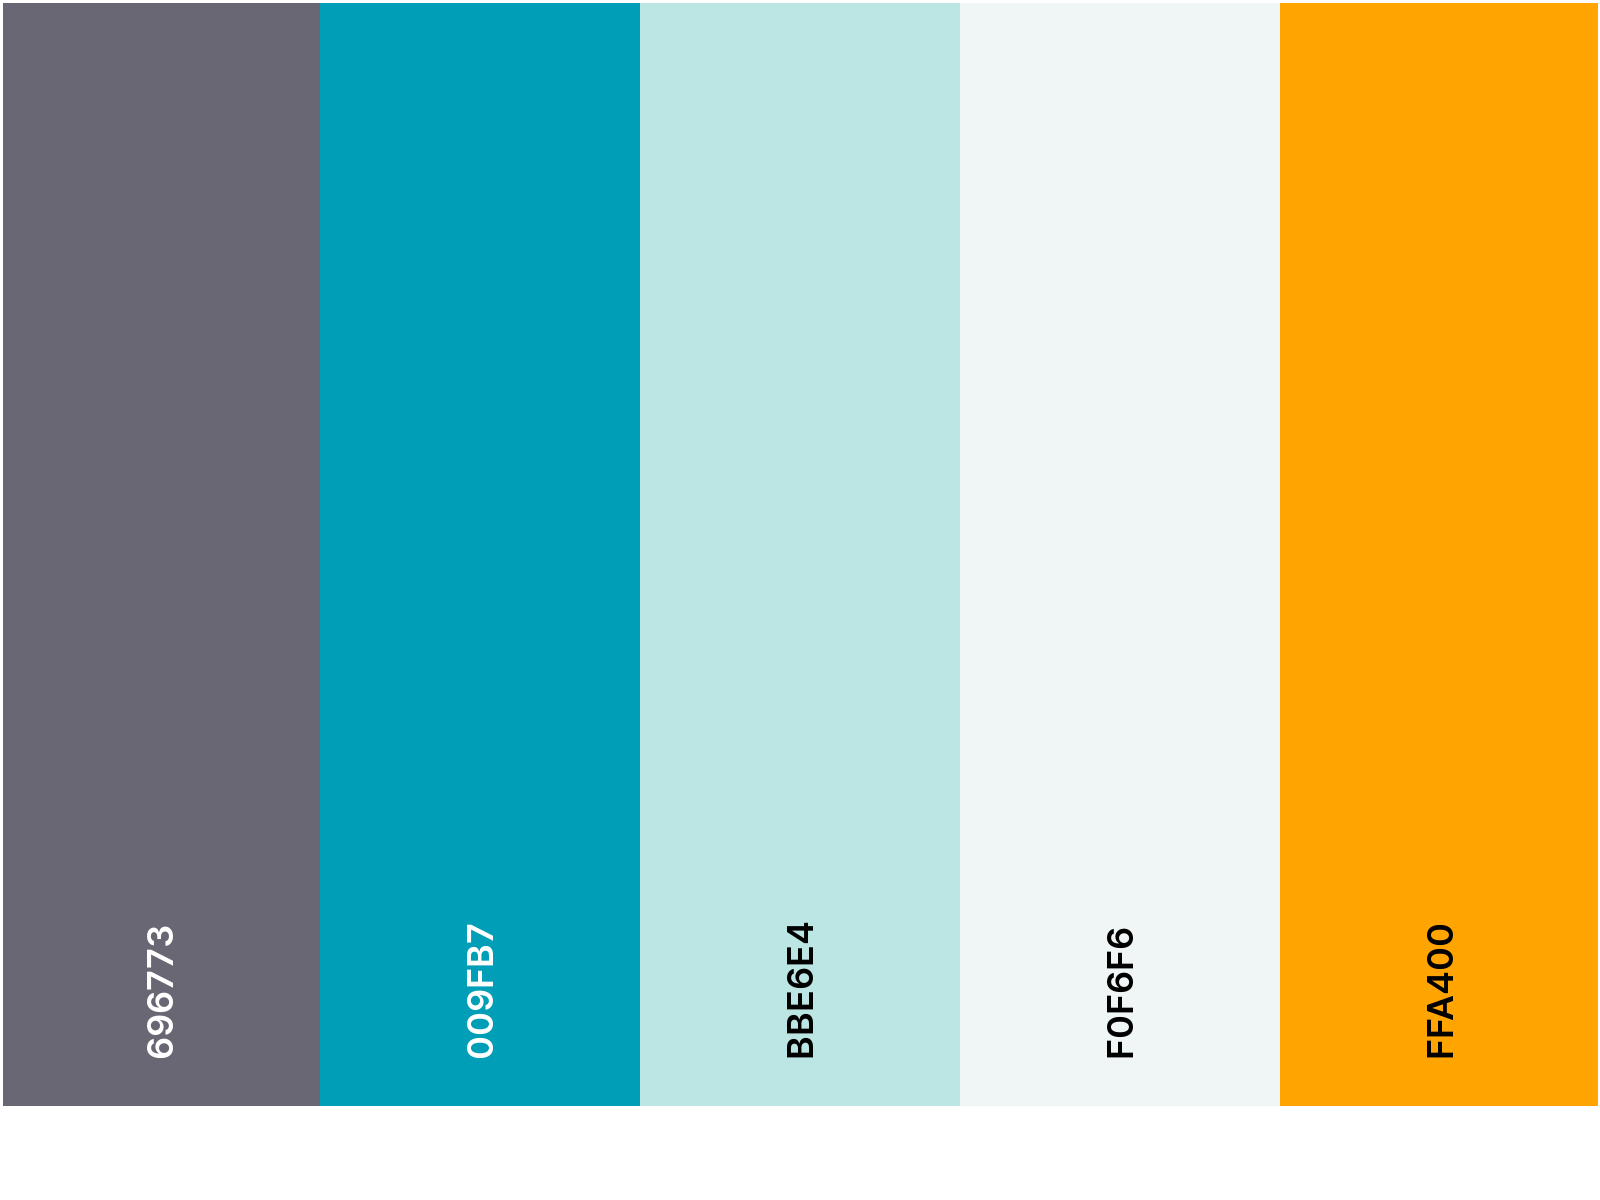
\includegraphics[scale=0.15]{doc/imagenes/DayDay_palette.png}}
    \caption{Paleta de colores de DayDay}
    \label{paleta}
\end{figure}

Como se ha comentado, también se ha de elegir una fuente para la plataforma y ésta debe de ser accesible para usuarios con dislexia o con alguna discapacidad visual. La fuente utilizada por Google Material es ''Roboto'' (Figura \ref{roboto}), la cual es una fuente ''sans-serif'', lo cual significa que Roboto utiliza caracteres simples que se diferencian claramente los unos de los otros por lo que falicita la lectura a los tipos de usuarios mencionados.

\begin{figure}[H]
    \centering{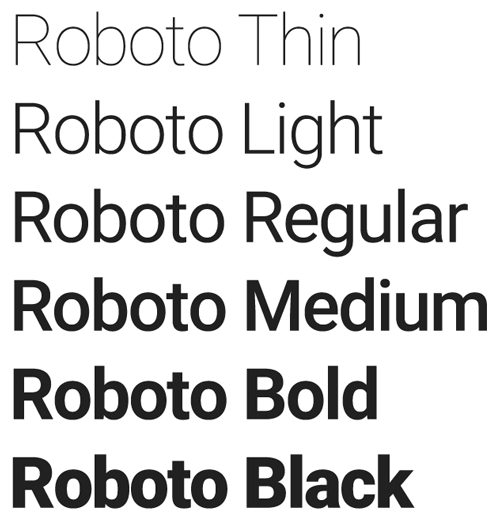
\includegraphics[scale=0.2]{doc/imagenes/roboto.png}}
    \caption{Fuente ''Roboto'' de Google Material}
    \label{roboto}
\end{figure}

Además, se seguirán los siguientes tamaños de fuente proporcionados por la guía de diseño de Google Material para los distintos formatos de texto (Figura \ref{font-size}):

\begin{figure}[H]
    \centering{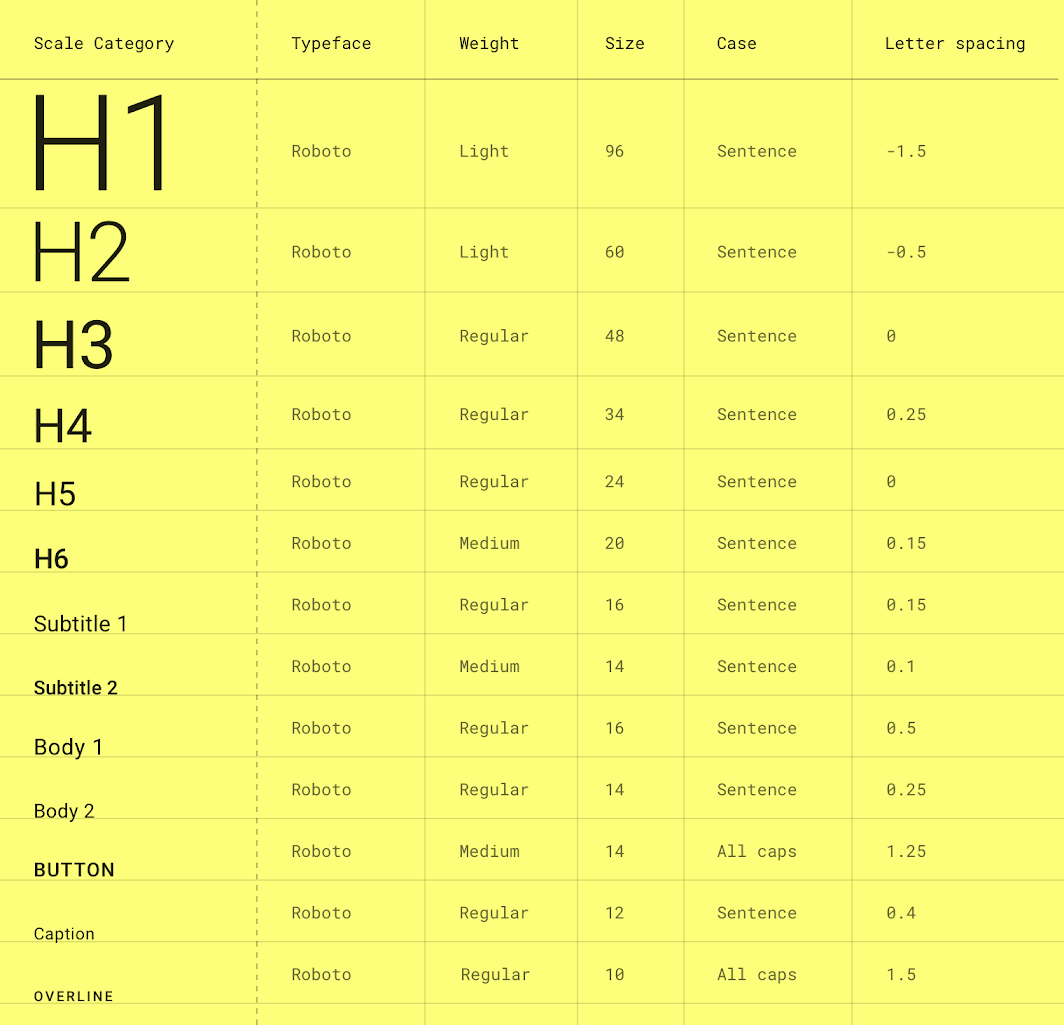
\includegraphics[scale=0.2]{doc/imagenes/font-size.png}}
    \caption{Tamaños de fuente para ''Roboto'' según las guías de diseño de Google Material}
    \label{font-size}
\end{figure}

Finalmente, a continuación se muestra el logo de DayDay (Figura \ref{logo-dayday}), el cual ha sido diseñado en el editor online Figma:

\begin{figure}[H]
    \centering{
\includegraphics[scale=0.1]{doc/imagenes/DayDay_logo.png}}
    \caption{Logo de DayDay}
    \label{logo-dayday}
\end{figure}

Como cuadro resumen de lo explicado, se recoge todo lo expuesto anteriormente en el siguiente Moodboard (Figura \ref{moodboard}):

\begin{figure}[H]
    \centering{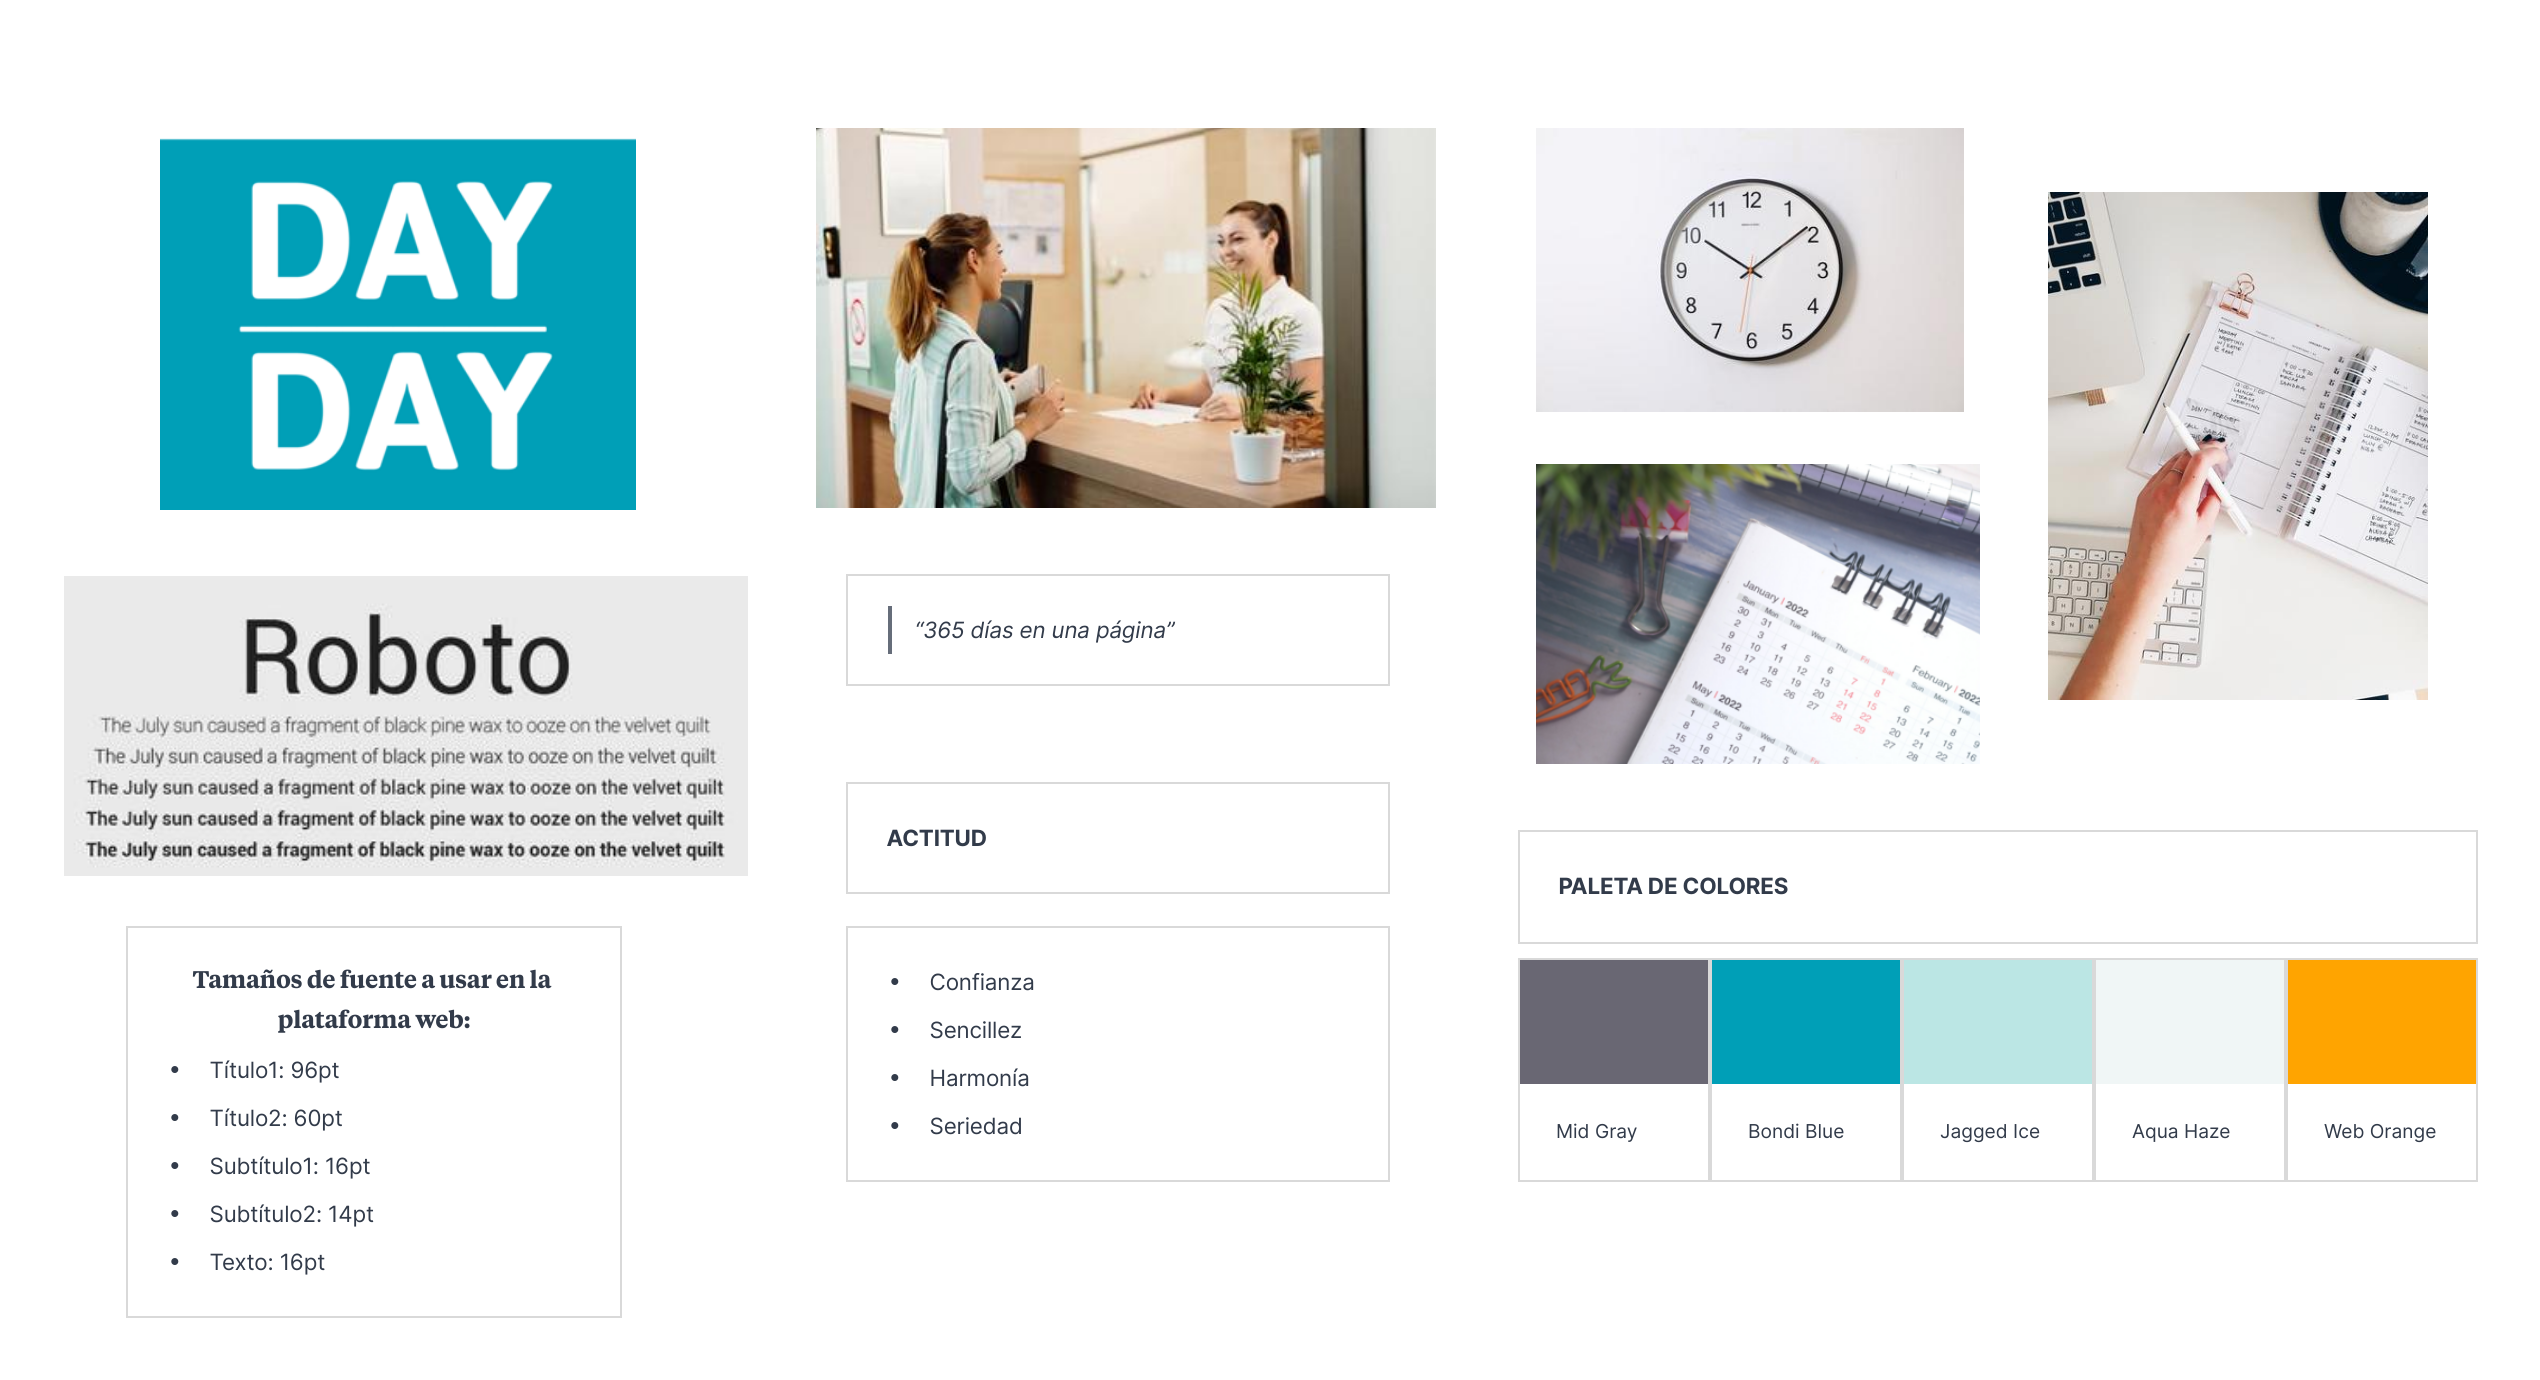
\includegraphics[scale=0.15]{doc/imagenes/moodboard.png}}
    \caption{Moodboard de DayDay}
    \label{moodboard}
\end{figure}

\subsubsection{Wireframes y Mockups} \label{mockup-wirefram}
Tras implantar las guías de diseño que seguirá DayDay es momento de crear los diseños de la interfaz, para ello utilizamos la herramienta Figma.

Primeramente se han preparado unos wireframes que servirán para establecer el entramado de la interfaz de DayDay (Figuras \ref{wireframe-login}, \ref{wireframe-calendario}, \ref{wireframe-pacientes}, \ref{wireframe-psicologos}, \ref{wireframe-perfil}, \ref{wireframe-crear-cita}, \ref{wireframe-editar-cita} y \ref{wireframe-cambiar-contraseña} ):

\begin{figure}[H]
    \centering{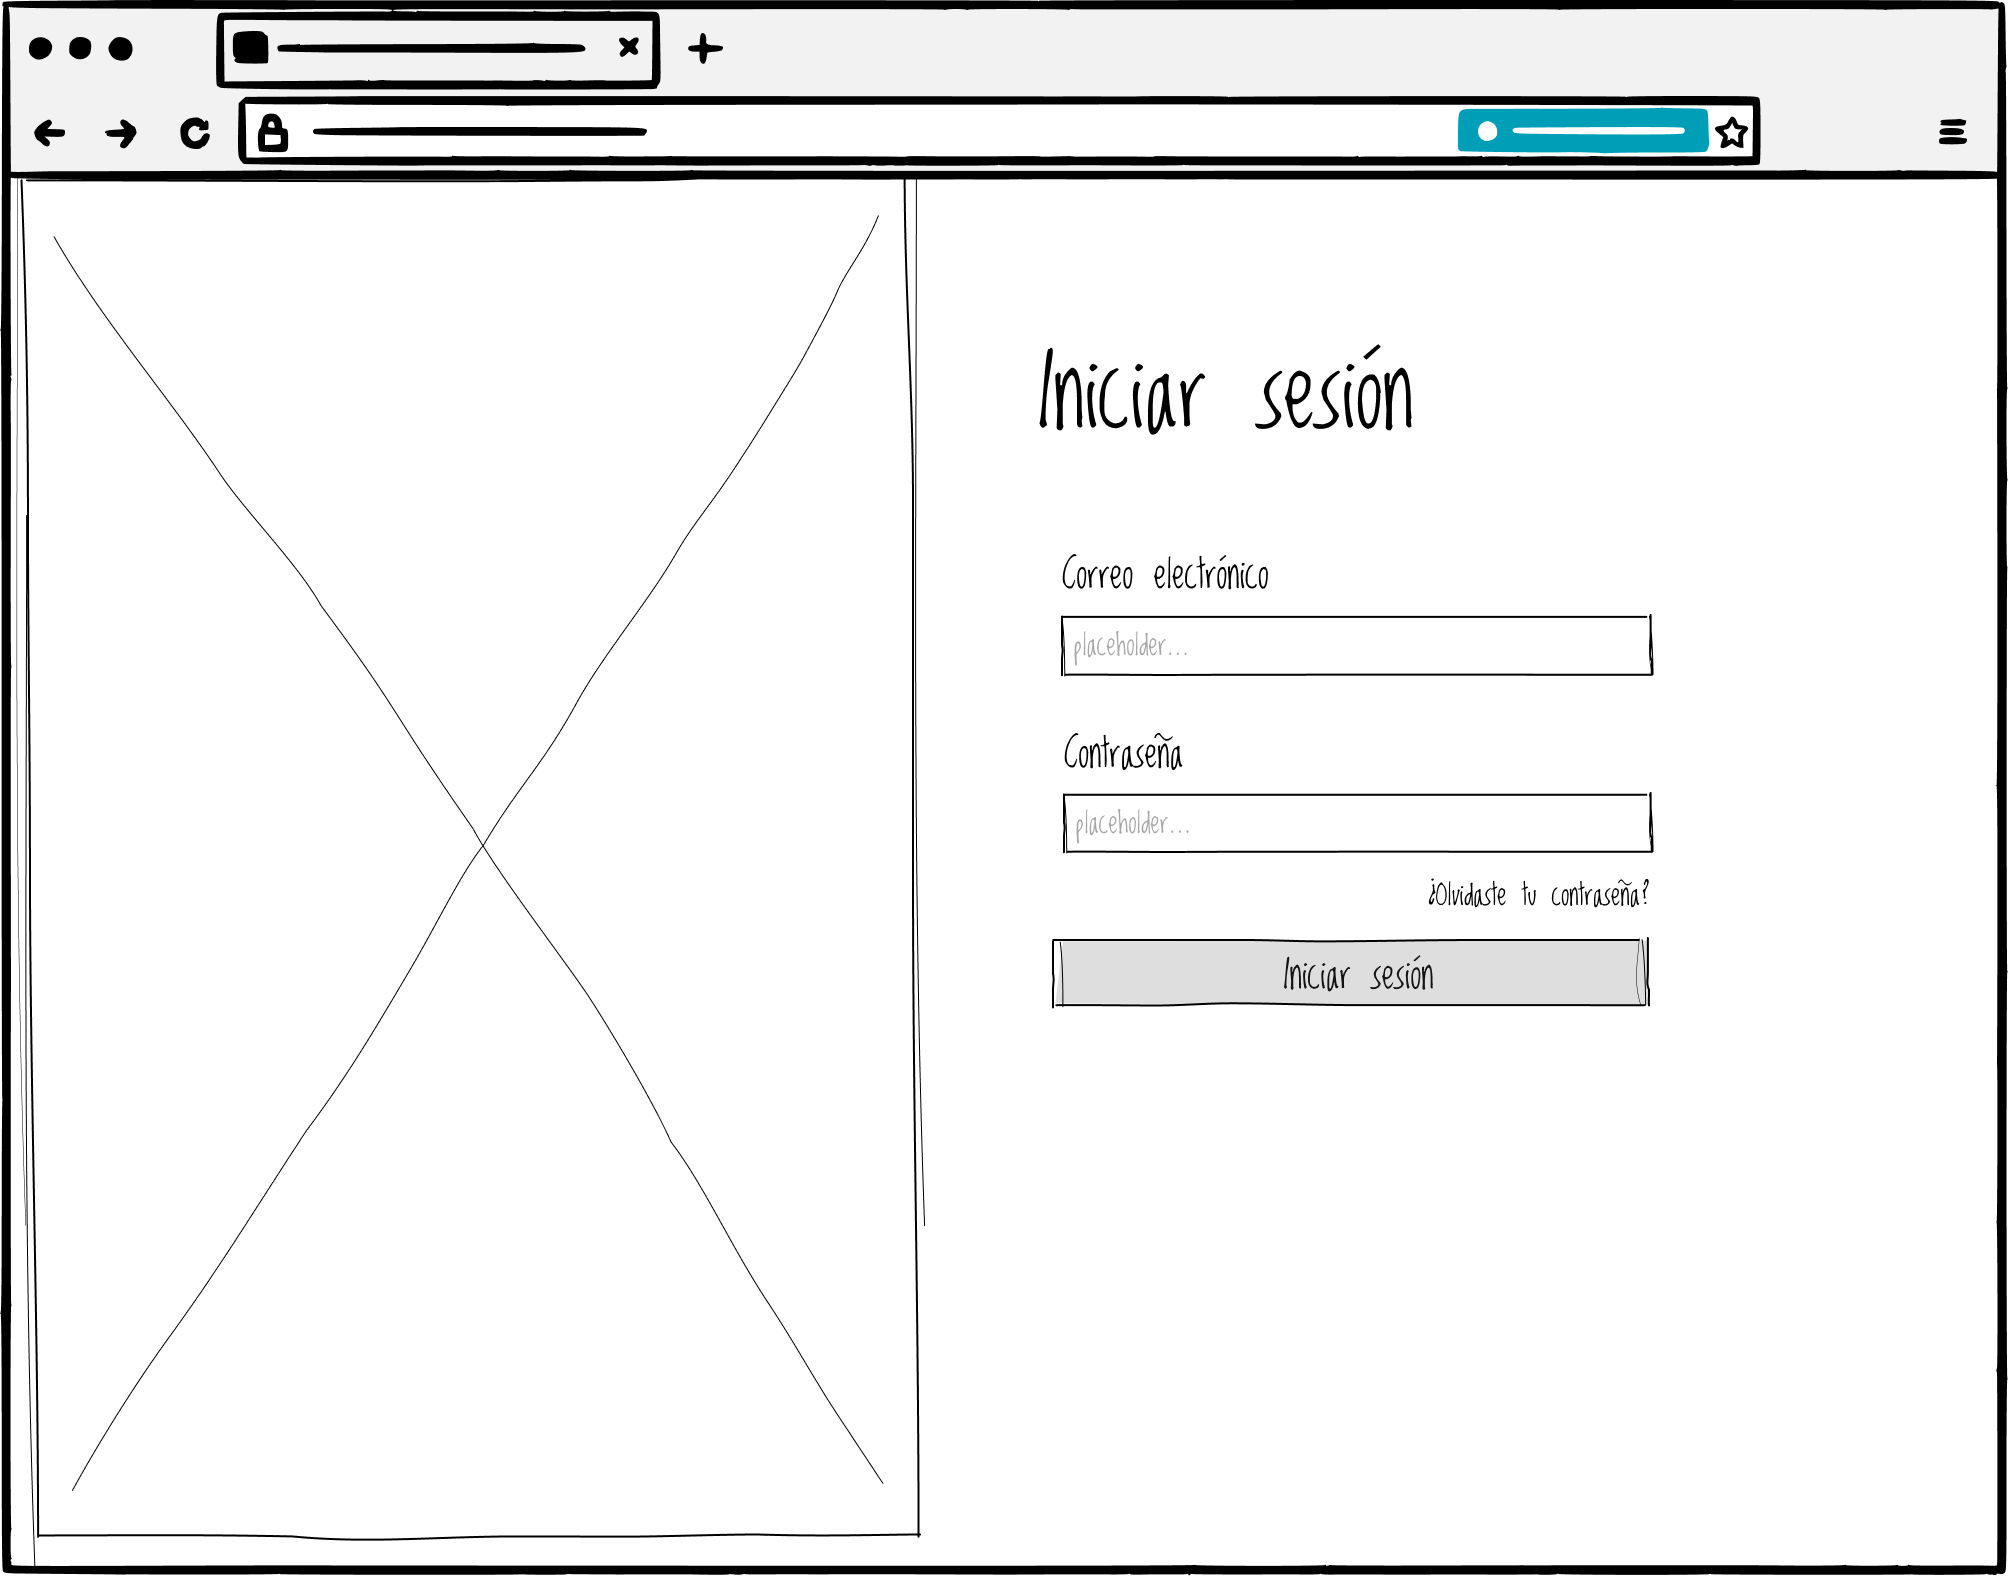
\includegraphics[scale=0.1]{doc/imagenes/vista-login.png}}
    \caption{Wireframe de la vista de Iniciar sesión}
    \label{wireframe-login}
\end{figure}

\begin{figure}[H]
    \centering{\includegraphics[scale=0.1]{doc/imagenes/vista-calendario.png}}
    \caption{Wireframe de la vista de Calendario}
    \label{wireframe-calendario}
\end{figure}

\begin{figure}[H]
    \centering{\includegraphics[scale=0.1]{doc/imagenes/vista-pacientes.png}}
    \caption{Wireframe de la vista de Pacientes}
    \label{wireframe-pacientes}
\end{figure}

\begin{figure}[H]
    \centering{\includegraphics[scale=0.1]{doc/imagenes/vista-psicologos.png}}
    \caption{Wireframe de la vista de Psicólogos}
    \label{wireframe-psicologos}
\end{figure}

\begin{figure}[H]
    \centering{\includegraphics[scale=0.1]{doc/imagenes/vista-perfil.png}}
    \caption{Wireframe del diálogo de Perfil}
    \label{wireframe-perfil}
\end{figure}

\begin{figure}[H]
    \centering{\includegraphics[scale=0.1]{doc/imagenes/dialogo-crear-cita.png}}
    \caption{Wireframe del diálogo de crear cita}
    \label{wireframe-crear-cita}
\end{figure}

\begin{figure}[H]
    \centering{\includegraphics[scale=0.1]{doc/imagenes/dialogo-editar-cita.png}}
    \caption{Wireframe del diálogo de editar cita}
    \label{wireframe-editar-cita}
\end{figure}

Teniendo estos wireframes como guías para el diseño final de la plataforma, seguidamente se diseñaron los mockups en los que en algunos se hicieron algunas modificaciones en la estructura planteada en una primera instancia por los wireframes (Figuras \ref{mockup-login}, \ref{mockup-calendario}, \ref{mockup-menu} \ref{mockup-pacientes}, \ref{mockup-psicologos}, \ref{mockup-perfil}, \ref{mockup-add} y \ref{mockup-edit}). Sobretodo cabe mencionar que el menú lateral ha pasado a ser un desplegable. 

\begin{figure}[H]
    \centering{\includegraphics[scale=0.2]{doc/imagenes/mockup-login.png}}
    \caption{Mockup de la vista de Login}
    \label{mockup-login}
\end{figure}

\begin{figure}[H]
    \centering{\includegraphics[scale=0.2]{doc/imagenes/mockup-calendario (1).png}}
    \caption{Mockup de la vista de Calendario}
    \label{mockup-calendario}
\end{figure}

\begin{figure}[H]
    \centering{\includegraphics[scale=0.2]{doc/imagenes/mockup-menu.png}}
    \caption{Mockup de la vista de Calendario con el menú desplegado}
    \label{mockup-menu}
\end{figure}

\begin{figure}[H]
    \centering{\includegraphics[scale=0.2]{doc/imagenes/mockup-pacientes.png}}
    \caption{Mockup de la vista de Pacientes}
    \label{mockup-pacientes}
\end{figure}

\begin{figure}[H]
    \centering{\includegraphics[scale=0.2]{doc/imagenes/mockup-psicologos.png}}
    \caption{Mockup de la vista de Psicólogos}
    \label{mockup-psicologos}
\end{figure}

\begin{figure}[H]
    \centering{\includegraphics[scale=0.2]{doc/imagenes/mockup-perfil.png}}
    \caption{Mockup de la vista de Perfil}
    \label{mockup-perfil}
\end{figure}

\begin{figure}[H]
    \centering{\includegraphics[scale=0.2]{doc/imagenes/mockup-add.png}}
    \caption{Mockup de la vista del diálogo de crear cita}
    \label{mockup-add}
\end{figure}

\begin{figure}[H]
    \centering{\includegraphics[scale=0.2]{doc/imagenes/mockup-edit.png}}
    \caption{Mockup de la vista del diálogo de editar cita}
    \label{mockup-edit}
\end{figure}


    % Implementación y pruebas
    \chapter{Implementación y pruebas}
Siguiendo con lo definido en el Capítulo \ref{disenio}, donde se han definido los tres bloques que forman el stack MEAN, en este capítulo se procederá a la explicación de su implementación. Para ello, de igual forma al capítulo anterior, se ha hecho una separación de los tres bloques en los que primeramente se expondrá la especificación de las herramientas necesarias para el desarrollo procurando escoger las versiones LTS para seguir durante un número determinado de años recibiendo actualizaciones de soporte. Por supuesto, se describirá el proceso llevado a cabo de programación y, como toda buena implementación, ésta será acompañada de las pruebas que correspondan para corroborar el correcto funcionamiento de la plataforma.

\section{Implementación del servidor y de la base de datos} \label{implementacion-server}
En este apartado se expondrán las herramientas y el procedimiento llevado a cabo para el desarrollo del servidor y el establecimiento de la base de datos utilizada por este. Es destacable mencionar, que previamente se ha hecho una investigación y aprendido Node.js y Express a través de distintos tutoriales y con el libro \textit{''Web development with node and express: leveraging the JavaScript stack''} para tomar las bases de ambas tecnologías \cite{brown2019web}

\subsection{Herramientas para el desarrollo}
Por un lado, para la base de datos se ha utilizado \textbf{MongoDB} haciendo uso del servicio proporcionado en la nube de \textbf{MongoDB Atlas} para la administración de bases de datos MongoDB. En dicho servicio se ha elegido el clúster gratuito con ubicación en París por cercanía, de 512Mb el cual utiliza la versión de MongoDB 5.0.6. 

Por otro lado, para el servidor se han escogido las versiones LTS de \textbf{Node.js} y \textbf{Express} las cuales son 18.12 y 4.18, respectivamente. Por supuesto la utilización de dichas herramientas implica una implementación con el lenguage de programación \textbf{JavaScript}. Además, es muy importante destacar la utilización del administrador de procesos \textbf{PM2} version 5.2 que permite tener dos instancias totalmente iguales del servidor, una activa y otra \textit{''dormida''}, de forma que si la activa falla se despierta a la segunda instancia y se crea una nueva dormida. Por último, para probar las llamadas a la API se ha elegido \textbf{Postman}.

\subsection{Proceso de desarrollo}
Para dar comienzo a la implementación de DayDay se ha creado primeramente la base de datos con nombre ''dd\_db'' junto con las collecciones ya descritas en la Sección \ref{bd}. \bigskip

Con la base de datos ya creada, es momento de crear el servidor y conectarlo a esta. Dadas las colecciones definidas de \textbf{usuarios} y \textbf{citas} se ha hecho una separación de ambas entidades en los \textbf{controladores} de Node.js encargados de toda la lógica de la plataforma, así como los \textbf{modelos} que definen la estructura de los documentos de dichas colecciones. A continuación se precisa la lógica que lleva cada controlador:

\begin{itemize}
    \item \textbf{Controlador de usuarios}: Encargado de toda la lógica CRUD referente a los usuarios. En este controlador se ha de destacar la creación de usuarios, pues los usuarios son creados sin contraseña. Para el establecimiento de ella se le manda al usuario un email de activación de cuenta con un enlace que contiene como parámetro un token JWT previamente generado a partir de una clave secreta almacenada en el fichero \textit{.env} que redirige al usuario al cliente para que pueda establecer su contraseña. Para poder llevar a cabo la emisión de este email se utiliza un módulo de Node.js llamado \textbf{nodemailer} que utiliza como ''host'' Gmail y las credenciales de un correo electrónico creado para la plataforma. Exactamente de igual forma, se procede en la función encargada de enviar el correo para la recuperación de contraseña. Por supuesto, en cada función de este controlador se hace una comprobación previa del rol del usuario para darle o no permiso a realizar la operación, en caso de que éste no lo tuviera se mandaría un código de error 401.
    \item \textbf{Controlador de citas}: Este controlador es el corazón de la plataforma DayDay, en este caso encargado de todas las operaciones CRUD referentes a las citas y en particular hay dos funciones que resultan clave y las cuales hay que resaltar. Para crear una cita asociada a un psicólogo se debe de conocer previamente su disponibilidad, para ello se ha creado una primera función responsable de devolver el rango de horas disponibles para el comienzo de una cita de cinco en cinco minutos. Para lo cual la función recibe el día en el que se quiere realizar la cita y partiendo desde la hora de apertura hasta la hora de cierre de la clínica y habiendo obtenido las citas previamente reservadas se establece que una hora estará disponible teniendo en cuenta que las citas tienen un mínimo de duración de una hora si: 
    \begin{itemize}
        \item No coincide con la hora inicio de otra cita ya reservada.
        \item Desde dicha hora hasta pasada una hora exacta no existe dentro de ese intervalo otra cita.
        \item La hora de después de esa hora no es posterior al cierre de la clínica.
    \end{itemize}  
    Una vez es conocida la hora de inicio deseada para un día y un psicólogo en concreto, la segunda función nos permite conocer los horas disponibles de fin de una cita, pues las citas pueden ser tan extensas como quiera el paciente siempre y cuando no interfiera con la cita de otro. Siguiendo esto, las horas de fin disponibles de una cita serán aquellas que comiencen una hora después de la hora de inicio elegida y estas son incrementadas de cinco en cinco minutos y consideradas disponibles hasta interferir con la hora de inicio de otra cita.
\end{itemize}

Para poder acceder a las funcionalidades dadas por estos controladores y construir un servidor con Node.js se ha utilizado Express, herramienta la cual ha permitido registrar las distintas rutas de la API a las que podrá acceder el cliente (Figura \ref{fig:rutas}): 

\begin{figure}[H]
    \centering{\includegraphics[scale=0.4]{doc/imagenes/rutas.png
    }}
    \caption{Rutas de la API de DayDay}
    \label{fig:rutas}
\end{figure}

De la Figura \ref{fig:rutas} hay que resaltar las funciones \textbf{''login''}, \textbf{''authenticateToken''} y \textbf{''checkToken''}. Estas tres funciones pertenecen a un tercer controlador responsable de la autenticación y autorización en la plataforma. En primer lugar la función ''login'' es la utilizada para el inicio de sesión en la plataforma en la que se chequea si las credenciales son correctas y si lo son se procede a la generación de un token JWT firmado con una clave secreta cuyo ''payload'' es el email del usuario. Una vez generado el JWT se manda como cookie en la respuesta que contiene el email, id, nombre, apellidos y rol del usuario en formato JSON. Resulta muy importante destacar que para tener la mayor seguridad posible en la API siguiendo lo establecido en el artículo \textit{''A Case Study on Cookies and Cyber Security''} \cite{kumawatcase}, las cookies se han establecido como \textbf{''httpOnly''} para que la cookie sólo sea accesible a través de HTTP, \textbf{''sameSite''} para sólo poder enviar la cookie al contexto propio y por último \textbf{''secure''} para que sólo se manden exclusivamente por HTTPS. Para proteger el resto de rutas a las que no puede acceder un usuario que no se haya indentificado en la plataforma se utiliza la función ''authenticateToken'' a modo de middleware para verficar que la cookie enviada en la petición es válida, si lo es se continuará con la petición, en caso contrario se retornará un 401. En cuanto a la función ''checkToken'', esta es llamada en aquellas peticiones en las que se quiera comprobar un token desde el cliente, lo cual se llevará acabo para el acceso a las vistas de activación de cuenta o reestablecimiento de contraseña. \bigskip

En referente a lo que concierne a la gestión y conexión con la base de datos se ha utilizado el módulo \textbf{mongoose} que ha permitido hacer una especificación de los esquemas de las colecciones de citas y usuarios y la conexión con la base de datos encontrada en MongoDB Atlas utilizando la URI proporcionada.

Por último, debido a que el proceso de un servidor Node.js Express deja de funcionar si ocurre un fallo en la API se ha decidido utilizar PM2 para hacer una gestión de ello. Para lo cual, como se ha descrito con anterioridad, se ha creado un archivo \textbf{''.process.js''} que contiene la siguiente configuración para lanzar 2 instancias (Figura \ref{fig:pm2}):

\begin{figure}[H]
    \centering{\includegraphics[scale=0.4]{doc/imagenes/pm2.png
    }}
    \caption{Configuración de PM2}
    \label{fig:pm2}
\end{figure}


\section{Implementación del cliente}
Al igual que en el apartado anterior (Sección \ref{implementacion-server}), a continuación se indicarán las herramientas utilizadas en la implementación del cliente así como el proceso llevado a cabo para su programación. 

\subsection{Herramientas para el desarrollo}
Para el desarrollo del cliente de la plataforma se ha utilizado Node.js con su versión LTS 18.12 utilizado para la gestión de módulos y \textbf{Angular} con la versión 14.2 que es la más reciente, aunque no LTS debido a problemas de incompatibilidad con la versión de Node.js. Dentro del framework de Angular utilizaremos las herramientas clásicas en el desarrollo web: 
 \begin{itemize}
     \item \textbf{HTML} para la estructuración de la web.
     \item \textbf{SCSS} el cual es un lenguage de hojas de estilo que utiliza la sintaxis de CSS y hereda las propiedades del metalenguaje de hojas de estilo SaaS permitiendo así la posibilidad ofrecida de declaración de variables en hojas de estilo. 
     \item \textbf{TypeScript} lenguage de programación utilizado en Angular para crear las funciones utilizadas por los componentes web.
 \end{itemize}

Además, se utilizarán las siguientes librerías:
\begin{itemize}
    \item \textbf{Angular Material}, librería de componentes de Angular desarrollada por Google.
    \item \textbf{Angular Flex} para conseguir una interfaz responsiva.
    \item \textbf{RxJS}, librería que sigue el patrón \textbf{Observador} que es un diseño de patrón software en el que a un objeto se le suscriben varios para recibir eventos si su estado cambiase. Esto será de gran utilidad para evitar refrescos cuando algún componente de la vista cambie su estado.
\end{itemize}

En cuanto al componente protagonista, el calendario, se planteó utilizar un componente de Angular ya desarrollado para ahorrar tiempo. Tras hacer una investigación se encontraron algunas opciones, pero la mayoría fueron descartadas ya que eran de pago o por su poco atractiva interfaz. Es por esto que finalmente entre todas ellas destacó el componente Angular Schedule de Syncfusion \footnote{\url{https://ej2.syncfusion.com/angular/documentation/schedule/}}.

\subsection{Proceso de desarrollo}
Ahora que conocemos las herramientas usadas para el desarrollo del cliente, hemos diseñado los mockups en la Sección \ref{mockup-wirefram} y creado la API finalmente es momento de añadir la pieza final a DayDay, el cliente. \bigskip

Para la comunicación con la API, Angular dispone de unas funciones conocidas como \textbf{''servicios''}. Se han creado cuatro, siendo los tres primeros encargados de llamar a las rutas expuestas en la Figura \ref{fig:rutas}:

\begin{itemize}
    \item \textbf{Servicio de citas}
    \item \textbf{Servicio de usuarios}
    \item \textbf{Servicio de autenticación y autorización}
    \item \textbf{Servicio de snackbar}, es un servicio el cual hace uso de un componente de Angular Material que precisa de un servicio para poder funcionar. Es encargado de mostrar una notificación por pantalla cuando fuera requerido
\end{itemize}

En cuanto a los componentes que conforman la vista se distinguen los siguientes:

\begin{itemize}
    \item \textbf{Componentes accesibles por usuarios no identificaciones}:
    \begin{itemize}
        \item \textbf{Login}, vista dedicada al inicio de sesión en la plataforma utilizado el servicio de autenticación y de autorización
        \item \textbf{Recuperación de contraseña}, muestra un formulario para mandar un email de reestablecimiento de contraseña a la dirección de correo electrónico introducida. Para ello hace uso del servicio de usuarios.
        \item \textbf{Página 404}: Si no existe ninguna ruta asociada a la ruta especificada en el navegador es el componente al que el usuario será redirigido por defecto.
    \end{itemize}
    \item \textbf{Componentes accesibles por todos los roles (administrador, psicólogo y paciente)}:
    \begin{itemize}
        \item \textbf{Calendario}: Es el componente más complejo de la plataforma, en él se ha hecho uso del componente \textbf{''Angular Schedule'' de Syncfusion}. Para este proyecto la interfaz del componente ha tenido que ser bastante moldeada para ajustarse a los requisitos impuestos. Para ello, se han alterados las propiedades CSS de las clases definidas en su HTML en los ficheros SCSS y además se han reemplazado los valores de algunas variables del propio componente a través de HTML como se muestra en la Figura \ref{fig:html-calendar}
        \begin{figure}[H]
            \centering{\includegraphics[scale=0.4]{doc/imagenes/html-calendar.png
            }}
            \caption{HTML del componente Schedule de Syncfusion con propiedades modificadas}
            \label{fig:html-calendar}
        \end{figure}
        Para mostrar las citas este componente recibe como fuente de datos un array de JSONs que sigue la estructura del definida en la colección de citas \ref{bd}. En cuanto a la realización de operaciones CRUD con ellas se llama a las funciones \textbf{''onPopupOpen()''} y \textbf{''onPopupClose()''} que reciben como parámetro la información de la celda del calendario a la que se le ha hecho click (hora de inicio de la celda, hora de fin de la celda, fecha y si contiene una cita, toda la información referente a esa cita). Dentro de dichas funciones se lleva a cabo la gestión del formulario que contiene el diálogo emergente para la creación, edición y eliminación de una cita. Dentro de ese diálogo, gracias a RxJS, si el psicólogo seleccionado o la hora de inicio seleccionada cambiaran, las horas disponibles de inicio y fin se verían actualizadas sin refrescar la página. De igual forma es así una vez que se ha creado, añadido o eliminado una cita en el calendario de Syncfusion.
        Este componente hace uso del servicio de citas.
        \item \textbf{Perfil}: Diálogo emergente que muestra la información del usuario actual que se encuentra almacenada en el almacenamiento local del navegador. Además, a través de este componente el usuario puede cambiar su contraseña haciendo uso del servicio de usuarios.
        \item \textbf{Menú lateral}: El menú lateral es visible para todos los roles, sin embargo las opciones mostradas en él son variantes en función de si el rol del usuario tiene permiso o no para acceder a ellas.
    \end{itemize}
    \item \textbf{Componentes accesibles por el administrador}
    \begin{itemize}
        \item \textbf{Lista de pacientes} y \textbf{lista de psicólogos}: Permite la gestión completa de los pacientes y psicólogos. En ambos componentes se abren diálogos emergentes que contienen ''subcomponentes'':
        \begin{itemize}
            \item \textbf{Formulario de creación de pacientes} y \textbf{formulario de creación de psicólogos}
            \item \textbf{Formulario de edición de pacientes} y \textbf{formulario de edición de psicólogos}
            \item \textbf{Formulario de eliminación de pacientes} y \textbf{formulario de eliminación de psicólogos}
        \end{itemize}
        Todos los componentes listados con anterioridad recurren al servicio de usuarios. 
        
        En cuanto a las listas, debido a que se está utilizando el componente \textit{'''mat-table'''} de Angular Material que no permite la actualización de datos sin refresco, la página es recargada cuando se lleva a cabo una operación sobre un paciente. 
    \end{itemize}
    \item \textbf{Componente accesibles con un token válido}
    \begin{itemize}
        \item \textbf{Activación de cuenta}: Vista para que el usuario estableczca una contraseña para su cuenta en la plataforma. Utiliza el servicio de usuarios
        \item \textbf{Reestablecimiento de contraseña}: Vista que permite al usuario establecer una nueva contraseña para su cuenta
    \end{itemize}
\end{itemize}

\subsubsection*{Seguridad}
Tratándose de una plataforma para un centro sanitario, la seguridad en el cliente es crucial. Por ello, se han llevado a cabo una serie de medidas acompañadas a las medidas de seguridad del servidor. \bigskip

Debido a que el servidor es el encargado de hacer las comprobaciones de que el usuario es quien dice ser a través de las cookies, si el cliente recibiera un código 401 la aplicación siempre redireccionará al usuario a la vista de login y tendrá que volver a iniciar sesión para acceder a ella. ¿Cómo se logra esto? A través de los \textbf{interceptores HTTP} de Angular (Figura \ref{fig:interceptor}) responsable de analizar todas las respuestas recibidas al cliente.

\begin{figure}[H]
    \centering{\includegraphics[scale=0.35]{doc/imagenes/interceptor.png
    }}
    \caption{Interceptor HTTP de Angular}
    \label{fig:interceptor}
\end{figure}

En cuanto al acceso restringido a la vistas, se ha creado un \textbf{''Guard''} de Angular (Figura \ref{fig:guard}) el cual obtiene los roles permitidos para la vista a la que se va a navegar y si el rol del usuario identificado no se encuentra entre ellos se le redireccionará a la página 404

\begin{figure}[H]
    \centering{\includegraphics[scale=0.35]{doc/imagenes/guard.png
    }}
    \caption{Role Guard de Angular}
    \label{fig:guard}
\end{figure}

Finalmente, las vistas de activación de cuenta y reestablecimiento de contraseña en las que el usuario sólo posee un token, son sólo accesibles si la función ''\textbf{checkToken()}'' del servidor envía un código 200.

\section{Pruebas}
Son numerosas las posibilidades a elegir para realizar pruebas en Node.js como Jest, Jasmine, AVA o Mocha que son los más populares. Todos ellos son de código abierto, no existen apenas diferencias entre ellos y tras hacer una investigación en la documentación oficial de Node.js en este no se indica en ningún momento qué herramienta es la más conveniente utilizar. Por ello, se han analizado las herramientas nombras en cuanto a uso en la página web ''npm trends'' \footnote{\url{https://npmtrends.com/ava-vs-jasmine-vs-jest-vs-mocha}} y se ha observado (Figura \ref{fig:tests-stats}) que las dos primeras posiciones las ocupan Jest y Mocha:

\begin{figure}[H]
    \centering{\includegraphics[scale=0.25]{doc/imagenes/test-stats.png
    }}
    \caption{Número de descargas en el último año de Jest, Jasmine, AVA y Mocha}
    \label{fig:tests-stats}
\end{figure}

Tomando esto en cosideración y haciendo un pequeño estudio sobre ambas herramientas, finalmente se decidió utilizar \textbf{Mocha} junto con la librería \textbf{Chai}. La principal razón para tomar esta decisión fue lo que bien afirma Santiago Toscanini et al. en su trabajo titulado ''Fundamentos de entrega continua y tecnologías para pipelines de
desarrollo de software'' \cite{toscanini2022fundamentos}, y es que Mocha es más flexible y configurable que Jest. Aunque Jest es más sencillo en cuanto a configuraciones, éste se encuentra más orientado a las pruebas en frontend. \bigskip

En la realización de pruebas para el backend se han planteado tests para cada uno de los endpoints de la Figura \ref{fig:rutas}:

\begin{itemize}
    \item \textbf{Métodos de los endpoints de autorización y autenticación}:
    \begin{itemize}
        \item \textbf{login()}: Se hace una petición enviando un email y contraseña correctos y se espera un código de estado 200 y la existencia de una cookie en la respuesta.
        \item \textbf{checkToken()}: Con una cookie previamente obtenida se envía el JWT de esta haciendo la petición correspondiente y se espera como respuesta un código 200.
    \end{itemize}
    \item \textbf{Métodos de los endpoints de usuarios} (Para realizar la prueba de todas estos métodos previamente se ha debido de haber iniciado sesión a través del endpoint de ''/api/login''):
    \begin{itemize}
        \item \textbf{addUser(), getPatients() y getPsychologists()}: Se envía una petición con todos los datos de un usuario psicólogo, se espera un código 201 y se listan todos los usuarios con ''getPsychologists()'' se obtiene el último creado y se comprueba que el id del usuario creado y el obtenido coinciden. De igual forma se ha probado la adición de un usuario paciente con el endpoint de ''getPatients()'' pasándole como psicólogo asignado el id del psicólogo creado anteriormente.
        \item \textbf{editPatient() y editPsychologist()}: Se edita el nombre del paciente/psicólogo creado anteriormente, se vuelven a listar los pacientes/psicólogos y se obtiene el editado. Si el nombre editado y el introducido coinciden el test es válido.
        \item \textbf{getPatientPsychologist()}: Con el id del paciente creado anteriormente, se pide al endpoint su psicólogo y si el id que retorna coincide con el id del psicólogo creado anteriormente el test es válido.
        \item \textbf{forgetPassword()}: Se envía una petición con el correo electrónico de uno de los usuarios creados anteriormente y se espera un código 201.
        \item \textbf{setPassword()}: Se envía una petición con el correo electrónico de uno de los usuarios creados anteriormente y se espera un código 201.
        \item \textbf{deleteUser()}: Con los ids obtenidos de los anteriores usuarios creado se llama al endpoint y si se recibe un código 201 el test ha sido pasado con éxito.
    \end{itemize}
    \item \textbf{Métodos de los endpoints de citas}:
    \begin{itemize}
        \item \textbf{getAvailableStartAppointments()}: Para un psicólogo previamente creado se piden las horas disponibles para éste un día en concreto. Si la primera hora disponible son las 10:00 el test es correcto
        \item \textbf{getAvailableEndAppointments()}: Para un psicólogo previamente creado y una hora de inicio de cita seleccionada, si la primera hora disponible es una hora después de la seleccionada el test es correcto
        \item \textbf{addAppointment(), editAppointment(), getAppointments(), deleteAppointment()}: se crea una nueva cita para un psicólogo y paciente previamente creados y para una fecha de inicio y fin de cita seleccionadas. Se espera un código de estado 201 como respuesta, si este test es pasado con éxito se listan las citas y el id de la cita listada tiene que coincidir con la creada. Finalmente se edita la hora de fin de una cita y se vuelve a listar ésta, si coincide la introducida con la cita listada el test ha sido pasado con éxito y la cita es borrada esperándose un código de estado 201.
    \end{itemize}
    
\end{itemize}






    % Despliegue
    \chapter{Despliegue} \label{despliegue}

Con la plataforma ya funcionando en la máquina local es momento de proceder a su despliegue. Actualmente existen múltiples posibilidades para realizar el despliegue de una aplicación web como DigitalOcean, OpenShift, AWS o Microsoft Azure. Tras una comparación de precios se ha elegido \textbf{AWS}, en concreto el servicio \textbf{EC2} que es una máquina virtual que representa un servidor físico, por su barato coste, fiabilidad, seguridad, fácil uso y rapidez para llevar a cabo el despliegue. Para facilitar el despliegue se ha decidido ''dockerizar'' la plataforma con \textbf{Docker} y \textbf{Docker Compose}. Además, se ha utilizado \textbf{Cloudfare} para realizar la compra de un dominio y de \textbf{Let's Encrypt} para la generación gratuita de un certificado SSL diseñado para acelerar la adopción de HTTPS, como bien se indica en el artículo \textit{''Let’s Encrypt: An Automated Certificate
Authority to Encrypt the Entire Web''} \cite{aas2019let}. \bigskip

Así pues, una vez se conocen qué herramientas van a ser utilizadas para llevar a cabo el despliegue, seguidamente se explicará el proceso seguido para ello habiendo investigado previamente cómo llevarlo a cabo a través del libro de Shimon Ifrah \cite{ifrah2019installing}.

\section{Proceso del despliegue}
Primeramente, como se ha comentado en la introducción al capítulo, se ha ''dockerizado'' la plataforma. Para ello se han creado tres archivos: dos \textbf{dockerfiles} para el cliente y para el servidor y un \textbf{docker-compose.yaml} para la orquestación de los dos contenedores docker. Veamos a continuación cada uno por separado:

\begin{itemize}
    \item \textbf{Dockerfile del servidor} (Figura \ref{fig:docker-back}): Se ha elegido la imagen de ''node:18-12-alpine'' ya que la versión 18.12 es la versión LTS de Node.js. Tras especificar dicha versión, se ha establecido el directorio de trabajo en el mostrado en la (Figura \ref{fig:docker-back}) y se ha llevado a cabo la instalación de las dependencias del servidor junto con PM2 para finalmente exponer el contenedor docker en el puerto 8080 y lanzar el servidor.
    
    \begin{figure}[H]
        \centering{\includegraphics[scale=0.35]{doc/imagenes/docker-back.png
        }}
        \caption{Dockerfile del servidor}
        \label{fig:docker-back}
    \end{figure}
    
    \item \textbf{Dockerfile del cliente} (Figura \ref{fig:docker-front}): El dockerfile del cliente se ha planteado de igual forma al del servidor, con una pequeña diferencia. Se trata de la instalación de las dependencias instaladas en la aplicación de Angular que se encuentran alojadas en el fichero ''package.json''. En cuanto al puerto, se ha elegido el 4200 ya que la aplicaciones de Angular típicamente son expuestas en este puerto.
    
    \begin{figure}[H]
        \centering{\includegraphics[scale=0.35]{doc/imagenes/docker-front.png}}
        \caption{Dockerfile del cliente}
        \label{fig:docker-front}
    \end{figure}

    \item\textbf{Fichero Docker Compose} (Figura \ref{fig:docker-compose}): Para el fichero '''docker-compose.yaml''' se han establecido dos servicios, uno para el cliente y otro para el servidor. Se han mantenido ambos puertos para la máquina local, pero cuando se haga el despliegue el puerto del cliente, que es el que quedará abierto para acceder a la página, será cambiado de 4200 a 443 que es el puerto usado por HTTPS.

    \begin{figure}[H]
        \centering{\includegraphics[scale=0.35]{doc/imagenes/docker-compose.png}}
        \caption{Fichero Docker Compose}
        \label{fig:docker-compose}
    \end{figure}
\end{itemize}


Ahora que el proyecto ha sido dockerizado y con una cuenta ya creada en AWS, se lanza la instancia EC2. Esta tarea resulta algo compleja, ya que implica hacer un pequeño estudio del consumo de memoria y CPU de los contenedores docker para su configuración. Gracias a la orden '''docker stats''' podemos visualizar dichas métricas (Figura \ref{fig:docker-stats}):

    \begin{figure}[H]
        \centering{\includegraphics[scale=0.35]{doc/imagenes/docker-stats.png}}
        \caption{Consumo de los contenedores docker del servidor y del cliente}
        \label{fig:docker-stats}
    \end{figure}

Teniendo estas métricas presentes, la configuración escogida para la instancia ha sido la siguiente:
\begin{itemize}
    \item \textbf{Sistema operativo}: Debido a que
    a que pertenece al plan gratuito, se ha escogido la imagen del sistema operativo Linux de Amazon con la arquitectura presentada en la Figura \ref{fig:ec2-imagen}:
    \begin{figure}[H]
        \centering{\includegraphics[scale=0.25]{doc/imagenes/imagen-aws.png}}
        \caption{Imagen escogida para la instancia de EC2}
        \label{fig:ec2-imagen}
    \end{figure}
    \item \textbf{Tipo de instancia}: Son numerosas los tipos de instancias ofrecidas para EC2, pero visualizando la Figura \ref{fig:docker-stats} donde se aprecia un consumo de ran de casi 1GiB por parte del contenedor del cliente y entorno a 80MiB por parte del servidor, se ha barajado entre escoger una instancia ''t2.small'' o ''t3.medium'' (Figura \ref{fig:ec2-types}). Finalmente, se ha optado por la segunda opción con el objetivo de evitar limitaciones de RAM:
    \begin{figure}[H]
        \centering{\includegraphics[scale=0.25]{doc/imagenes/aws-type.png}}
        \caption{Tipos de instancias EC2 junto con sus características y precios}
        \label{fig:ec2-types}
    \end{figure}
    \item \textbf{Grupos de seguridad}: Finalmente se han establecido los grupos de seguridad, que funcionan a modo de firewall dictando quin puede entrar a la instancia. En este caso se han establecido tres: SSH, HTTP y HTTPS, a través de los cuales todo el mundo pueda acceder a la plataforma (Figura \ref{fig:ec2-security}):
    \begin{figure}[H]
        \centering{\includegraphics[scale=0.25]{doc/imagenes/aws-security.png}}
        \caption{Grupos de seguridad establecidos para la instancia EC2}
        \label{fig:ec2-security}
    \end{figure}
\end{itemize}

Con esta configuración lista ya se puede lanzar la instancia y hacer la conexión vía ssh a ella. Una vez se ha realizado la conexión se procede a descargar el repositorio de Github de este proyecto y se lanza la orden '''docker-compose up'''.  \bigskip

Por último, se ha hecho la compra del dominio ''dayday-calendar.win'' en Cloudfare. Se ha escogido este dominio en específico debido a ser el que más bajo coste tenía y se le han asignado la IPs pública de la instancia EC2 (Figura \ref{fig:dns})

    \begin{figure}[H]
        \centering{\includegraphics[scale=0.25]{doc/imagenes/dns.png}}
        \caption{Asignación de la IP pública de la instancia EC2 al dominio}
        \label{fig:dns}
    \end{figure}

Para acabar, creamos una zona alojada con el servicio ''Route 53'' de AWS para el dominio de Cloudfare. Esto es necesario para gestionar la dirección del tráfico hacia un dominio en específico (Figura \ref{fig:aws-zone}):

    \begin{figure}[H]
        \centering{\includegraphics[scale=0.25]{doc/imagenes/aws-zone.png}}
        \caption{Zonas alojadas para la instancia}
        \label{fig:aws-zone}
    \end{figure}

En cuanto a la generación del certificado se ha hecho uso de las indicaciones dadas por la página oficial de Let's Encrypt donde indican que a través de la ejecución del cliente \textbf{Certbot} ,que deberá previamente ser instalado en la instancia, y se crearán el archivo del certificado y la llave de éste. 

    % Conclusiones y trabajos futuros
    \chapter{Conclusiones y trabajos futuros}



    \newpage
    \chapter*{Glosario}

\begin{itemize}
    \item \textbf{Historia de usuario}: En un marco de trabajo ágil, se define historia de usuario como una descripción simple de una funcionalidad dicha por un usuario que la desea. 
    \item \textbf{EC2}: En AWS EC2 es una instancia de un servidor virtual para correr aplicaciones en la infraestructura de AWS.
    \item \textbf{Route 53}: Servicio para manejar el DNS para otros servicios y máquinas desplegadas en AWS.
    \item \textbf{Stack software}: Es una colección independiente de componentes que trabajan juntos en la ejecución de una aplicación.
    \item \textbf{Sitemap}: Es una mapa en el que se estructura y organizan las distintas páginas que conforman un sitio web
    \item \textbf{Moodboard}: Es un tablero en el que se recogen ideas de forma visual a modo de ''collage'' formado de imágenes, texto, colores.
    \item \textbf{Wireframes}: Diagrama de baja fidelidad que rerpresenta el esqueleto de un sitio web
    \item \textbf{LTS}: Se trata del ''Soporte a Largo Plazo'' que son versiones de un software diseñadas para ser matenidas en un largo periodo de tiempo.
    \item \textbf{Zona alojada}: En AWS se trata de un contenedor de registros en el cual los registros indican cómo el tráfico es redireccionado a un dominio en específico.
\end{itemize}
    
	\newpage
	\bibliography{bibliografia}
	\bibliographystyle{plain}
	
\end{document}

